% A LaTeX template for MSc Thesis submissions to 
% Politecnico di Milano (PoliMi) - School of Industrial and Information Engineering
%
% S. Bonetti, A. Gruttadauria, G. Mescolini, A. Zingaro
% e-mail: template-tesi-ingind@polimi.it
%
% Last Revision: October 2021
%
% Copyright 2021 Politecnico di Milano, Italy. NC-BY

\documentclass{Configuration_Files/PoliMi3i_thesis}
%------------------------------------------------------------------------------
%	REQUIRED PACKAGES AND  CONFIGURATIONS
%------------------------------------------------------------------------------

% CONFIGURATIONS
\usepackage{rotating, caption}
\usepackage{pdflscape}
\usepackage{pdfpages}
\usepackage{minted}
\usepackage{comment}
\usepackage{listings}
\usepackage{parskip} % For paragraph layout
\usepackage{setspace} % For using single or double spacing
\usepackage{emptypage} % To insert empty pages
\usepackage{multicol} % To write in multiple columns (executive summary)
\setlength\columnsep{15pt} % Column separation in executive summary
\setlength\parindent{0pt} % Indentation
\raggedbottom  
\usepackage{silence}


% PACKAGES FOR TITLES
\usepackage{titlesec}
% \titlespacing{\section}{left spacing}{before spacing}{after spacing}
\titlespacing{\section}{0pt}{3.3ex}{2ex}
\titlespacing{\subsection}{0pt}{3.3ex}{1.65ex}
\titlespacing{\subsubsection}{0pt}{3.3ex}{1ex}
\usepackage{color}

% PACKAGES FOR LANGUAGE AND FONT
\usepackage[english]{babel} % The document is in English  
\usepackage[utf8x]{inputenc} % UTF8 encoding
\usepackage[T1]{fontenc} % Font encoding
\usepackage[11pt]{moresize} % Big fonts

% PACKAGES FOR IMAGES
\usepackage{graphicx}
\usepackage{transparent} % Enables transparent images
\usepackage{eso-pic} % For the background picture on the title page
\usepackage{subfig} % Numbered and caption subfigures using \subfloat.
\usepackage{tikz} % A package for high-quality hand-made figures.
\usetikzlibrary{}
\graphicspath{{./Images/}} % Directory of the images
\usepackage{caption} % Coloured captions
\usepackage{xcolor} % Coloured captions
\usepackage{amsthm,thmtools,xcolor} % Coloured "Theorem"
\usepackage{float}
\usepackage{wrapfig}

% STANDARD MATH PACKAGES
\usepackage{amsmath}
\usepackage{amsthm}
\usepackage{amssymb}
\usepackage{amsfonts}
\usepackage{bm}
\usepackage[overload]{empheq} % For braced-style systems of equations.
\usepackage{fix-cm} % To override original LaTeX restrictions on sizes

% PACKAGES FOR TABLES
\usepackage{tabularx}
\usepackage{longtable} % Tables that can span several pages
\usepackage{colortbl}
\usepackage{multirow}
\usepackage{longtable}
% PACKAGES FOR ALGORITHMS (PSEUDO-CODE)
\usepackage{algorithm}
\usepackage{algorithmic}
\usepackage{blindtext}


\usepackage[absolute]{textpos}
\usepackage{fancyhdr}
\fancypagestyle{lscape}{% 
\fancyhf{} % clear all header and footer fields 
\fancyfoot[LE]{%
\begin{textblock}{20}(1,5){\rotatebox{90}{\leftmark}}\end{textblock}
\begin{textblock}{1}(13,10.5){\rotatebox{90}{\thepage}}\end{textblock}}
\fancyfoot[LO] {%
\begin{textblock}{1}(13,10.5){\rotatebox{90}{\thepage}}\end{textblock}
\begin{textblock}{20}(1,13.25){\rotatebox{90}{\rightmark}}\end{textblock}}
\renewcommand{\headrulewidth}{0pt} 
\renewcommand{\footrulewidth}{0pt}}


% PACKAGES FOR REFERENCES & BIBLIOGRAPHY
%\usepackage[colorlinks=true,linkcolor=black,anchorcolor=black,citecolor=black,filecolor=black,menucolor=black,runcolor=black,urlcolor=black]{hyperref} % Adds clickable links at references
%\usepackage{cleveref}
%\usepackage[square, numbers, sort&compress]{natbib} % Square brackets, citing references with numbers, citations sorted by appearance in the text and compressed
%\bibliographystyle{siam} % You may use a different style adapted to your field

% PACKAGES FOR REFERENCES & BIBLIOGRAPHY
\usepackage[colorlinks=true,linkcolor=black,anchorcolor=black,citecolor=black,filecolor=black,menucolor=black,runcolor=black,urlcolor=black]{hyperref} % Adds clickable links at references
\usepackage{cleveref}
\usepackage[square, numbers, sort&compress]{natbib} % Square brackets, citing references with numbers, citations sorted by appearance in the text and compressed
\bibliographystyle{abbrvnat} % You may use a different style adapted to your field


% OTHER PACKAGES
\usepackage{pdfpages} % To include a pdf file
\usepackage{afterpage}
\usepackage{lipsum} % DUMMY PACKAGE
\usepackage{fancyhdr} % For the headers
\usepackage{xcolor}
\fancyhf{}
\usepackage{eurosym}

% Input of configuration file. Do not change config.tex file unless you really know what you are doing. 
% Define blue color typical of polimi
\definecolor{bluepoli}{cmyk}{0.4,0.1,0,0.4}

% Custom theorem environments
\declaretheoremstyle[
  headfont=\color{bluepoli}\normalfont\bfseries,
  bodyfont=\color{black}\normalfont\itshape,
]{colored}

% Set-up caption colors
\captionsetup[figure]{labelfont={color=bluepoli}} % Set colour of the captions
\captionsetup[table]{labelfont={color=bluepoli}} % Set colour of the captions
%\captionsetup[algorithm]{labelfont={color=bluepoli}} % Set colour of the captions

\theoremstyle{colored}
\newtheorem{theorem}{Theorem}[chapter]
\newtheorem{proposition}{Proposition}[chapter]

% Enhances the features of the standard "table" and "tabular" environments.
\newcommand\T{\rule{0pt}{2.6ex}}
\newcommand\B{\rule[-1.2ex]{0pt}{0pt}}

% Pseudo-code algorithm descriptions.
%\newcounter{algsubstate}
%\renewcommand{\thealgsubstate}{\alph{algsubstate}}
%\newenvironment{algsubstates}
 % {\setcounter{algsubstate}{0}%
  % \renewcommand{\STATE}{%
   %  \stepcounter{algsubstate}%
    % \Statex {\small\thealgsubstate:}\space}}
  %{}

% New font size
\newcommand\numfontsize{\@setfontsize\Huge{200}{60}}

% Title format: chapter
\titleformat{\chapter}[hang]{
\fontsize{50}{20}\selectfont\bfseries\filright}{\textcolor{bluepoli} \thechapter\hsp\hspace{2mm}\textcolor{bluepoli}{|   }\hsp}{0pt}{\huge\bfseries \textcolor{bluepoli}
}

% Title format: section
\titleformat{\section}
{\color{bluepoli}\normalfont\Large\bfseries}
{\color{bluepoli}\thesection.}{1em}{}

% Title format: subsection
\titleformat{\subsection}
{\color{bluepoli}\normalfont\large\bfseries}
{\color{bluepoli}\thesubsection.}{1em}{}

% Title format: subsubsection
\titleformat{\subsubsection}
{\color{bluepoli}\normalfont\large\bfseries}
{\color{bluepoli}\thesubsubsection.}{1em}{}

% Shortening for setting no horizontal-spacing
\newcommand{\hsp}{\hspace{0pt}}

\makeatletter
% Renewcommand: cleardoublepage including the background pic
\renewcommand*\cleardoublepage{%
  \clearpage\if@twoside\ifodd\c@page\else
  \null
  \AddToShipoutPicture*{\BackgroundPic}
  \thispagestyle{empty}%
  \newpage
  \if@twocolumn\hbox{}\newpage\fi\fi\fi}
\makeatother

%For correctly numbering algorithms
%\numberwithin{algorithm}{chapter}

%----------------------------------------------------------------------------
%	NEW COMMANDS DEFINED
%----------------------------------------------------------------------------

% EXAMPLES OF NEW COMMANDS
\newcommand{\bea}{\begin{eqnarray}} % Shortcut for equation arrays
\newcommand{\eea}{\end{eqnarray}}
\newcommand{\e}[1]{\times 10^{#1}}  % Powers of 10 notation

%----------------------------------------------------------------------------
%	ADD YOUR PACKAGES (be careful of package interaction)
%----------------------------------------------------------------------------
%\usepackage{pgfplots}
\usepackage{lscape}
\usepackage{rotating}
\usepackage{lipsum}


%----------------------------------------------------------------------------
%	ADD YOUR DEFINITIONS AND COMMANDS (be careful of existing commands)
%----------------------------------------------------------------------------
\newsavebox{\mybox}
%----------------------------------------------------------------------------
%	BEGIN OF YOUR DOCUMENT
%----------------------------------------------------------------------------




\begin{document}


\fancypagestyle{plain}{%
\fancyhf{} % Clear all header and footer fields
\fancyhead[RO,RE]{\thepage} %RO=right odd, RE=right even
\renewcommand{\headrulewidth}{0pt}
\renewcommand{\footrulewidth}{0pt}}

%----------------------------------------------------------------------------
%	TITLE PAGE
%----------------------------------------------------------------------------

\pagestyle{empty} % No page numbers
\frontmatter % Use roman page numbering style (i, ii, iii, iv...) for the preamble pages

\puttitle{
	title=Controlling management systems applied to LPT Italian companies, % Title of the thesis
	name= \\ 
	      \vspace{0.2 cm}\\
	      Chiara Beretta \hspace{2,2 cm} 10615536 \\ 
          \vspace{0.01 cm}  \\   
          Seyed Hesam Babaei \hspace{0,98 cm} 10780315 \\ 
          \vspace{0.01 cm}\\ 
          Luca Cattaneo \hspace{2,3 cm} 10521219 \\ 
          \vspace{0.01 cm}\\          
          Pietro Mariano \hspace{2,2 cm} 10502703 \\
          \vspace{0.01 cm}\\
          Fabio Vitiello \hspace{2,6 cm} 10529938, % Author Name and Surname
	course= MOBILITY: INFRASTRUCTURES AND SERVICES , % Study Programme (in Italian)
	academicyear={2021/2022},  % Academic Year
} % These info will be put into your Title page 

%----------------------------------------------------------------------------
%	PREAMBLE PAGES: ABSTRACT (inglese e italiano), EXECUTIVE SUMMARY
%----------------------------------------------------------------------------
\startpreamble
\setcounter{page}{1} % Set page counter to 1

% ABSTRACT IN ENGLISH

%\include{Chapters/00_Abstract}

%----------------------------------------------------------------------------
%	LIST OF CONTENTS/FIGURES/TABLES/SYMBOLS
%----------------------------------------------------------------------------

% TABLE OF CONTENTS
\thispagestyle{empty}
\tableofcontents % Table of contents 
\thispagestyle{empty}
\cleardoublepage

%-------------------------------------------------------------------------
%	THESIS MAIN TEXT
%-------------------------------------------------------------------------
% In the main text of your thesis you can write the chapters in two different ways:
%
%(1) As presented in this template you can write:
%    \chapter{Title of the chapter}
%    *body of the chapter*
%
%(2) You can write your chapter in a separated .tex file and then include it in the main file with the following command:
%    \chapter{Title of the chapter}
%    \input{chapter_file.tex}
%
% Especially for long thesis, we recommend you the second option.

%\addtocontents{toc}{\vspace{2em}} % Add a gap in the Contents, for aesthetics
\mainmatter % Begin numeric (1,2,3...) page numbering
% --------------------------------------------------------------------------
% NUMBERED CHAPTERS % Regular chapters following
% --------------------------------------------------------------------------
\chapter{Introduction}
The purpose of this project is to design a dashboard with financial and economical KPIs, in order to provide trends and values to verify and monitor the company's performances. We have 

We expanded the work, adding a new objective, as shown in the figure \ref{fig:concmap} below, representing the general outline of our project.


\begin{figure}[h]
    \centering
    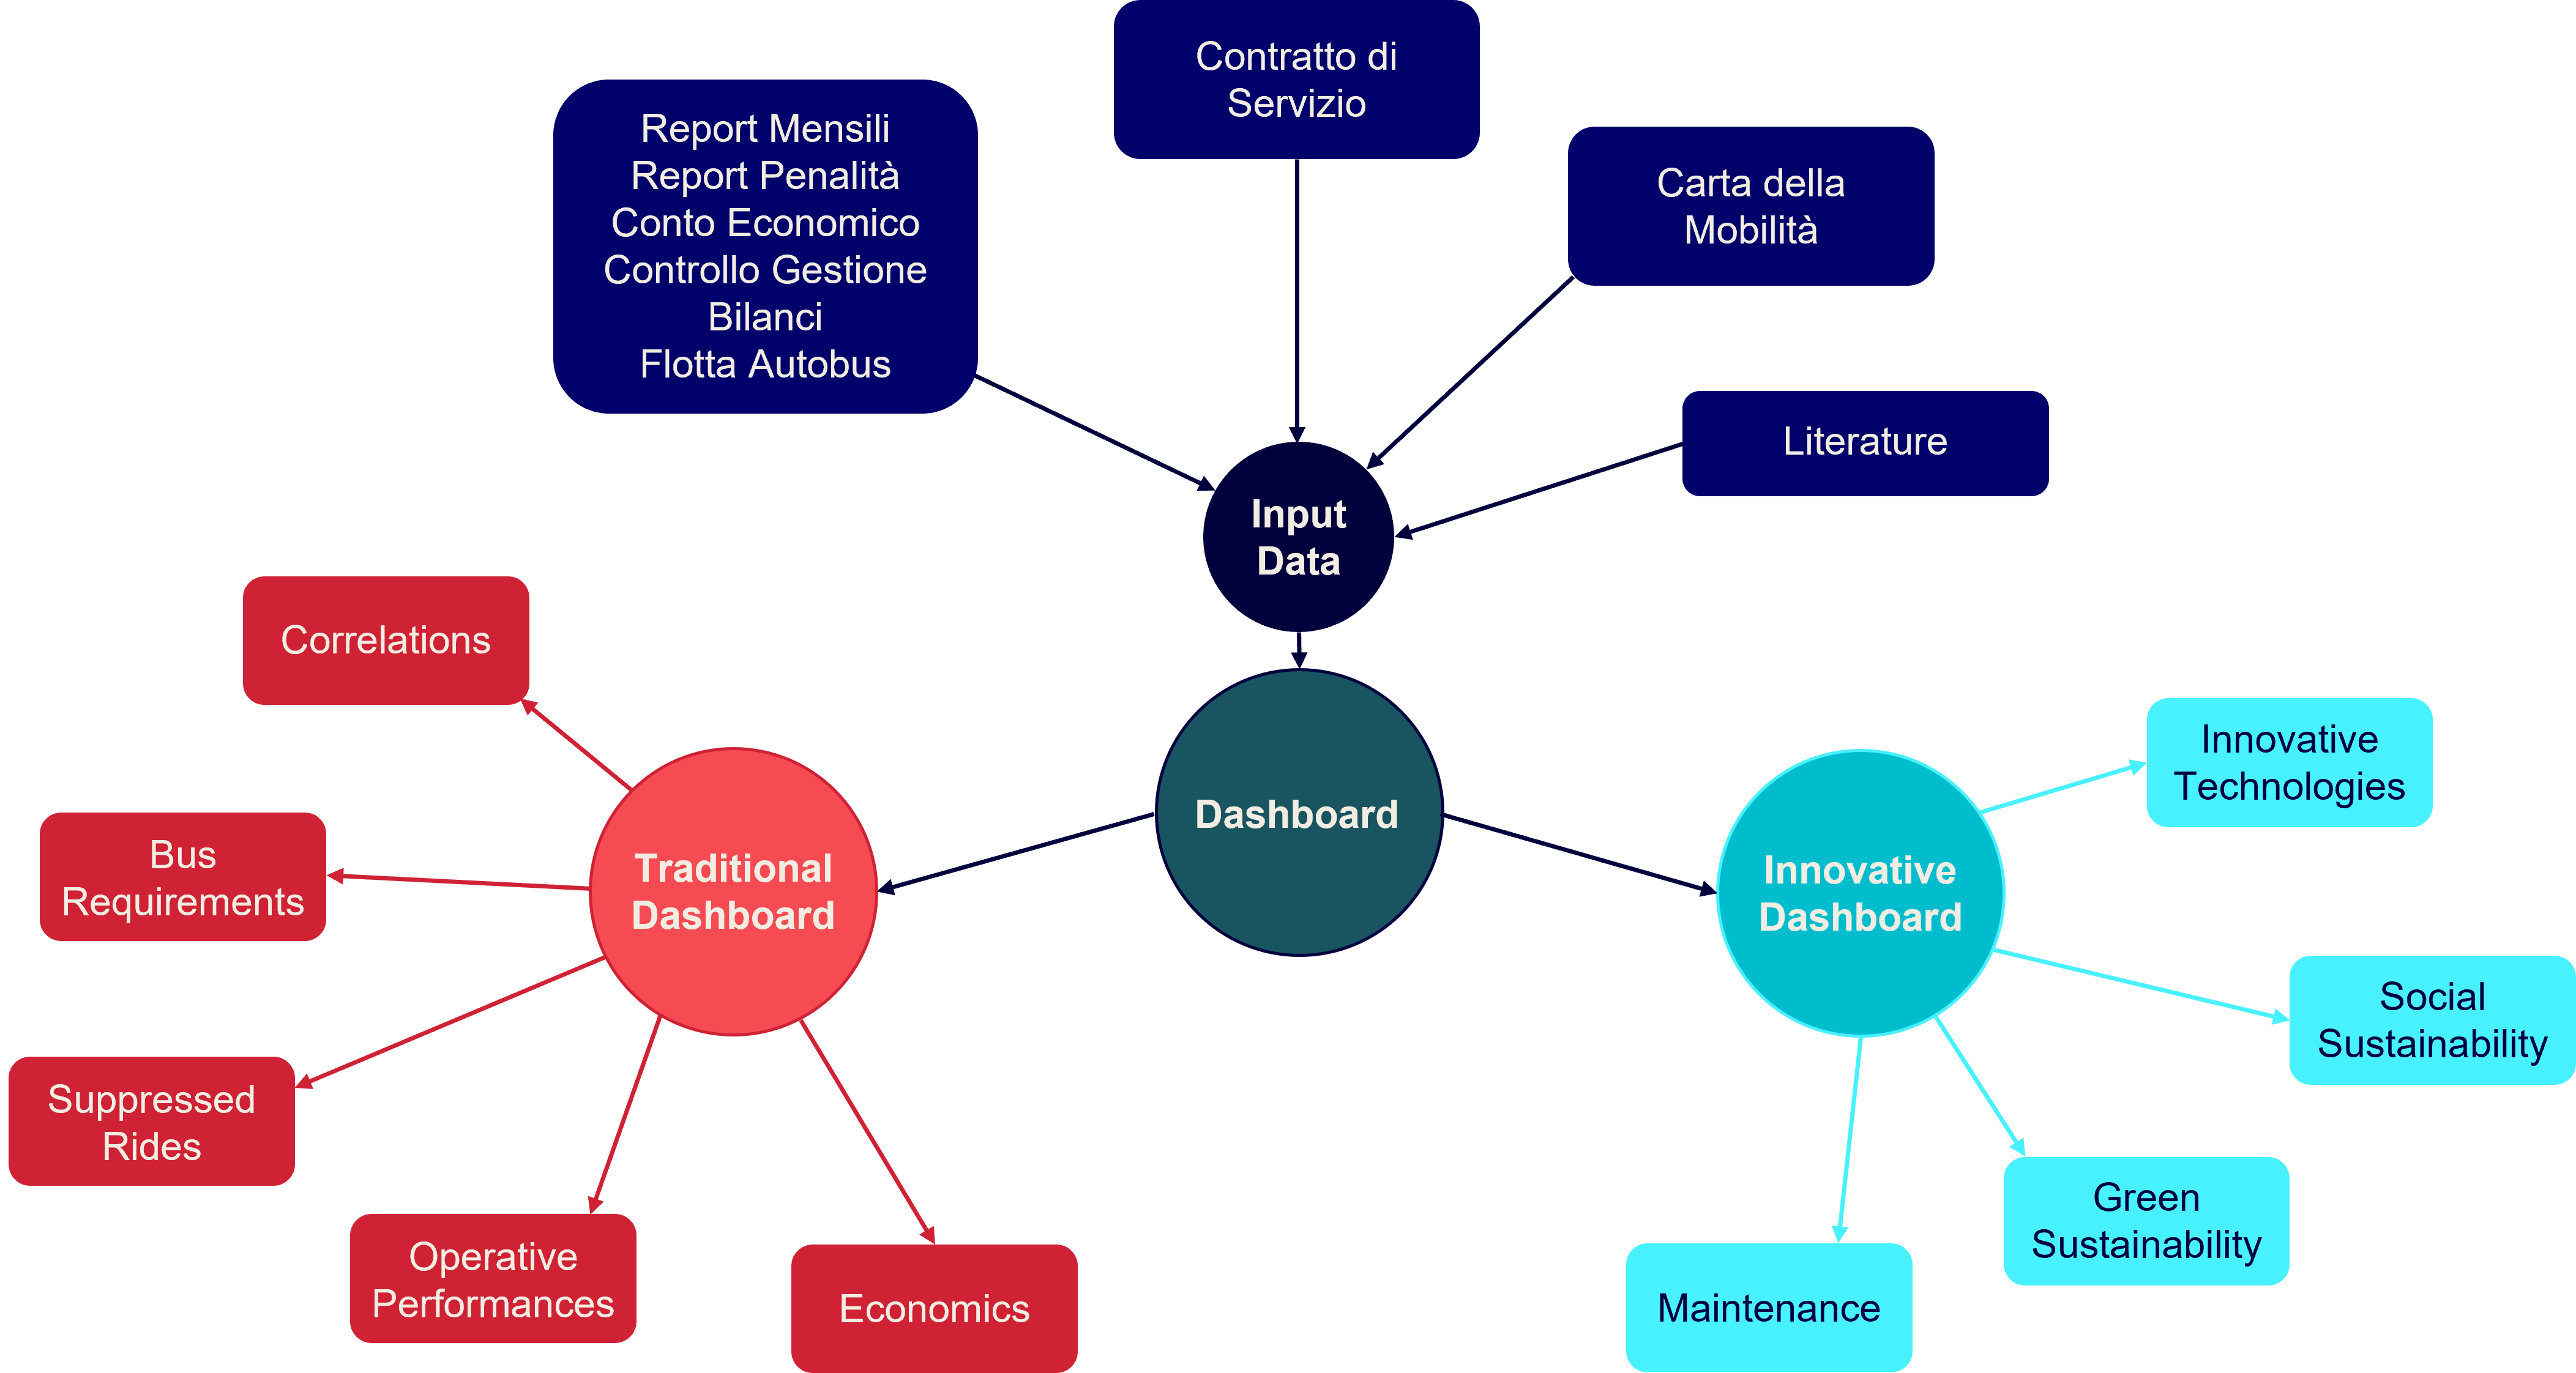
\includegraphics[width=1\textwidth]{Images/intro_scheme.png}
    \caption{Conceptual Map of the work}
    \label{fig:concmap}
\end{figure}

First of all, a presentation of the study case has been made with an analysis of the service
contract and a short history recap of the public service in the Subnetwork SUD of the
Province of Bergamo (that starts in 2004). From this, we have been found some KPIs useful
to monitor and check the compliance with the requirements of the service contract (for
example: bus fleet requirements, suppressed rides, ...).

Using the datasets provided by Arriva we first have done a data cleaning, in order to create a dashbpard that could work on three main levels: consortium's companies, lines and time (month or year). Along with the dashboard a work of investigation and comment of the result have been presented with the aim of discuss and highlight the potential of the work.

Taking in consideration also the current changes in the world and in particular in the mobility sector (COVID-19 before and now the energy crisis due to Ukraine war) and  the objectives of ONU \cite{sdgs}, the second part talk about how to implement new aspects of this sector in a new and innovative dashboard; we will assess analyses on new technologies of public transport, different perspectives on sustainability such as green and social, concluding with a focus on maintenance procedures of new buses.

%FINITO
\date{\today}

















\chapter{State of the Art}

\paragraph{What is Arriva}
Arriva Italia is the Arriva Group’s italian branch. Present on the Italian market since 2002, managing around $5\%$ of the market shares, it provides both urban and extra-urban transport services mainly in Northern Italy, as well as shuttle services to Turin and Milan airports.

With respect to our case study Arriva Italia is member of the Bergamo Trasporti consortium from the 2002 with the acquisition of \emph{SAB Autoservizi} and directly from 2020 with the incorporation of SAB.

\subparagraph{The Consortium}
The Consortium is an association of different companies built in 2003 for the tender about the Subnetwork SUD of the Province of Bergamo.
The different companies that are part of the consortium are: \emph{SAI Società Autolinee Interprovinciali srl, Arriva Italia srl, AGI Auto Guidovie Italiane SpA, Autoservizi Locatelli srl, TBSO Trasporti Bergamo Sud Ovest SpA e Autoservizi Zani srl.}

\paragraph{What is a dashboard}
As reported on the official website of Microsoft a dashboard is a tool to track, analyze and display data about a process or an organization to obtain insight.

The benefits are different such as performance measure, data transparency and forecasting.


\subparagraph{Apllication on the LPT\cite{rossiPTM}}

In our study case the dashboard can be a useful instrument to allow both the PTO and PTA check the respect of the requirements provided from the contract of service. Then the PTO can define useful relation between the KPIs themselves. 

So, to start our analysis the Service contract must be read and analyzed.
\section{Analysis of Contract of Service}
\label{sec:contract}
%Analysis of the contract of service. From that  the defined KPI  to put in "traditional dashboard"
\paragraph{What is a service contract?}
%explain what is the service contract and some background in the context
The service contract regulates the discharge of a public service by an operator as decided by the public authority. In case of public transport the authority is called PTA and the operator PTO. The service contract are generally made after a tender and are regulated by the REGULATION (EC) No. 1370/2007 at European level and by the Italian legislative decree No. 422/2007 that respectively define the norms about the public transport service on road and rails and assign the function to the different Italian local entities.

\paragraph{The case of study: Bergamo Trasporti Consortium}
The case of study is about the public transport service of the subnetwork sud (the so called "pianura Bergamasca") of the province of Bergamo (with the Province of Bergamo as PTA) and the Bergamo trasporti consortium as PTO.

\subparagraph{History of the service} The service started in 2005 after the winning of the tender by the consortium in 2004. Then a first extension was made in 2011 (the natural expiration year) until 2014 without changes in the requirements. Then another extension was made with changes in the contract of service in particular:
\begin{itemize}
    \item Required number of $bus-km\cdot year$ risen up to $4.345.000$
    \item Grants
    \item Bus fleet
\end{itemize}

Then in 2019, the PTA used the power provided by the article 5 of REGULATION (EC) No 1370/2007 and use the \emph{requirement to provide} to extend the duration of the contract of service until 31/12/2021. This act also changed the previous requirements/conditions:
\begin{itemize}
    \item 4.240.000 vehicle-km
\end{itemize}

\subparagraph{Effects of COVID-19 in the contract of service}
Due to the COVID-19 emergency the PTA and PTO make a change in the contract of service in particular in the authorization of changes in service due to COVID prevention measure (example school closure) and the change of the bus fleet requirements with an increase of the maximum age of the bus from 15 years to 18 years without restriction and allow the bus with a maximum age of 21 years if it not exceed the maximum of 1 million km.

Then in 2021, with the last requirement the service was extended until 2023.

\subparagraph{KPIs from the Contract of Service}
From the contract of service can be directly obtained the following KPIs\footnote{For better visualizing the trend a focus on the last requirement to provide has been made to have a more actual legislative situation}:
\begin{itemize}
    \item Bus fleet requirements:
    \begin{itemize}
        \item Age of the fleet (the last requirement to provide put a maximum of 18 years and 22 year 21 with restrictions)
        \item If it is air-conditioned (all the fleet must be air-conditioned)
        \item Emissions regulation (EU6, EU5, EU4, ...).
        \item Accessibility for people with reduced mobility
    \end{itemize}
    \item Suppressed lines with the distinction by lines, years and companies
    \item Income
    \item Commercial Speed
\end{itemize}

\chapter{Analysis on the provided data}
\label{ch:dashboard}
%The dashboard created on PowerBI 
An off-line dashboard with PowerBI is created to discover useful information that without visualization could go lost in the background.

\section{Data cleaning}
Before importing the data, a cleaning of the provided dataset must be made to adapt it for the final purpose. 

The main problem is the absence of a field for dates. For example, data about kilometers run by each member of the consortium were provided as an excel file for each year considered and each file, in turn, was divided in 12 worksheet, one for each operative month. PowerBI needs a reference to join data and to create relationship between different data set, and for this reason, a key about date was created.  


\section{ER model}
An Entity–Relationship model it's been created, to set the relationships between the different tables, as shown in the figure (\ref{fig:ER}).

In detail, the table \textit{'Companies'} represents the monthly journeys provided by the Consortium, divided for each companies, from which data about commercial speed and number of rides traveled are extracted for each line. 

The table \textit{'Suppressed rides'} is related with \textit{'Companies'} through the companies' name. This table gives several information about the events related to the suppression of a ride; in particular between years 2017 and 2019, it declares the reason for why the ride was suppressed, the line and the company associated to that ride. 

\textit{'Multi\_Year'} is a table related with \textit{'Companies'} through line code and it shows introits and costs per kilometer for each line. 

\textit{'Flotta'} is a table without any relationship and it shows the data about Consortium's fleet for each year between 2018 and 2020 in terms of: emissions and kind of fuel used by each bus, if the bus has air condition, if the bus is equipped for transporting disable people and the age of each bus.


\begin{figure}[h]
    \centering
    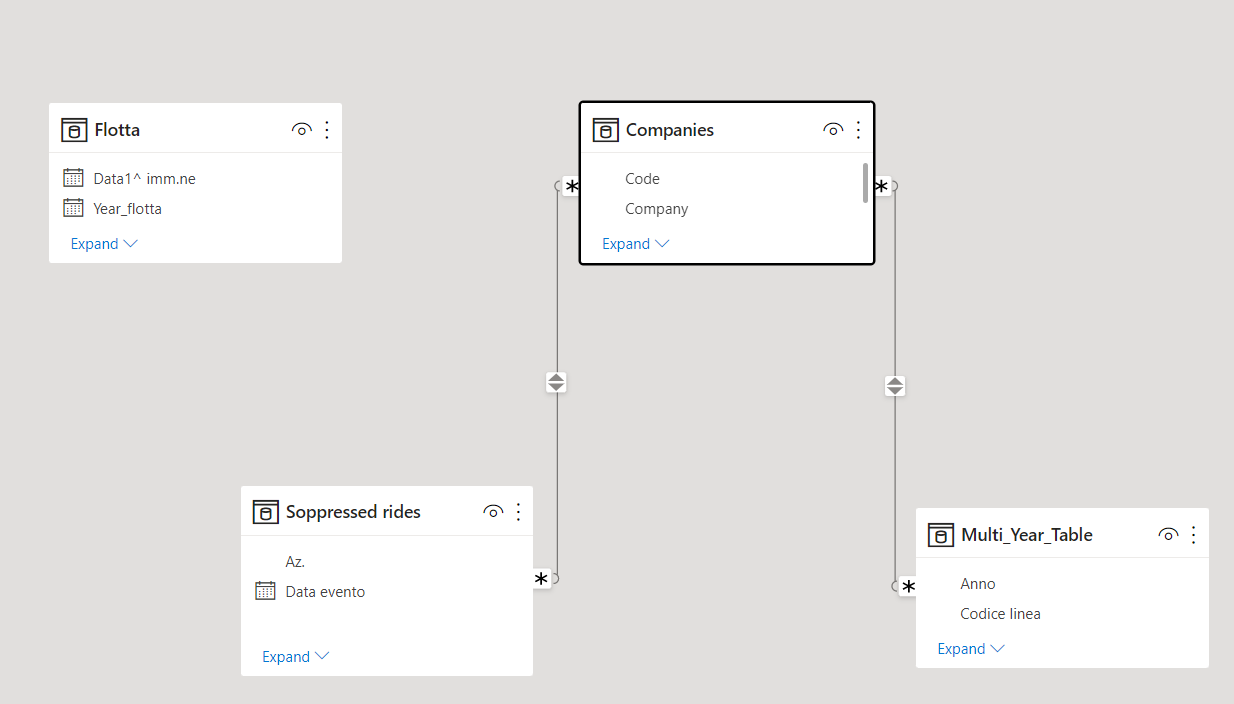
\includegraphics[width=0.9\textwidth]{Images/traditional_dashboard/ER_model.png}
    \caption{ER model of the Dashboard}
    \label{fig:ER}
\end{figure}
\section{Dashboard}

Starting from these tables, a dashboard is designed. It will be divided in subcategories that differ each other for the topic shown. In particular, the themes approached are:
\begin{itemize}
\item Suppressed rides
\item Bus requirements
\item Operative performances
\item KPIs correlation
\item Economics
\end{itemize}
\subsection{Suppressed rides}
In figure \ref{fig:sup} has been presented the dashboard.
\newpage
\WarningsOff
\begin{landscape}
\thispagestyle{empty}
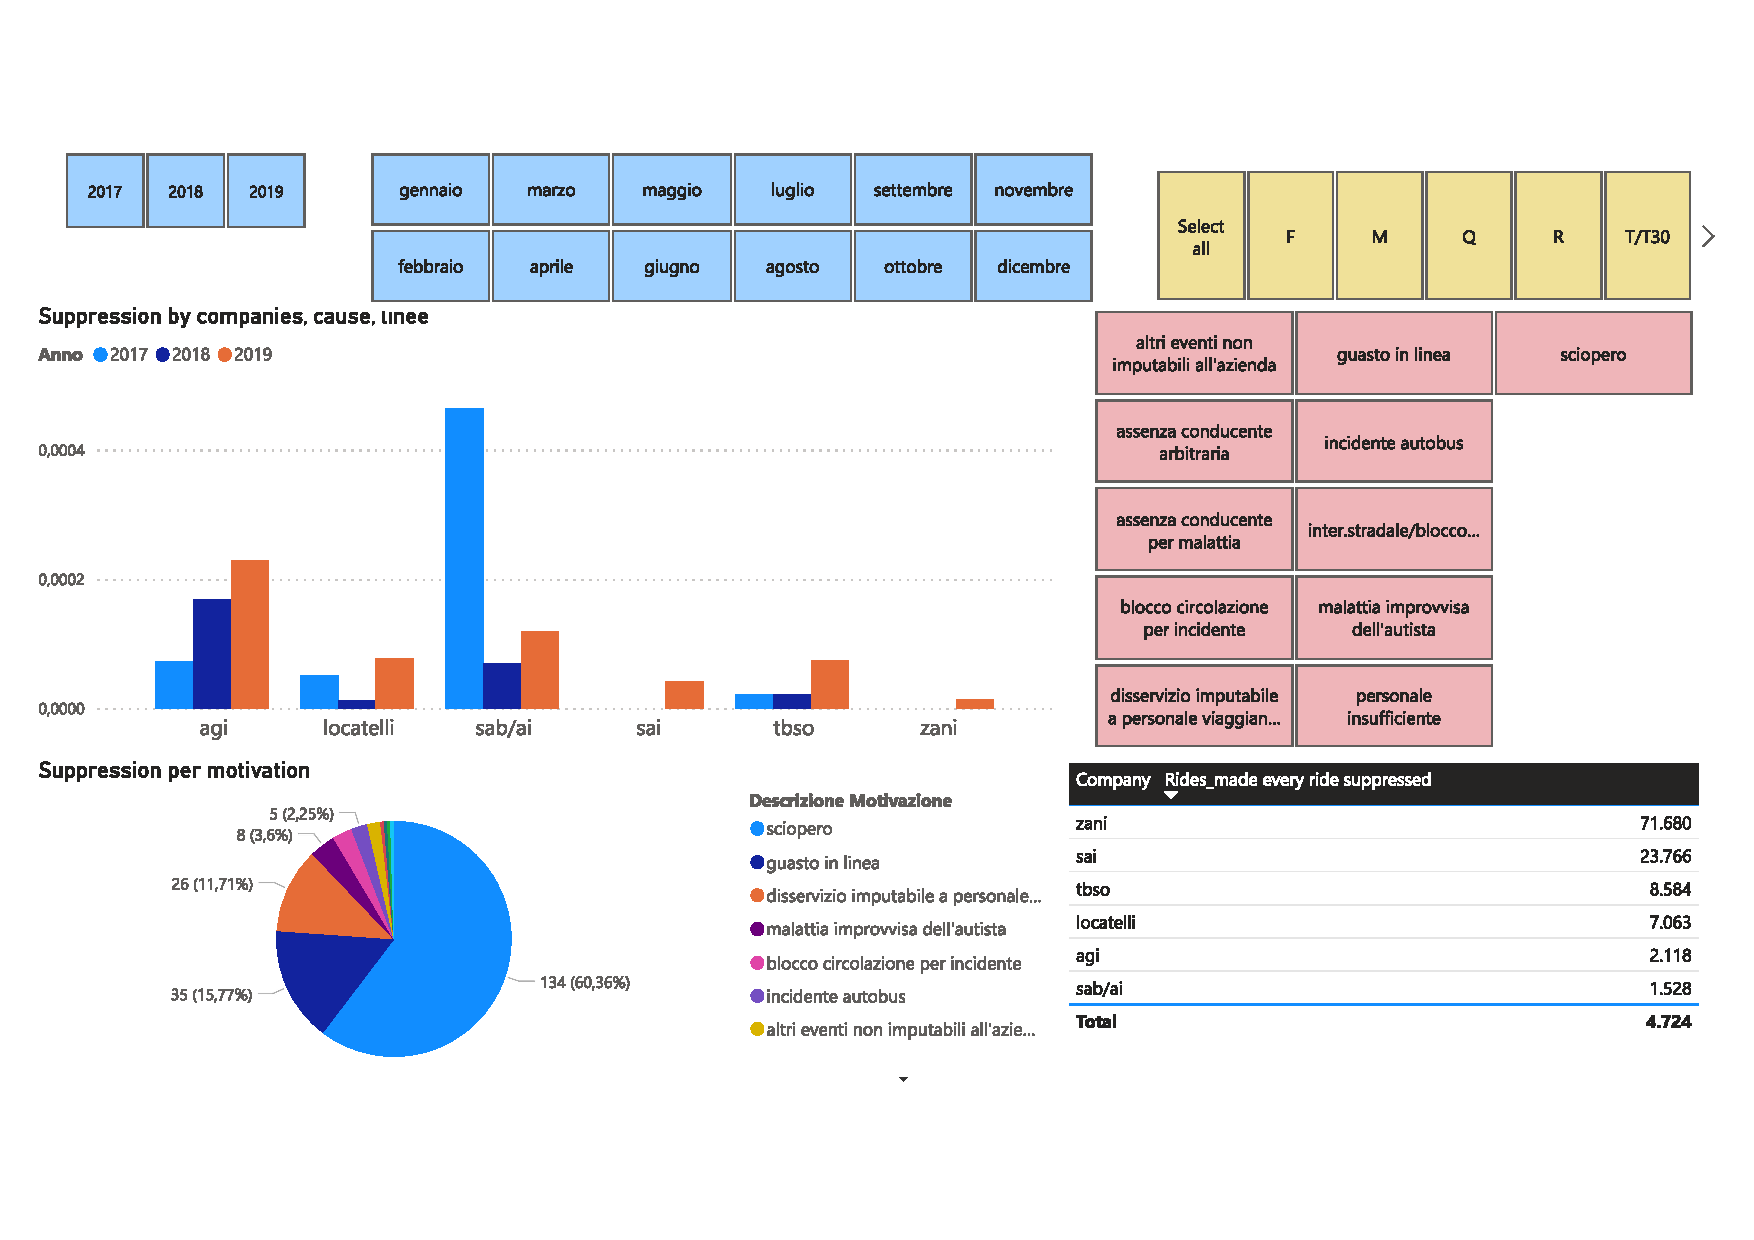
\includepdf[angle=90, pagecommand={\null\enlargethispage{2\baselineskip}\vfill\captionof{figure}{Suppressed}\label{fig:sup}}]{dashboard/Suppression.pdf}
\end{landscape}
\newpage
As said before, data about suppressed rides are between 2017 and 2019. An area of this part of the page is dedicated to filters, thanks to which data can be visualized according to:
\begin{itemize}
\item  period of time with a level of detail equal to a month
\item line
\item reason for which the ride was suppressed
\end{itemize}
Obviously, these filters could be used at the same time in order to obtain very specific analysis.

The table on the bottom right shows the number of rides traveled per each ride suppressed for each company. So, a low number corresponds to a bad result for the company. This data is computed in a relative way in order to show if a company has bad performances according to its dimension. A ride suppressed for a small company is not comparable with few rides suppressed for a big one. 

The pie chart has the goal of showing how the different causes affects suppressed rides, while the histogram shows the total suppressed rides for each year divided by company. 

Considering the dashboard without applying any filter, some considerations can be already done. In 2017 Sab/ai had a huge issue with suppressed rides that reached a percentage level double than the second highest one, in the analyzed period. In 2017 and 2018 Sai and Zani had no problems and their suppressed rides were equal to zero. Finally, Agi had a ever increasing problem related to suppressed rides. 

Moreover, the main cause that brings to a suppressed ride is strike followed at a distance by failure happened during service and inconvenience due to drivers during service. 

Finally, companies with performances below Consortium average are Agi and Sab/ai with, respectively, a ride suppressed every 2,118 and 1,528 rides traveled. 

\newpage

\begin{landscape}
\thispagestyle{empty}
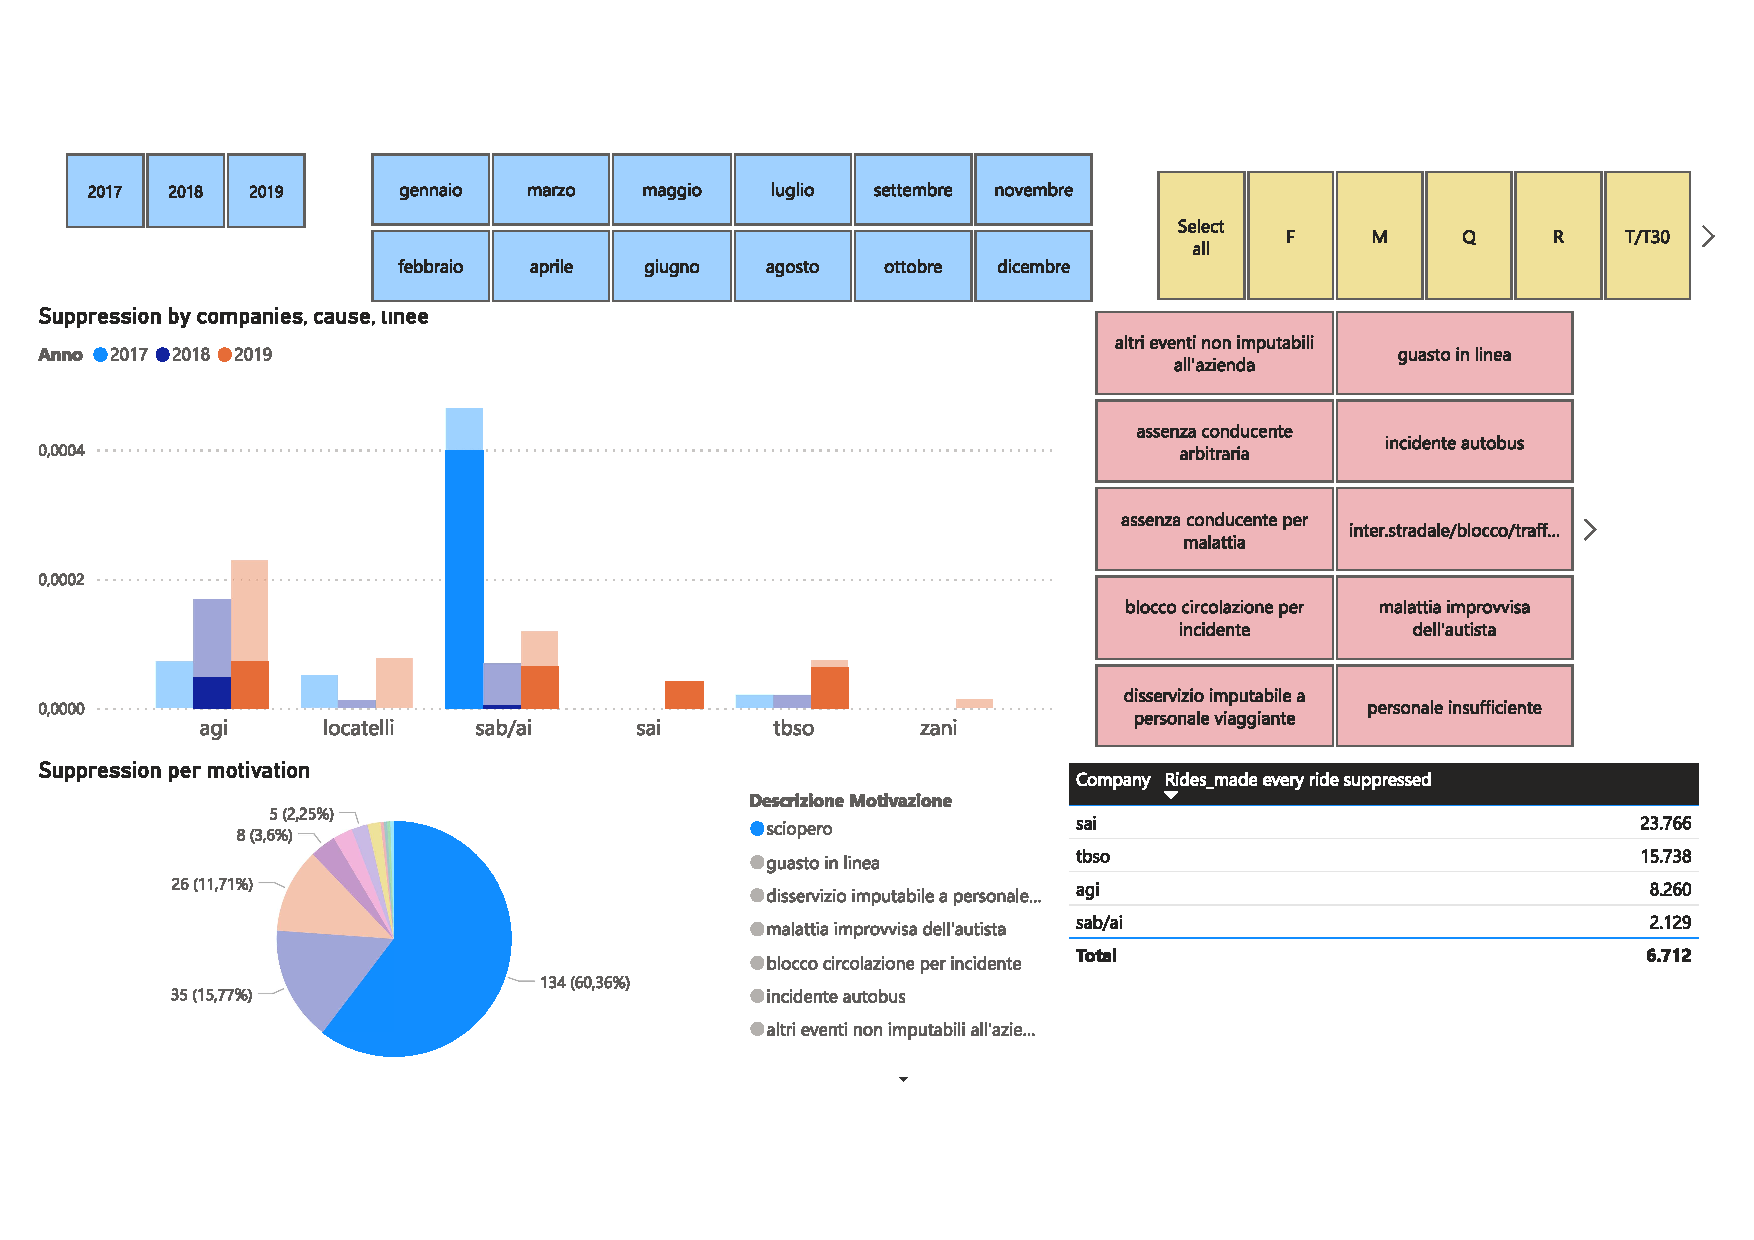
\includepdf[angle=90,  pagecommand={\null\enlargethispage{2\baselineskip}\vfill\captionof{figure}{Suppressed for strikes}\label{fig:strikes}}]{dashboard/Suppression_for_strikes.pdf}
\end{landscape}
\newpage

A focus on the strikes, shown in figure \ref{fig:strikes}, gives several information. Strikes are the reason of the abnormal problems tha Sab/ai had in 2017, moreover a strike in 2019 hit almost every company in an equal measure and, finally, Agi growing issues during this period are reflected also in strikes trend. 

Filtering data according to failure happened during service, a very interesting result is shown: half of the total failures happened during the three year in the Consortium happened during a ride performed by Agi even if Agi is one of the companies with less kilometers run per year. Moreover, this problem in absolute terms remains constant during the year and the negative trend of Agi is due to the increasing of other issues that in 2017 were almost absent.

\newpage
\begin{landscape}
\thispagestyle{empty}
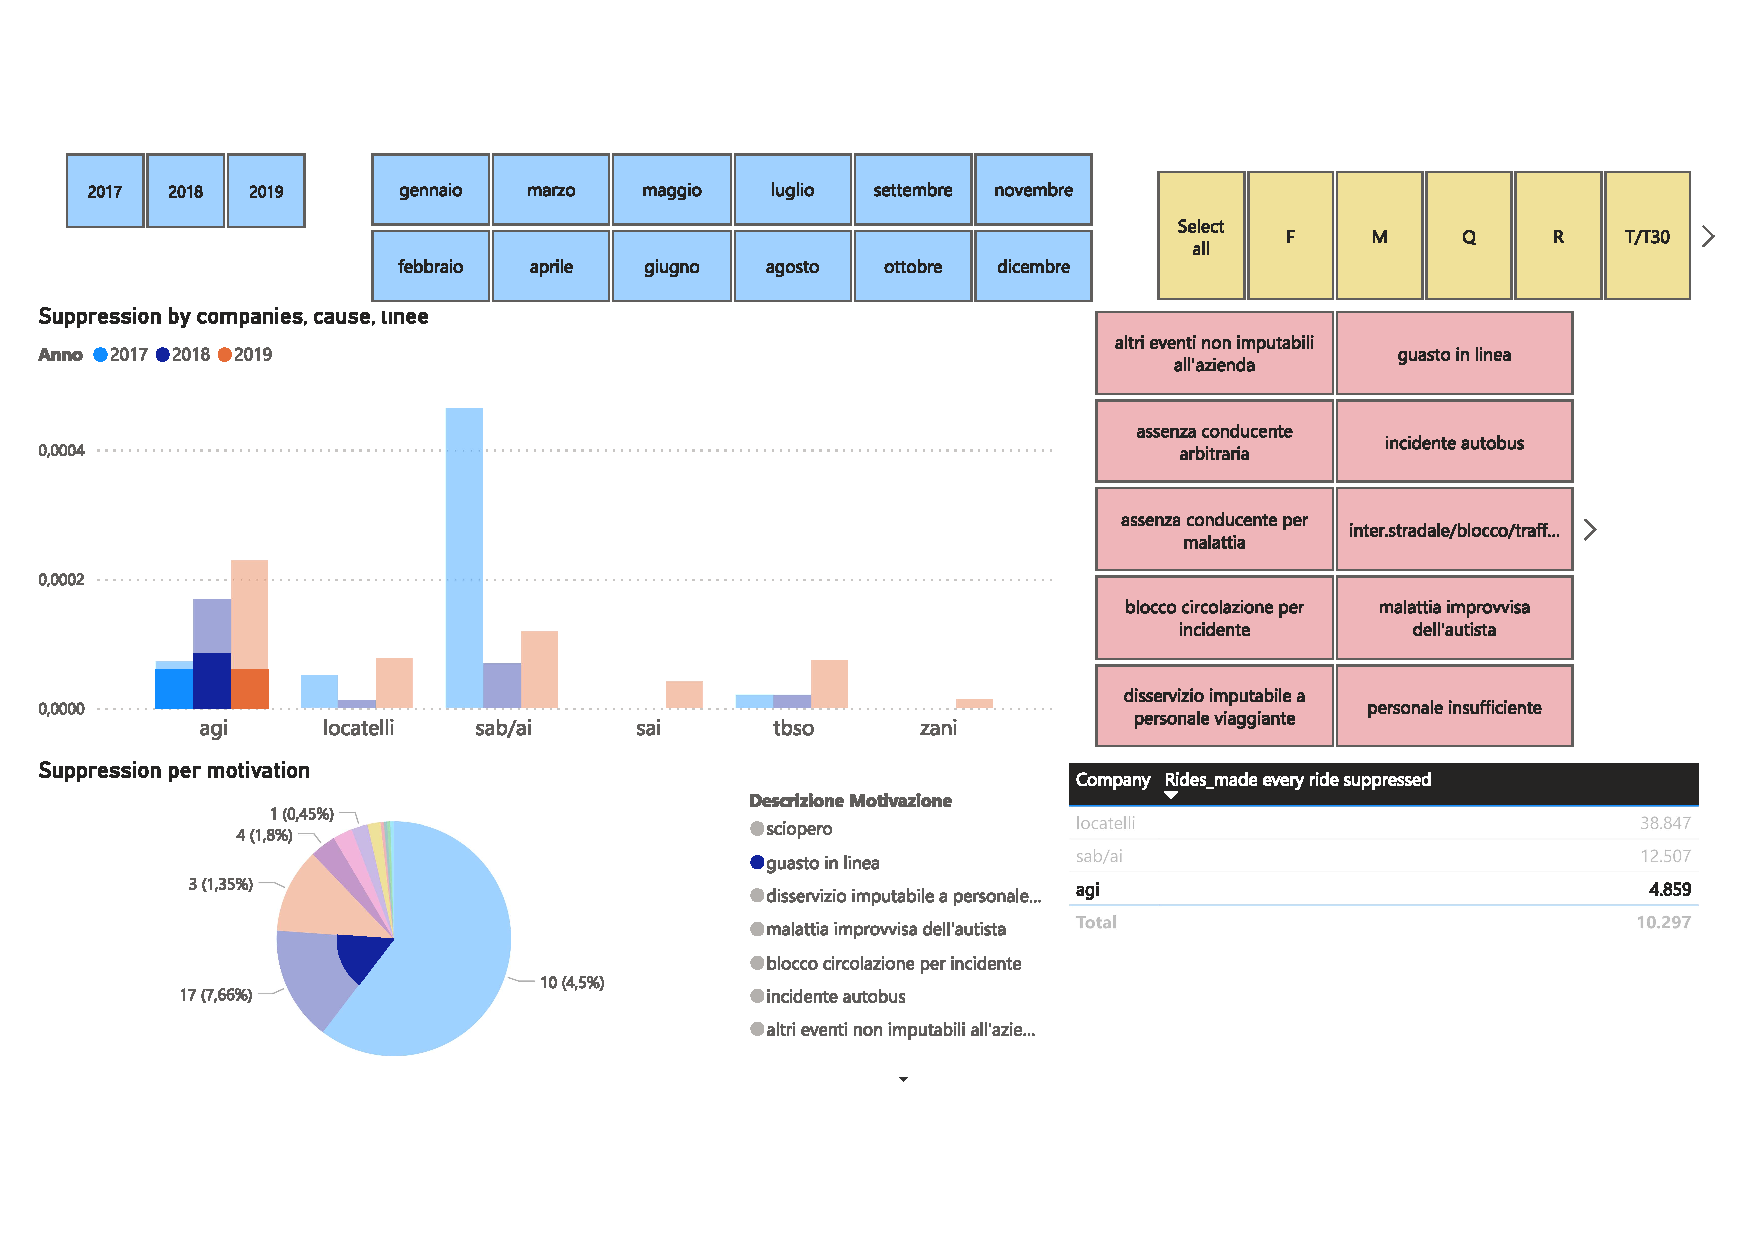
\includepdf[angle=90, pagecommand={\null\enlargethispage{2\baselineskip}\vfill\captionof{figure}{Focus on Agi and fault on the line}\label{fig:failline}}]{dashboard/Suppression_for_fail_on_the_line.pdf}
\end{landscape}
\newpage

\subsection{Fleet}

The second part of the dashboard regards an overview of the fleet based on the aspect that are underlined in the contract of service and that should be considered as constraint for a good fleet management, even if not all of them brings directly to a penalty from the Public Transport Authority. 

In particular, in the contract the PTA requires the following fleet criteria:
\begin{itemize}
\item $100\%$ buses must be air-conditioned
\item $91\%$ accessible for people with reduced mobility
\item  $100\%$ eco-diesel
\item at least $62\%$ Euro V, Euro VI, EEV or technologies with better emission performances.
\item  age restrictions:
    \begin{itemize}
        \item No restrictions if the age is lower of 18 years
        \item Travel limitation between 19 and 21 years, they can't be over $20\%$ of the total fleet
        \item Not allowed if they are over 22 years
    \end{itemize}
\end{itemize}
The figure \ref{fig:fleet}
shows the fleet situation in 2020, that is the most recent situation available. Data about 2018 and 2019 fleet are also available, so that comparison between these years can be done. Each aspect listed before is summed up in a pie chart that let a clear visualization of the situation.

Beginning from the good aspects, the entire fleet uses an eco-diesel fuel and almost every bus is equipped to allow the transport of people with reduced mobility. 

In Italy the average fleet age is about 12 years\cite{rossiPTM}, but in 2020 the Consortium results are even better with an average age of about 10 years. Despite this, 10 buses have an age that obliges them to suffer travel limitations and the $13\%$ in the immediate future will be in this situation. 

On the other side, as much as 8 buses are not equipped with air conditioning and, according to the contract of service, they should not travel. Finally, it is possible analyze the fleet according to their emission category. The requirements set by the contract ($62\%$) are widely satisfied, but the improvement margin is really high since the $30\%$ of the fleet has an high polluting engine. 


\newpage
\begin{landscape}
\thispagestyle{empty}
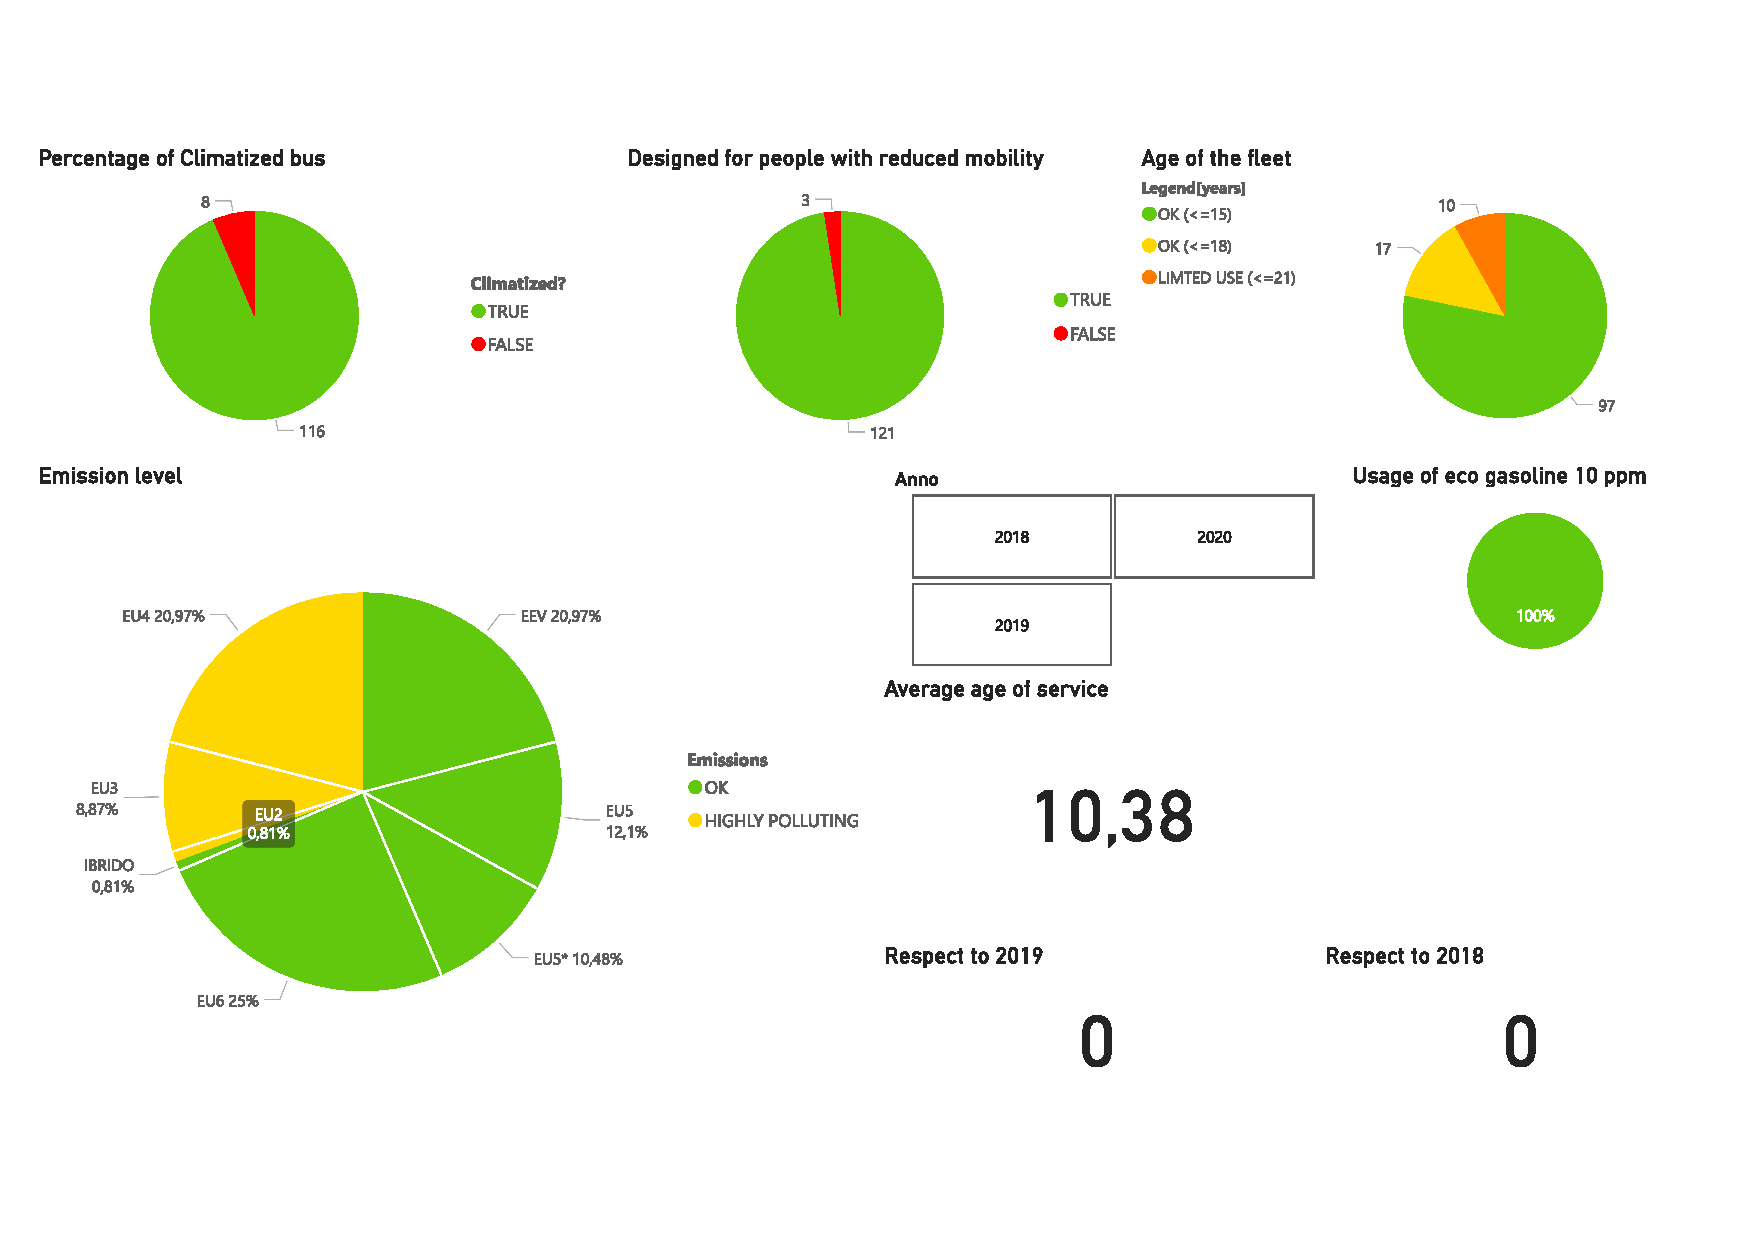
\includepdf[angle=90, pagecommand={\null\enlargethispage{2\baselineskip}\vfill\captionof{figure}{Fleet dashboard}\label{fig:fleet}}]{dashboard/emission.pdf}
\end{landscape}
\newpage

In the figure \ref{fig:fleetold}  a focus on the oldest part of the fleet in 2020, the one that has constraint on traveled kilometers. 

It can be seen that the majority of those buses are also the ones that are not air-conditioned, so, if they are replaced with new ones, two bad situations can be improved . Moreover, two of the three buses not equipped for people with reduced mobility belongs to this category. Unfortunately, if they are removed, an important percentage of not polluting buses would be lost. In fact, the $5\%$ of the fleet is composed of old buses with a swapped engine in order to respect contract limitations. Finally, the presence of buses with an age over 17 years is really increased respect to 2018, with a rise of over $200\%$.


The third dashboard (figure \ref{fig:fleetinquinanti}) is a focus on the most polluting part of the 2020 fleet, so buses with Euro 3 and Euro 4 standard technology. Fortunately, the majority of them has the less polluting engine, symptom of good turnover of the fleet during the previously years. Theoretically, their presence in the fleet is not against the rules written in the Service Contract, but from a modern point of view, they could be a stain in terms of sustainability and green attitude. In particular, in this dashboard an analysis about the newest subpart of fleet, the buses under 15 years, is performed. This focus is motivated by the fact that, despite their polluting nature, according to the contract, these buses could travel for many years (at least 6) on Bergamo province streets. So, these buses are all air-conditioned and designed for people with reduced mobility. Despite the set constraint of an age under 15 years, their average age is really high, 14 years, showing that their matriculation happened in a small period of time. Moreover, their decrease is consistent and regular in the last years and this shows a huge presence among buses that have not yet contractual restrictions. This last consideration is confirmed by the previous dashboard. Since this part of the fleet has several years in front of it and since its characteristics respect all the contract requirements, a suggestion could be an engine swapping with a less polluting standard then an expensive turnover of the entire fleet, or better, a mix of the two solutions.
\newpage
\begin{landscape}
\thispagestyle{empty}
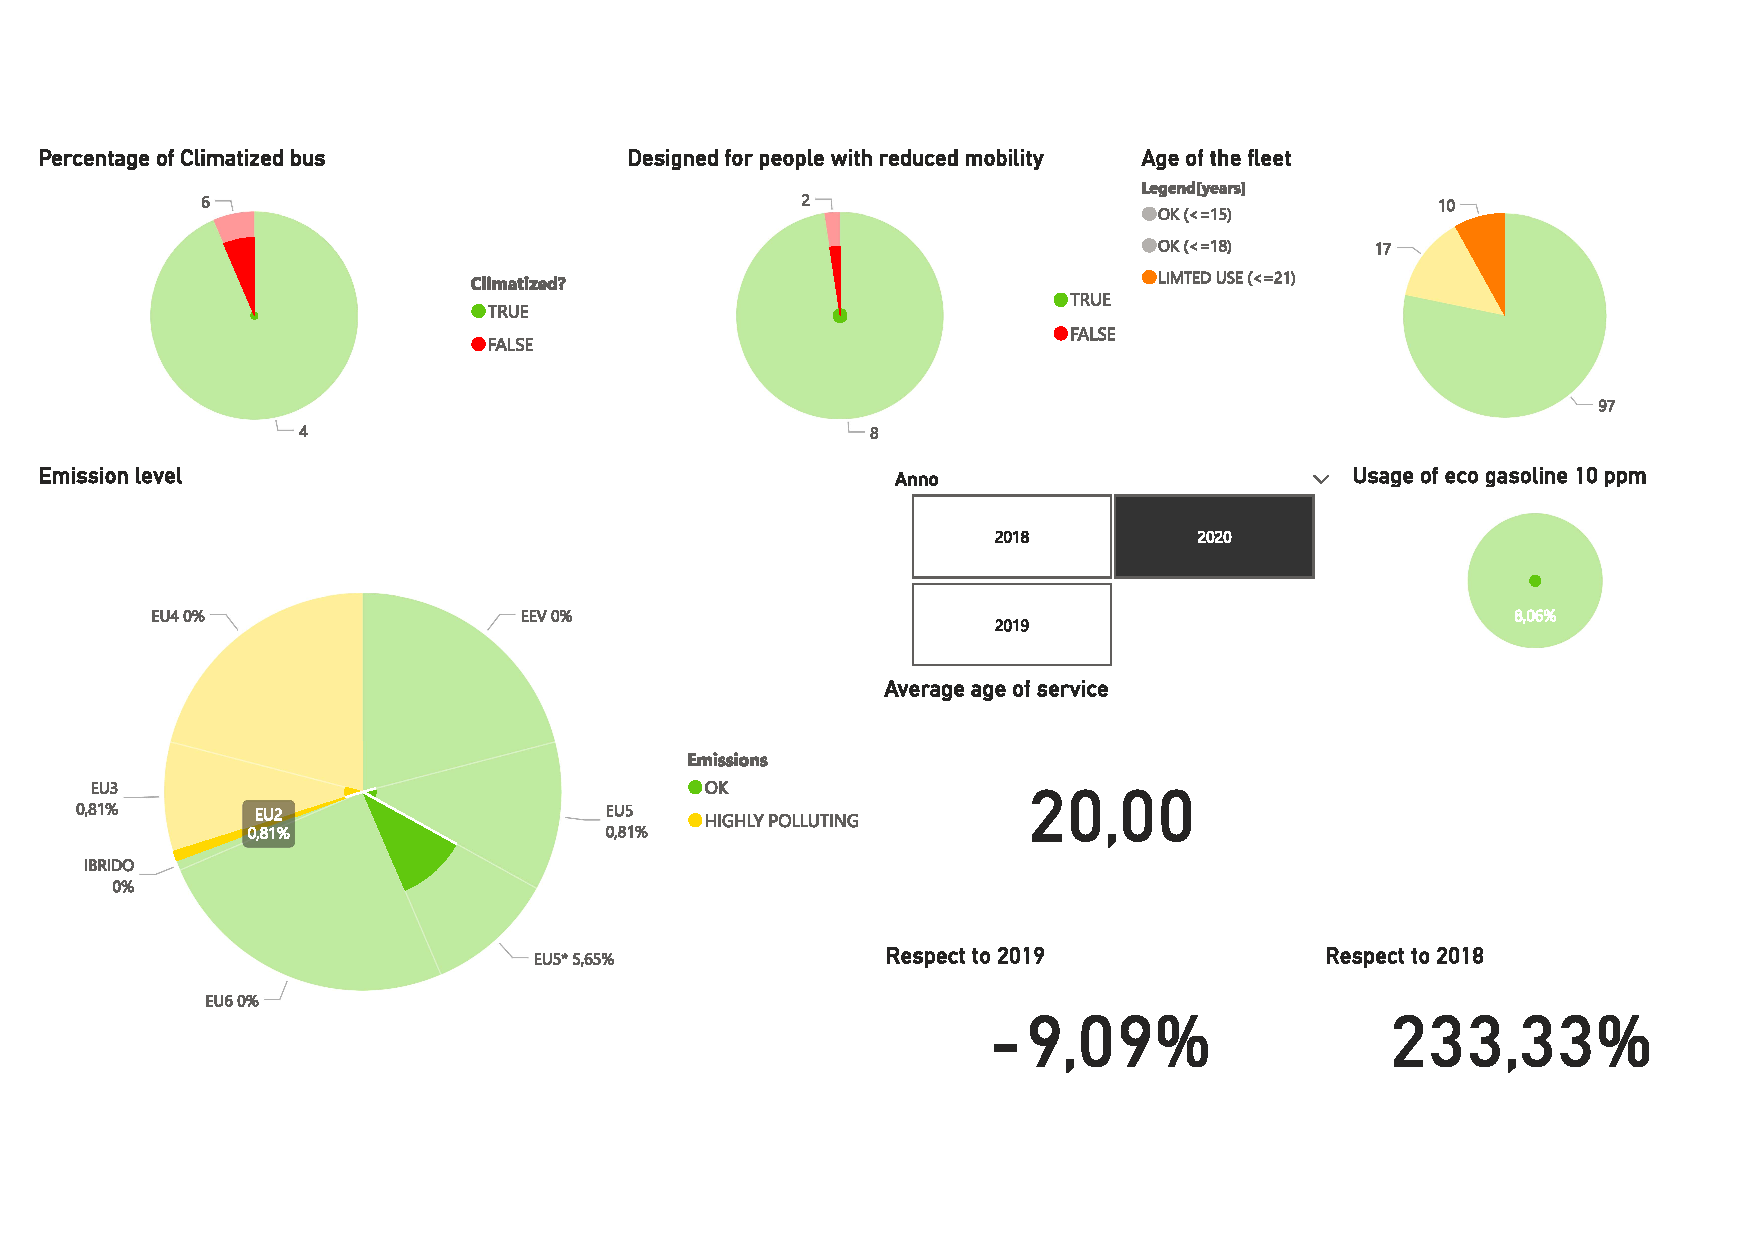
\includepdf[angle=90, pagecommand={\null\enlargethispage{2\baselineskip}\vfill\captionof{figure}{Focus on old fleet}\label{fig:fleetinquinanti}}]{dashboard/fleet_old_2020.pdf}
\end{landscape}
\newpage


\newpage
\begin{landscape}
\thispagestyle{empty}
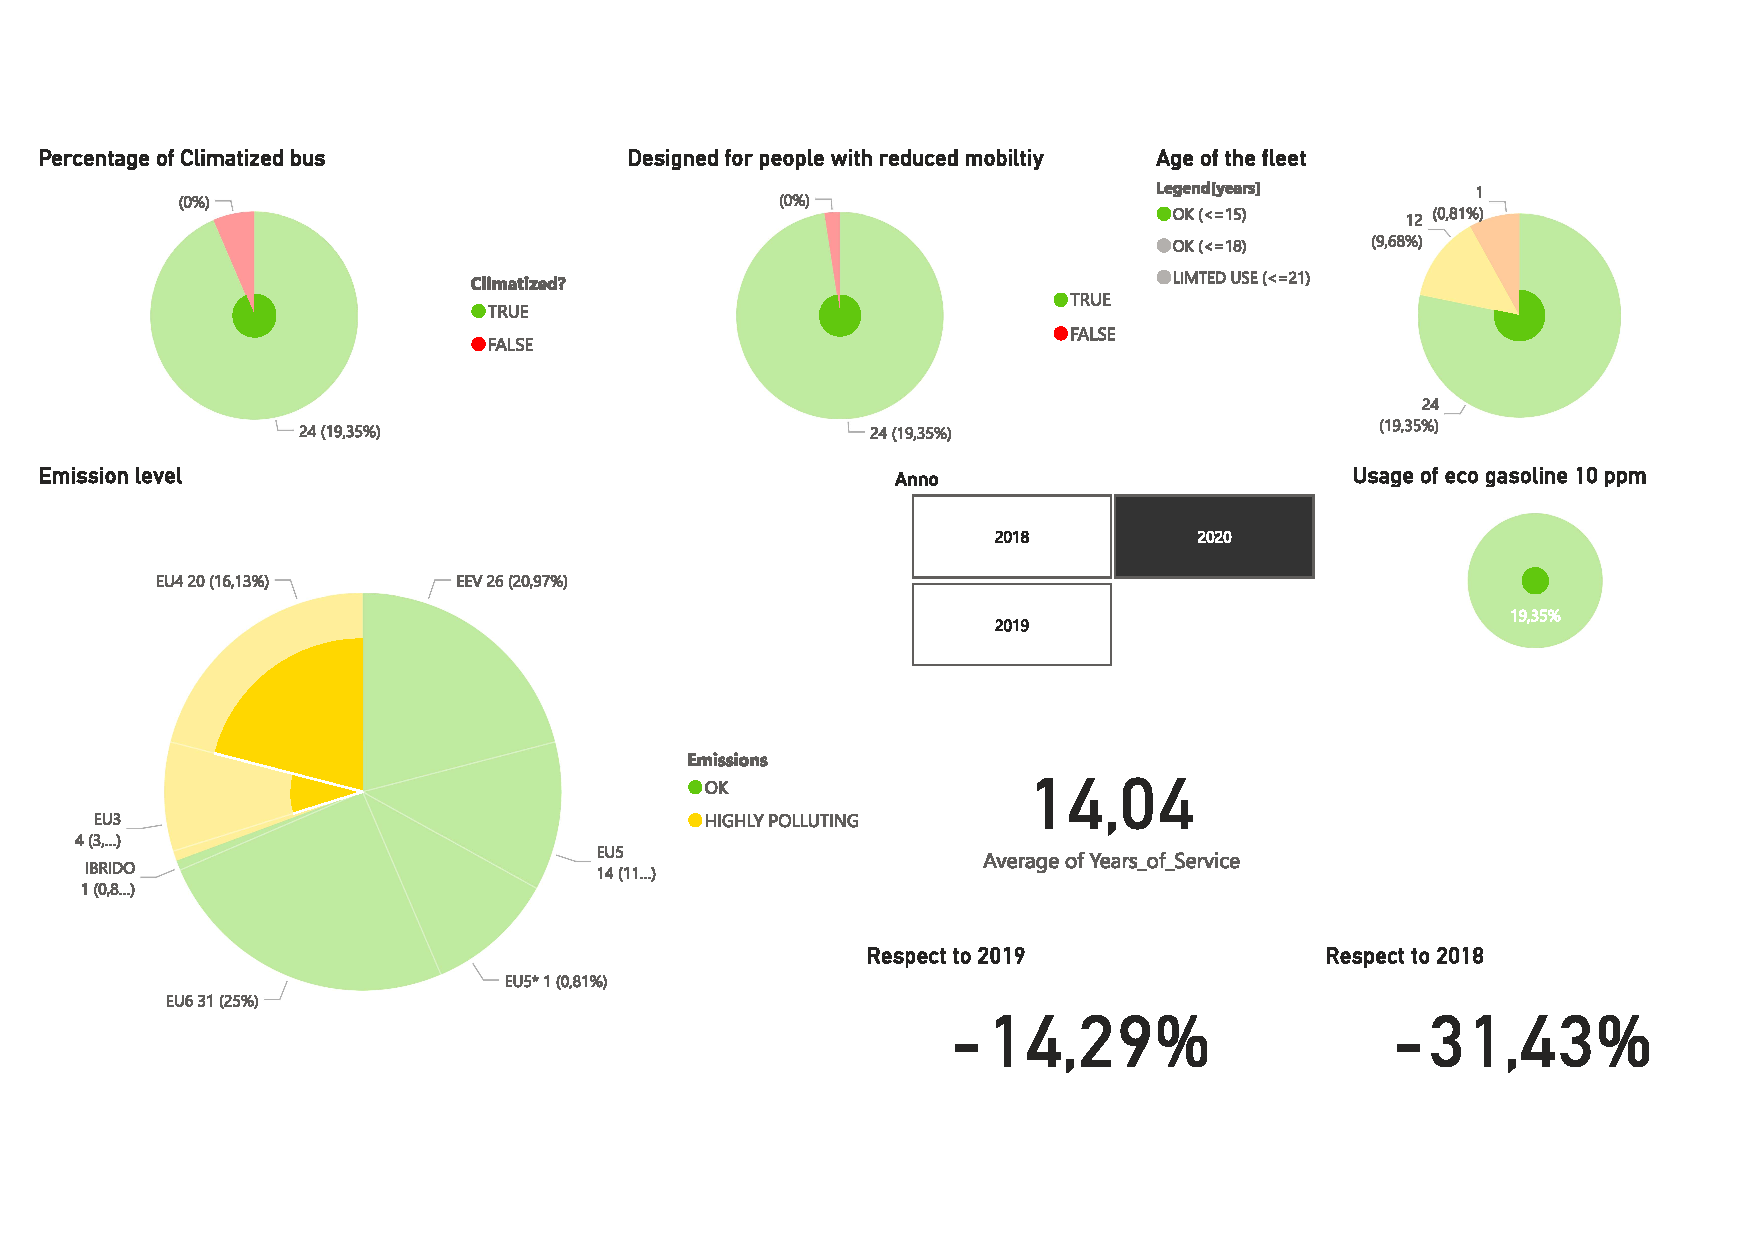
\includepdf[angle=90, pagecommand={\null\enlargethispage{2\baselineskip}\vfill\captionof{figure}{Focus on old fleet}\label{fig:fleetold}}]{dashboard/fleet_inquinanti.pdf}
\end{landscape}
\newpage

\subsection{Operative performances}
The aim of this page is to present the ratio of rides made by the companies of the consortium. 

In the bottom part of the figure \ref{fig:op} there are two filters that allow the selection of Lines and Years.

Above them,  the average of the percentage of rides made by the companies\footnote{the reader can argue that some of the companies has a percentage of ride made up to $100\%$ but they had suppression in the previous page. This is due to the fact that the quantity of suppression is very low with respect to the rides made each month by the companies. For this reason in the data can have been approximated}. Moreover, these data include 2020 and 2021, so companies with good performances before could have suffered diseases due to Covid-19. On the right, the commercial speed divided by lines is shown.

Finally, on the top the correlation between the average percentage of rides made and the commercial speed per companies.

With only this view can been seen four cluster of companies:
\begin{itemize}
    \item \textbf{sai} and \textbf{tbso} that has less than 28 km/h
    \item \textbf{locatelli} near 30 km/h
    \item \textbf{arriva}, \textbf{zani} around 35 km/h
    \item \textbf{agi} that are above 38 km/h 
\end{itemize}
This result, if combined with the timetable of the service (not provided) can help to find the company with the better performances. With the information provided can not be sure that agi is the member with better performance because it depends on the route that agi buses travel and on the time in which it operates. 



\newpage
\begin{landscape}
\thispagestyle{empty}
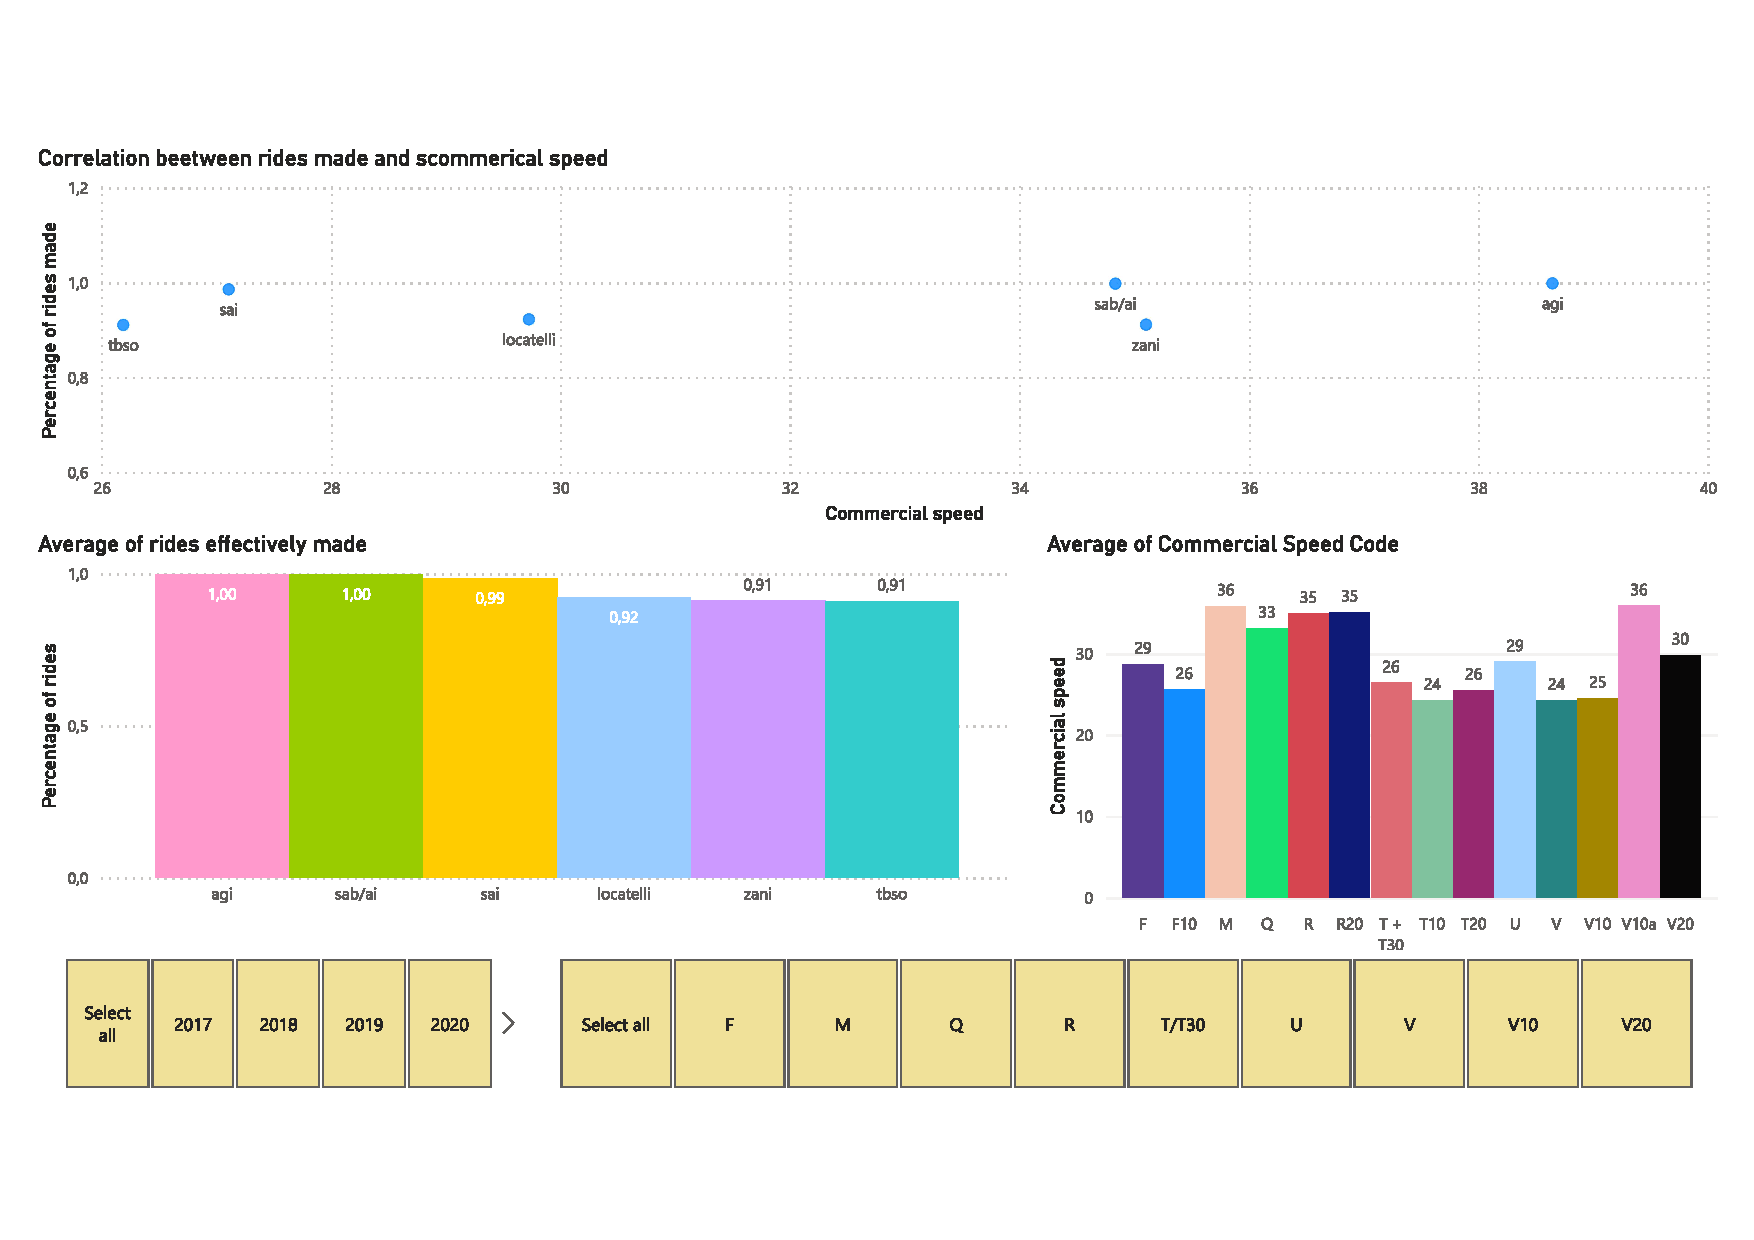
\includepdf[angle=90, pagecommand={\null\enlargethispage{5\baselineskip}\vfill\captionof{figure}{Operativ performances}\label{fig:op}}]{dashboard/operative_performances.pdf}
\end{landscape}
\newpage

\subsection{KPIs Correlation}
The page represented in \ref{fig:corr} contains the relationships between:
\begin{itemize}
  \item the cost and the income
   \item the ratio I/C and the the commercial speed
    \item ratio I/C and the suppression
\end{itemize}
From cost-income graph, it is clear that Tbso has the worst economic situation because it spends a considerable amount of money per km, even if their introits are the lowest ones. For a better clearness, the median of costs and incomes is drawn.

For the other two graphs, the ratio between income and cost is set as symbol of efficiency. With this hypothesis, it is possible to plot the relationship with suppressed rides and commercial speed in order to see if these two factors have influences on the performances of the companies. 

The graph with the commercial speed as x-axis is emblematic. Excluding Sai that seems to be an outlier for its very good efficiency, despite its low commercial speed, for the other companies the correlation is striking: higher the speed is, better the economic efficiency is. 

On the other side, the same thing can not be said for the suppressed lines. They do not seem to cause any issue to economic performance, indeed the companies that suffer more this problem are also the most efficient.

Unfortunately, this kind of dashboard is difficult to deepen if this characteristics are maintained. It could be more interesting evaluating the single lines, since they are more influenced on aspect such as commercial speed. From figure \ref{fig:corrlines} for example, it is evident that not all the lines traveled by Tbso have high cost, but only V10. This should lead the company to work on understanding the problems that this line creates. On the other side, line V20, always under Tbso management, has incredibly bad performances about incomes. 

The two lines that indicate the median cost and the median income become useful to divide the lines in four categories:
\begin{enumerate}
\item The best: high income, low cost
\item The satisfactory: high income, high cost
\item The improvable: low income, low cost
\item The worst: low income, high cost
\end{enumerate}
The lines that belong to the last category are the aforementioned line V10 and line F (Bergamo - Treviglio). 
On the other side, the best performances are obtained by line V, and this is curious because its underlines V10 and V20 have huge problems, line R (Bergamo - Soncino) and line U (Bergamo - Treviglio). 

It is interesting that the correlation between commercial speed and economic efficiency disappears when the situation is analyzed considering the single lines. Probably, since some lines are managed by more than one company, the society that controls the service has a big impact on the economic performances.

Focusing on 2020, a disastrous year for the transport sector, it is possible to notice that the efficiency of each line is stable, without any substantial difference determined by commercial speed. This could be a symptom of Covid-19 that hit equally every companies. The graph on the right shows that the median of incomes slightly decreased, while the median of costs considerably increased respect to the three-years period 2017/19 of the previous dashboard. In order to have a clearer idea of the performances, a comparison of the selected year with the two years before can be seen. In 2020, the disaster is evident. The costs grew by 13$\%$ respect 2019, probably because the higher incidence of fixed costs, but the dramatic data is about incomes that dropped by 35$\%$. Consequently, the efficiency decreased by 42$\%$. An interesting aspect is that the commercial speed did not rise hugely, despite of the lockdown period in which streets were empty. 

\newpage
\begin{landscape}
\thispagestyle{empty}
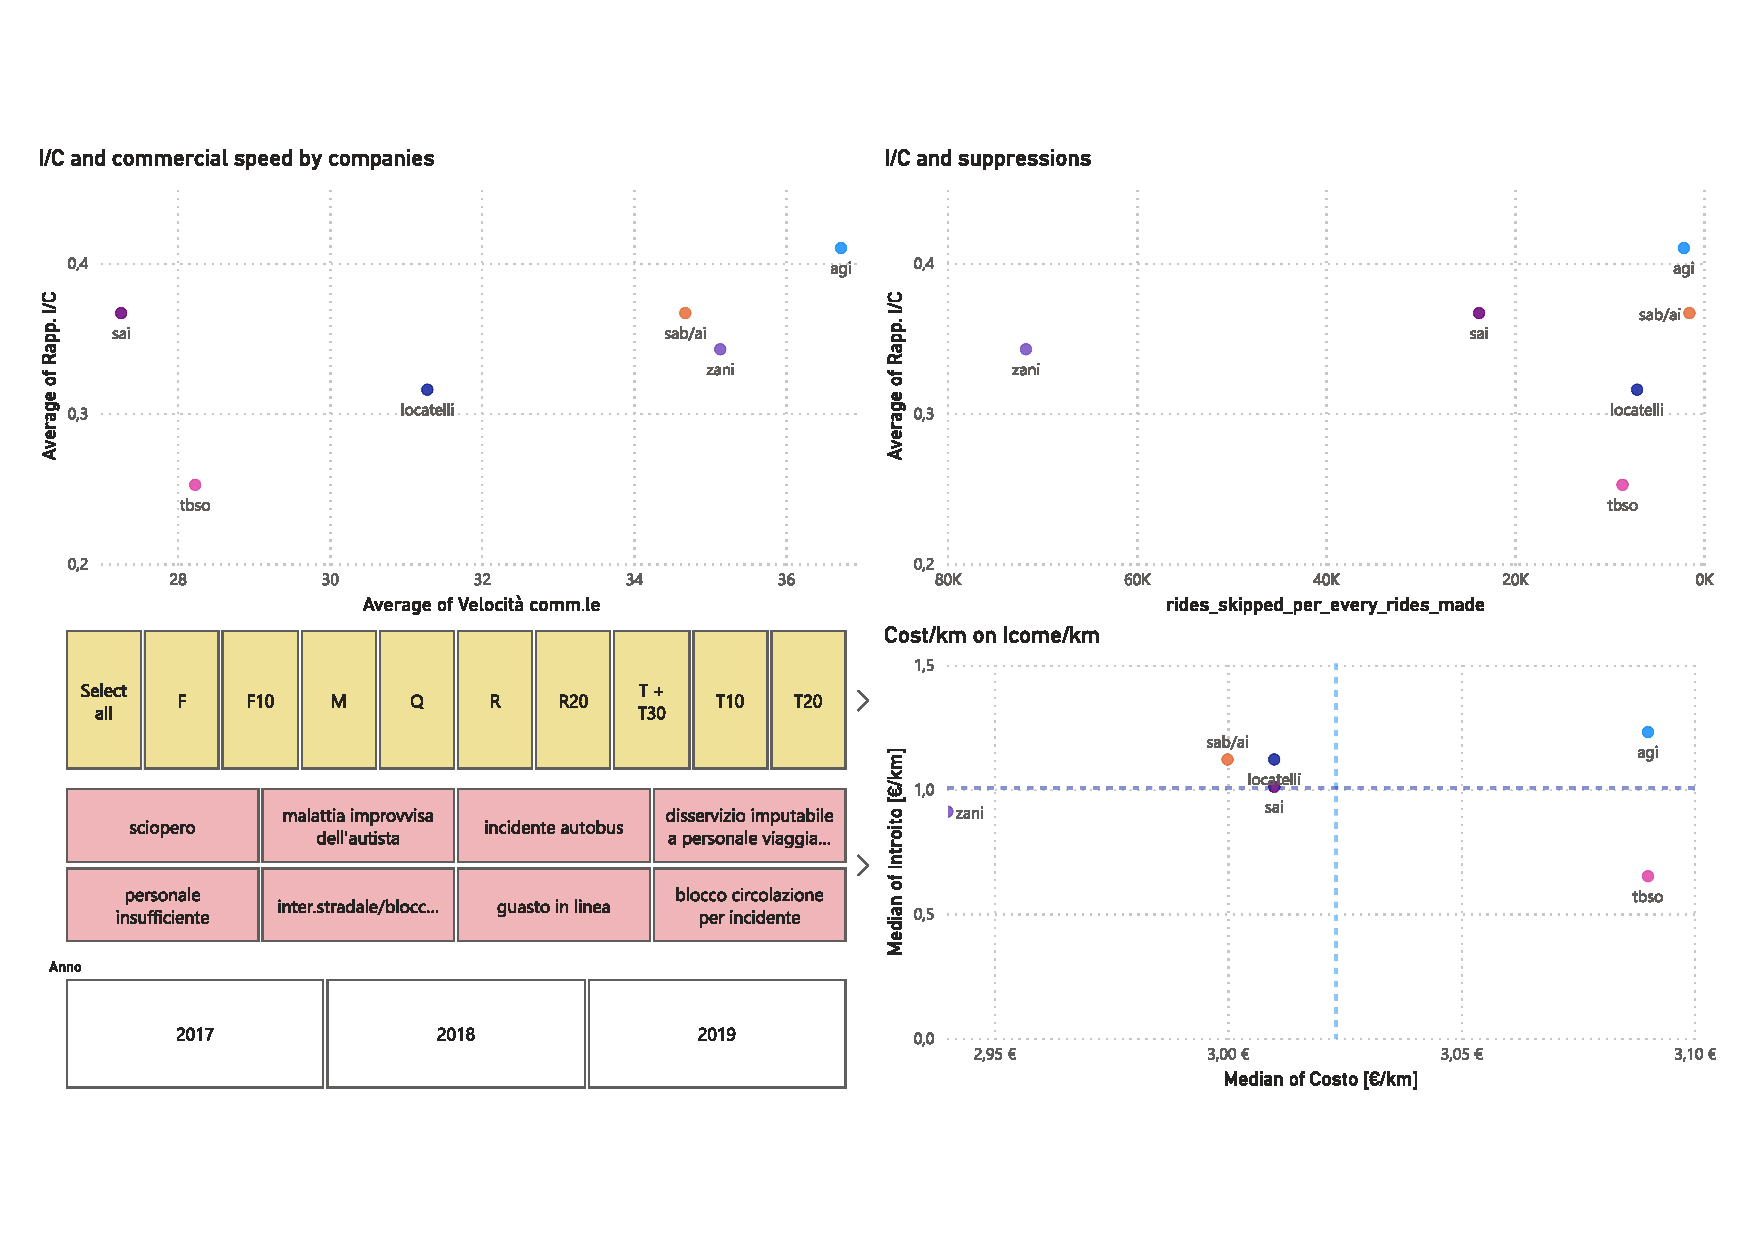
\includepdf[angle=90, pagecommand={\null\enlargethispage{3\baselineskip}\vfill\captionof{figure}{Page about correlation}\label{fig:corr}}]{dashboard/correlation.pdf}
\end{landscape}
\newpage


\newpage
\begin{landscape}
\thispagestyle{empty}
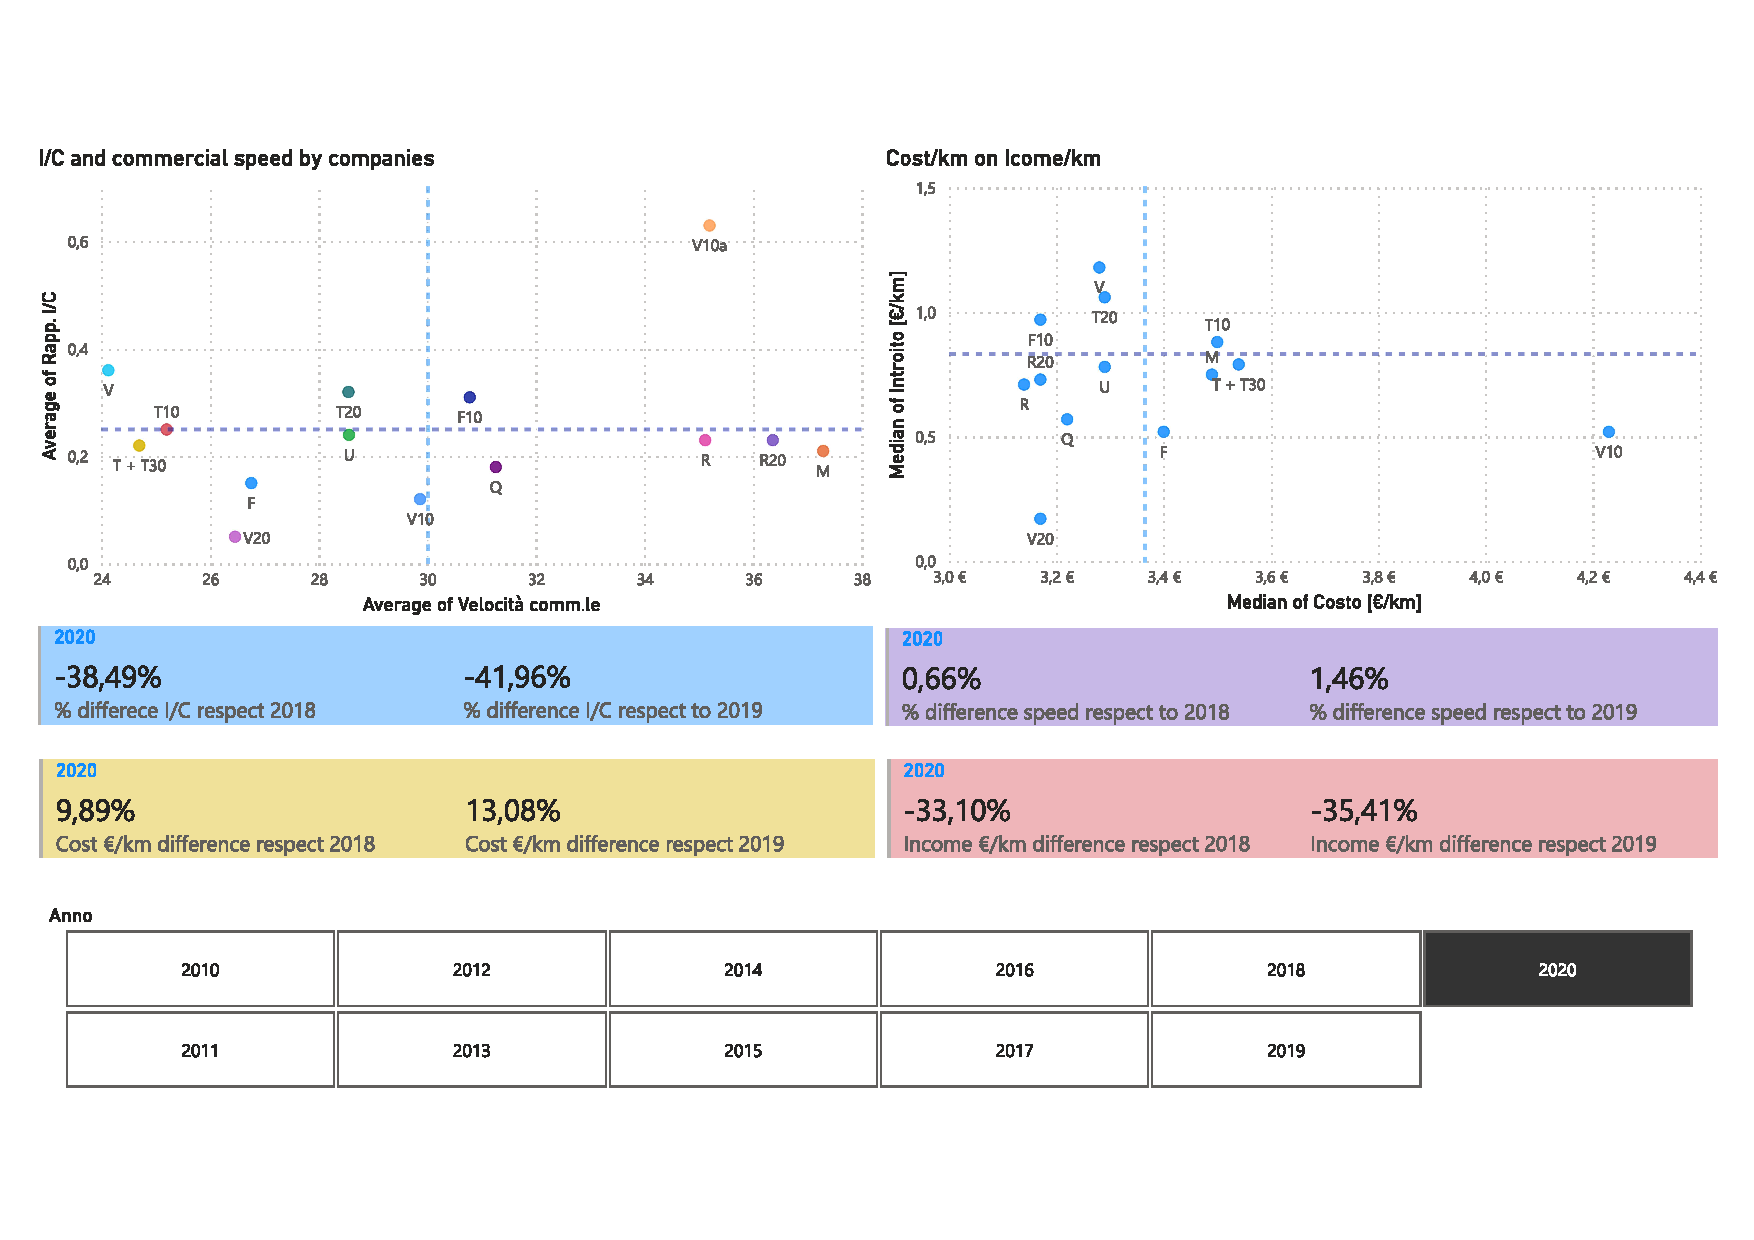
\includepdf[angle=90, pagecommand={\null\enlargethispage{3\baselineskip}\vfill\captionof{figure}{Percentage difference}\label{fig:corrlines}}]{dashboard/correlation_2.pdf}
\end{landscape}
\newpage
\begin{landscape}
\thispagestyle{empty}
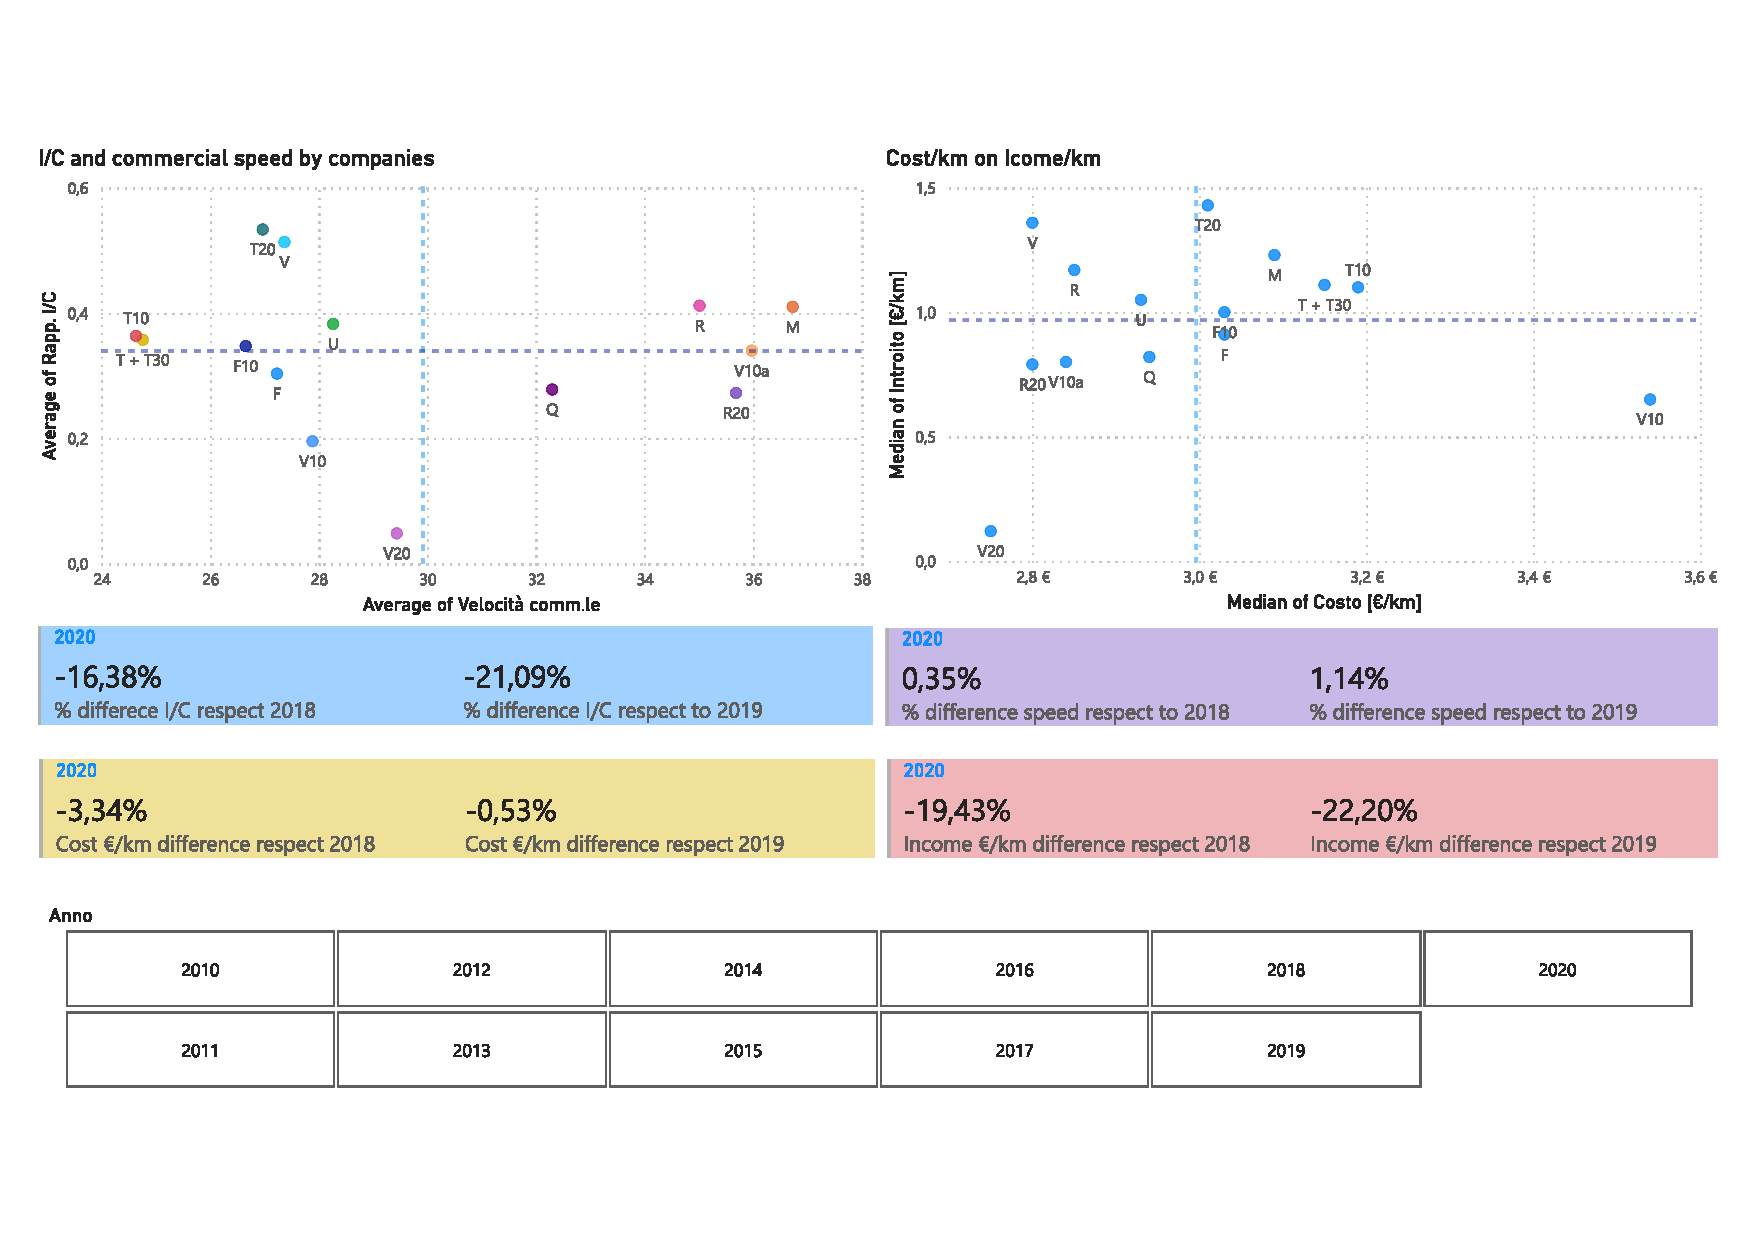
\includepdf[angle=90, pagecommand={\null\enlargethispage{3\baselineskip}\vfill\captionof{figure}{Percentage difference}\label{fig:corrlines2}}]{dashboard/correlation_without_year.pdf}
\end{landscape}

\subsection{Income}
The last part of the dashboard is about a large picture of the economic situation. The screenshot that is shown at the following page \ref{fig:income} is one of the many example in which this kind of graph could be shown. It shows the economic efficiency of the entire Consortium in the last 10 years, but then it focuses on the performances of a set of lines and finally it shows their situation in the desired period. In the example, a spotlight on Arriva situation. Arriva manages three lines: M (Bergamo - Crema), Q (Bergamo - Chiari) and R (Bergamo - Soncino). Two of them, M and R have performances above the average, while line Q has serious problems in economic efficiency. Finally, a focus on line M shows that the economic situation on that line is slowly improving. 

On the right side of the page, two graphs about incomes and costs per kilometer in the last decade. In particular the ones in the figure \ref{fig:income} refer to M line. The graphs evidence that the increasing economic efficiency of this line happened because of a constant incomes growth, while, on the other hand, the costs were stable with a drop in 2014. The 2020 disaster is confirmed once more by the dramatic decrease of incomes and the consistent increase of costs.
\newpage
\begin{landscape}
\thispagestyle{empty}
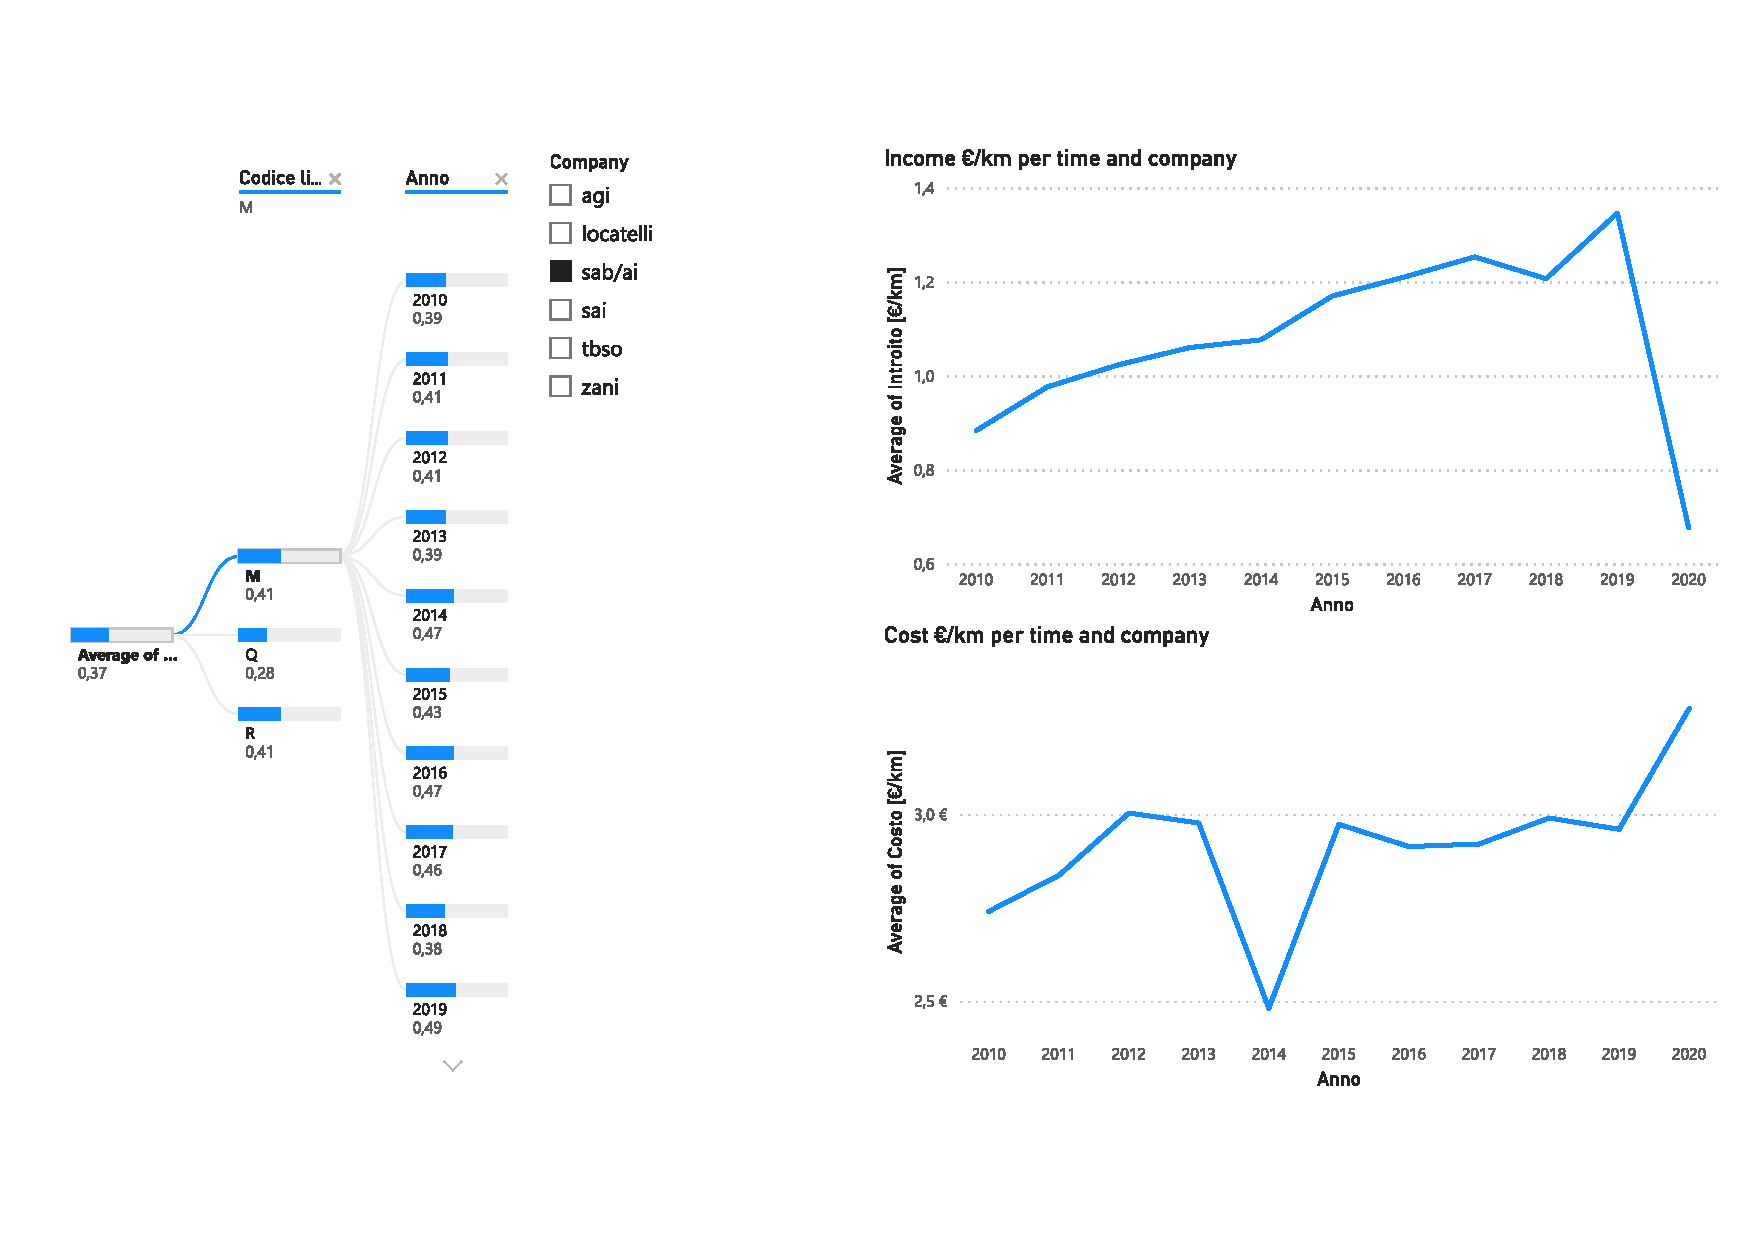
\includepdf[angle=90, pagecommand={\null\enlargethispage{2.5\baselineskip}\vfill\captionof{figure}{Percentage difference}\label{fig:income}}]{dashboard/income.pdf}
\end{landscape}
\WarningsOn
\chapter{Innovative KPIs}
\label{ch:Innovative}
\section{Introduction on the Innovative KPIs}
\label{sec:Intro_Innvovative}
In the last few years there is a growing interest in the concept of sustainability and sustainable transportation. New technologies and new objective to be achieved make it necessary to define new indicators to measure new relevant aspects related to sustainability.

The fundamental role of sustainable development is also confirmed by the 2030 Agenda for Sustainable Development, adopted by all United Nations Member States in 2015. It provides a shared blueprint for peace and prosperity for people and the planet, now and into the future. 

The 2030 Agenda defines \emph{17 Sustainable Development Goals (SDGs)}\cite{sdgs} referred to different areas of social, economic and environmental development and each goal has specific objectives to be achieved over the next few years. 

In the following table the 17 SDGs are reported the ONU target in 2030 and the respective sustainability topics that can be faced in a public transport company.

\newpage
\newpage

\begin{minipage}[c]{0.2\textwidth}
\centering
SDGs ONU
\end{minipage}
\fbox{
\begin{minipage}[c]{0.5\textwidth}
\centering
Target ONU 2030
\end{minipage}
}
\begin{minipage}[c]{0.2\textwidth}
\centering
LPT 
\end{minipage}


\begin{minipage}[c]{0.2\textwidth}
    
\includegraphics[width=\textwidth]{Images/Social_sustainability/1_no_poverty.png}
\end{minipage}
\fbox{
\begin{minipage}[c]{0.5\textwidth}
1.3 Apply at national level adequate systems and social protection measures for all, including minimum levels, and by 2030 achieve substantial coverage of the poor and vulnerable
\end{minipage}
}
\begin{minipage}[c]{0.2\textwidth}
\emph{Corporate welfare}
\end{minipage}


\begin{minipage}[c]{0.2\textwidth}
    
\includegraphics[width=\textwidth]{Images/Social_sustainability/3_helth.png}
\end{minipage}
\fbox{
\begin{minipage}[c]{0.5\textwidth}
3.8 Achieve universal health coverage, including protection from financial risks, access to essential quality health care services and access to safe, effective, quality and affordable essential drugs and vaccines for all
\end{minipage}
}
\begin{minipage}[c]{0.2\textwidth}
\emph{Corporate welfare}
\end{minipage}

\begin{minipage}[c]{0.2\textwidth}
    
\includegraphics[width=\textwidth]{Images/Social_sustainability/white_box.png}
\end{minipage}
\fbox{
\begin{minipage}[c]{0.5\textwidth}
3.6 By 2020, halve the number of deaths and injuries from road traffic accidents worldwide
\end{minipage}
}
\begin{minipage}[c]{0.2\textwidth}
\emph{Health and safety}
\end{minipage}

\begin{minipage}[c]{0.2\textwidth}
    
\includegraphics[width=\textwidth]{Images/Social_sustainability/4_education.png}
\end{minipage}
\fbox{
\begin{minipage}[c]{0.5\textwidth}
4.3 By 2030, ensure equal access for all women and men to affordable, high-quality education, vocational and third-level education, including university

4.4 By 2030, substantially increase the number of young people and adults who have the necessary skills, including technical and professional skills, for employment, decent work and entrepreneurial capacity

4.7 By 2030, ensure that all students acquire the knowledge and skills necessary to promote sustainable development through, inter alia, education for sustainable development and sustainable lifestyles, human rights, equality of gender, the promotion of a culture of peace and non-violence, global citizenship and the enhancement of cultural diversity and the contribution of culture to sustainable development
\end{minipage}
}
\begin{minipage}[c]{0.2\textwidth}
\emph{Training and\\ development}
\end{minipage}
\newpage
\begin{minipage}[c]{0.2\textwidth}
\centering
SDGs ONU
\end{minipage}
\fbox{
\begin{minipage}[c]{0.5\textwidth}
\centering
Target ONU 2030
\end{minipage}
}
\begin{minipage}[c]{0.2\textwidth}
\centering
LPT 
\end{minipage}


\begin{minipage}[c]{0.2\textwidth}
    
\includegraphics[width=\textwidth]{Images/Social_sustainability/5_gender.png}
\end{minipage}
\fbox{
\begin{minipage}[c]{0.5\textwidth}
5.1 End all forms of discrimination against all women, girls and boys
from all over the world

\end{minipage}
}
\begin{minipage}[c]{0.2\textwidth}
\emph{Training and\\ development}
\end{minipage}

\begin{minipage}[c]{0.2\textwidth}
    
\includegraphics[width=\textwidth]{Images/Social_sustainability/white_box.png}
\end{minipage}
\fbox{
\begin{minipage}[c]{0.5\textwidth}
5.5 Guarantee women full and effective participation and equal leadership opportunities at all levels of decision-making in political, economic and public life
\end{minipage}
}
\begin{minipage}[c]{0.2\textwidth}
\emph{Merit\\ management \\of employee}
\end{minipage}

\begin{minipage}[c]{0.2\textwidth}
    
\includegraphics[width=\textwidth]{Images/Social_sustainability/6_water.png}
\end{minipage}
\fbox{
\begin{minipage}[c]{0.5\textwidth}
6.3 By 2030, improve water quality by reducing pollution, eliminating uncontrolled discharge practices and minimizing the release of hazardous chemicals and materials, halve the percentage of untreated wastewater and substantially increase recycling and safe reuse globally

\end{minipage}
}
\begin{minipage}[c]{0.2\textwidth}
\emph{Waste}
\end{minipage}

\begin{minipage}[c]{0.2\textwidth}
    
\includegraphics[width=\textwidth]{Images/Social_sustainability/white_box.png}
\end{minipage}
\fbox{
\begin{minipage}[c]{0.5\textwidth}
6.4 By 2030, substantially increase water efficiency to be used in all sectors and ensure freshwater withdrawals and supplies to address water scarcity and substantially reduce the number of people suffering from water scarcity
\end{minipage}
}
\begin{minipage}[c]{0.2\textwidth}
\emph{Water \\consumption}
\end{minipage}


\begin{minipage}[c]{0.2\textwidth}
    
\includegraphics[width=\textwidth]{Images/Social_sustainability/7_energy.png}
\end{minipage}
\fbox{
\begin{minipage}[c]{0.5\textwidth}
7.2 By 2030, significantly increase the share of renewables in the global energy mix

7.3 By 2030, double the global rate of energy efficiency improvement
\end{minipage}
}
\begin{minipage}[c]{0.2\textwidth}
\emph{Energetic\\ consumption}
\end{minipage}

\newpage

\begin{minipage}[c]{0.2\textwidth}
    
\includegraphics[width=\textwidth]{Images/Social_sustainability/8_work.png}
\end{minipage}
\fbox{
\begin{minipage}[c]{0.5\textwidth}
8.1 Supporting per capita economic growth according to national circumstances and, in particular, at least 7 percent annual growth of gross domestic product in least developed countries
\end{minipage}
}
\begin{minipage}[c]{0.2\textwidth}
\emph{Production and distribution of economic value}
\end{minipage}

\begin{minipage}[c]{0.2\textwidth}
    
\includegraphics[width=\textwidth]{Images/Social_sustainability/white_box.png}
\end{minipage}
\fbox{
\begin{minipage}[c]{0.5\textwidth}
8.2 Achieve higher levels of economic productivity through diversification, technological updating and innovation, including through a focus on high value-added sectors and labour-intensive sectors
\end{minipage}
}
\begin{minipage}[c]{0.2\textwidth}
\emph{Quality of service, customer satisfaction}
\end{minipage}


\begin{minipage}[c]{0.2\textwidth}
    
\includegraphics[width=\textwidth]{Images/Social_sustainability/white_box.png}
\end{minipage}
\fbox{
\begin{minipage}[c]{0.5\textwidth}
8.4 Progressively improve, until 2030, the efficiency of global resources in consumption and production in an attempt to decouple economic growth from environmental degradation, in accordance with the ten-year framework of programs on sustainable consumption and production, with developed countries taking the initiative
\end{minipage}
}
\begin{minipage}[c]{0.2\textwidth}
\emph{Supply-chain management}
\end{minipage}

\begin{minipage}[c]{0.2\textwidth}
    
\includegraphics[width=\textwidth]{Images/Social_sustainability/white_box.png}
\end{minipage}
\fbox{
\begin{minipage}[c]{0.5\textwidth}
8.5 By 2030, achieve full and productive employment and decent work for all women and men, including young people and people with disabilities, and equal pay for work of equal value

8.6 By 2020, substantially reduce the percentage of unemployed young people who do not follow a course of study or who do not follow training courses
\end{minipage}
}
\begin{minipage}[c]{0.2\textwidth}
\emph{Corporate welfare}
\end{minipage}

\begin{minipage}[c]{0.2\textwidth}
    
\includegraphics[width=\textwidth]{Images/Social_sustainability/white_box.png}
\end{minipage}
\fbox{
\begin{minipage}[c]{0.5\textwidth}
8.8 Protect labour rights and promote a safe and secure working environment for all workers, including migrant workers, especially migrant women, and those in precarious work
\end{minipage}
}
\begin{minipage}[c]{0.2\textwidth}
\emph{Health and safety of workers}
\end{minipage}

\newpage

\begin{minipage}[c]{0.2\textwidth}
    
\includegraphics[width=\textwidth]{Images/Social_sustainability/9_industry.png}
\end{minipage}
\fbox{
\begin{minipage}[c]{0.5\textwidth}
9.1 Develop quality, reliable, sustainable and resilient infrastructure, including regional and cross-border infrastructure, to support economic development and human well-being, with a focus on equitable access for all
\end{minipage}
}
\begin{minipage}[c]{0.2\textwidth}
\emph{Quality of service, accessibility, customer satisfaction}
\end{minipage}

\begin{minipage}[c]{0.2\textwidth}
    
\includegraphics[width=\textwidth]{Images/Social_sustainability/white_box.png}
\end{minipage}
\fbox{
\begin{minipage}[c]{0.5\textwidth}
9.5 Strengthen scientific research, promote the technological capacities of industrial sectors in all countries, in particular in developing countries, including by encouraging innovation by 2030 and by substantially increasing the number of workers in the research and development every million people and public and private spending on research and development
\end{minipage}
}
\begin{minipage}[c]{0.2\textwidth}
\emph{Innovation}
\end{minipage}

\begin{minipage}[c]{0.2\textwidth}
    
\includegraphics[width=\textwidth]{Images/Social_sustainability/white_box.png}
\end{minipage}
\fbox{
\begin{minipage}[c]{0.5\textwidth}
9.6 Significantly increase access to information and communication technologies and strive to provide universal and low-cost access to the Internet in least developed countries by 2020
\end{minipage}
}
\begin{minipage}[c]{0.2\textwidth}
\emph{Digital transformation}
\end{minipage}

\begin{minipage}[c]{0.2\textwidth}
    
\includegraphics[width=\textwidth]{Images/Social_sustainability/10_ineq.png}
\end{minipage}
\fbox{
\begin{minipage}[c]{0.5\textwidth}
10.3 Ensure equal opportunities for all and reduce result inequalities, including through the elimination of discriminatory laws, policies and practices, and the promotion of adequate laws, policies and actions in this regard

10.4 Adopt policies, in particular fiscal, wage and social protection policies, and progressively achieve greater equality
\end{minipage}
}
\begin{minipage}[c]{0.2\textwidth}
\emph{Evaluation, remuneration and incentive system}
\end{minipage}

\newpage
\begin{minipage}[c]{0.2\textwidth}
    
\includegraphics[width=\textwidth]{Images/Social_sustainability/11_cities.png}
\end{minipage}
\fbox{
\begin{minipage}[c]{0.5\textwidth}
11.2 By 2030, provide access to safe, sustainable, and affordable transport systems for all, improve road safety, in particular by expanding public transport, with particular attention to the needs of those in vulnerable situations, women, children, people with disabilities and the elderly
\end{minipage}
}
\begin{minipage}[c]{0.2\textwidth}
\emph{Accessibility of service}
\end{minipage}

\begin{minipage}[c]{0.2\textwidth}
    
\includegraphics[width=\textwidth]{Images/Social_sustainability/white_box.png}
\end{minipage}
\fbox{
\begin{minipage}[c]{0.5\textwidth}
11.3 By 2030, increase inclusive and sustainable urbanization and the capacity for participatory and integrated planning and management of human settlement in all countries
\end{minipage}
}
\begin{minipage}[c]{0.2\textwidth}
\emph{Community}
\end{minipage}

\begin{minipage}[c]{0.2\textwidth}
    
\includegraphics[width=\textwidth]{Images/Social_sustainability/white_box.png}
\end{minipage}
\fbox{
\begin{minipage}[c]{0.5\textwidth}
11.6 By 2030, reduce the negative per capita environmental impact of cities, in particular with regard to air quality and waste management
\end{minipage}
}
\begin{minipage}[c]{0.2\textwidth}
\emph{Emissions}
\end{minipage}

\begin{minipage}[c]{0.2\textwidth}
    
\includegraphics[width=\textwidth]{Images/Social_sustainability/12_consumption.png}
\end{minipage}
\fbox{
\begin{minipage}[c]{0.5\textwidth}
12.2 By 2030, achieve sustainable management and efficient use of natural resources
\end{minipage}
}
\begin{minipage}[c]{0.2\textwidth}
\emph{Consumption of energy and natural resources, waste management}
\end{minipage}

\begin{minipage}[c]{0.2\textwidth}
    
\includegraphics[width=\textwidth]{Images/Social_sustainability/white_box.png}
\end{minipage}
\fbox{
\begin{minipage}[c]{0.5\textwidth}
12.6 Encourage businesses, especially large and transnational companies, to adopt sustainable practices and integrate sustainability information into their reporting
\end{minipage}
}
\begin{minipage}[c]{0.2\textwidth}
\emph{Governance of sustainability and supply chain}
\end{minipage}

\begin{minipage}[c]{0.2\textwidth}
    
\includegraphics[width=\textwidth]{Images/Social_sustainability/13_climate.png}
\end{minipage}
\fbox{
\begin{minipage}[c]{0.5\textwidth}
13.2 Integrate measures to combat climate change into national policies, strategies and plans
\end{minipage}
}
\begin{minipage}[c]{0.2\textwidth}
\emph{Emission of GHG}
\end{minipage}

\begin{minipage}[c]{0.2\textwidth}
    
\includegraphics[width=\textwidth]{Images/Social_sustainability/16_peace.png}
\end{minipage}
\fbox{
\begin{minipage}[c]{0.5\textwidth}
16.5 Substantially reduce corruption and all its forms

16.4 By 2030, significantly reduce illicit financing and arms trafficking, enhance the recovery and return of stolen assets and fight all forms of organized crime
\end{minipage}
}
\begin{minipage}[c]{0.2\textwidth}
\emph{Community}
\end{minipage}

\begin{minipage}[c]{0.2\textwidth}
    
\includegraphics[width=\textwidth]{Images/Social_sustainability/white_box.png}
\end{minipage}
\fbox{
\begin{minipage}[c]{0.5\textwidth}
16.6 Develop effective, accountable and transparent institutions at all levels
\end{minipage}
}
\begin{minipage}[c]{0.2\textwidth}
\emph{Production and distribution of economic value}
\end{minipage}

\begin{minipage}[c]{0.2\textwidth}
    
\includegraphics[width=\textwidth]{Images/Social_sustainability/white_box.png}
\end{minipage}
\fbox{
\begin{minipage}[c]{0.5\textwidth}
16.7 Ensure responsive, inclusive, participatory and representative decision making at all levels
\end{minipage}
}
\begin{minipage}[c]{0.2\textwidth}
\emph{Customer satisfaction and community attention}
\end{minipage}

\begin{minipage}[c]{0.2\textwidth}
    
\includegraphics[width=\textwidth]{Images/Social_sustainability/white_box.png}
\end{minipage}
\fbox{
\begin{minipage}[c]{0.5\textwidth}
16.8 Promote and enforce non-discriminatory laws and policies for sustainable development
\end{minipage}
}
\begin{minipage}[c]{0.2\textwidth}
\emph{Ethics}
\end{minipage}

\newpage

\begin{minipage}[c]{0.2\textwidth}
    
\includegraphics[width=\textwidth]{Images/Social_sustainability/17_partnerships.png}
\end{minipage}
\fbox{
\begin{minipage}[c]{0.5\textwidth}
17.13 Enhance global macro-economic stability, including through policy coordination and coherence

17.14 Improve policy coherence for sustainable development
\end{minipage}
}
\begin{minipage}[c]{0.2\textwidth}
\emph{Community attention}
\end{minipage}

\begin{minipage}[c]{0.2\textwidth}
    
\includegraphics[width=\textwidth]{Images/Social_sustainability/white_box.png}
\end{minipage}
\fbox{
\begin{minipage}[c]{0.5\textwidth}
17.19 By 2030, build, on the basis of existing initiatives, systems for measuring progress towards sustainable development that are complementary to measuring GDP and support the creation of statistical capacity in developing countries

17.17 Encourage and promote effective partnerships in the public sector, between public and private and in civil society based on the experience of partnerships and their ability to find resources
\end{minipage}
}
\begin{minipage}[c]{0.2\textwidth}
\emph{Governance of sustainability}
\end{minipage}


\newpage

In order to better analyze these new aspects, the EU directive 2014/95\cite{directive201495eu} establishes that public interest companies, that meet a number of requirements, are required to provide a non-financial report. This annual sustainability report makes it possible to communicate the performance and sustainability impacts of a company. It consists of measuring, communicating and assuming responsibility towards stakeholders in relation to the performance of the organization with respect to the goal of sustainable development. The topic addressed in this report are:

\begin{itemize}
    \item Environmental topic
    \item Social and diversity equality topic
    \item Respect for human rights
    \item Anti-corruption and extortion
\end{itemize}

Given the importance of these new topics, the next paragraphs will be dedicated to identifying new indicators related to these new aspects. In particular, the \ref{sec:newtech} identifies the new technologies already on the market and other new technologies that are still in the research phase, but which will become more relevant in the future. Subsequently it is shown how new technologies and new data collected can lead to the definition of new indicators for green sustainability, social sustainability and maintenance.

Before identifying these new KPIs, it is good to remember the \emph{characteristics of a good indicator}.

First, indicators are measured to evaluate progress and they can be defined in terms of goals, objectives, targets and thresholds. For example, a planning process may involve establishing traffic congestion indicators (defining how congestion will be measured), goals (a desire for fast and efficient vehicle travel), objectives (changes in roadway supply or travel activity that reduces congestion) and targets (specific, feasible changes in congestion impacts or travel behavior that should be achieved), and thresholds (levels beyond which additional actions will be taken to reduce congestion).

Indicators can reflect various levels of analysis. For example, indicators may reflect the decision-making process (\textit{quality of planning}), responses (\textit{travel patterns}), physical impacts (\textit{emission and crash rates}), human and environmental effects (\textit{injuries and deaths, and ecological damages}), and their economic impacts (\textit{costs of crash and environmental damages}).
\newpage
Another way to classify the indicators in the following:
\begin{itemize}
    \item \emph{Process} the types of policies and planning activities, such as whether the organization has a process for collecting and publishing performance data, and public involvement.
    \item \emph{Inputs} the resources that are invested activities, such as the level of funding spent on various activities or modes.
    \item \emph{Outputs} direct results, such as the miles of sidewalks, paths and roads, and the amount of public transit service provided.
    \item \emph{Outcomes} ultimate results, such as the number of miles traveled and mode share, average travel speeds, congestion and crowding, number of accidents and casualties, energy consumption, pollution emissions, and user satisfaction.
\end{itemize}
It is often best to use some of each type of performance indicators. 

Another aspect to consider is the use of qualitative or quantitative data. Quantitative data refers to easy-to-measure information, while qualitative data refers to other types of information and they can be quantified using letter or number ratings. 

Relative indicators are often used to evaluate many impacts, such as trends or comparisons with peers. Reference units (also called ratio indicators) are measurement units normalized to facilitate comparisons, such as per-year, per-capita, per-mile, per-trip, per-vehicle-year and per euro. The selection of reference units can affect how problems are defined and solutions prioritized. For example, measuring impacts such as emissions, crashes and costs per vehicle-mile ignores the effects of changes in vehicle mileage. Measuring these impacts per-capita does account for changes in vehicle travel.
\newpage
Summing up the \emph{principles to consider selecting a new KPI} are:
\begin{itemize}
    \item Relevance to the community's definition of sustainability, considering the suburban or urban area
    \item Understandability by the community at large, not only experts
    \item Acceptance and usage by the community
    \item Long-term view of the community
    \item Integration of different relevant topic
    \item Based on information that is reliable, accessible, timely and accurate
    \item Consideration of local impacts at the expense of global impacts
    \item Quantitative KPIs are easier to analyze, they are considered more objective and they tends to receive more weight in a planning process. Sustainability indicators therefore require quantifying impacts as much as possible.
    \item Trade-off between smaller set of indicators, using available data, and larger set can be more comprehensive but have excessive data collection and analysis costs. 
\end{itemize}

\newpage
\section{New Public Transport Technologies}
\label{sec:newtech}
In this paragraph, as previously stated, we are going to analyze the public transport future requirements that, in term of technologies, are becoming increasingly stringent. In order to be competitive on the bus market, the vehicles have to be equipped with a lot more technologies than nowadays. The technologies are needed since the world now is demanding more an more data and insights on every activity, not only from a generic and distant point of view, but from a direct, punctual and real-time view. Nowadays Public Transport in Italy, and buses in particular, are often equipped with close to nothing technologies that can improve the service; as we have seen in the previous chapters, Arriva systems used to collect the data in a quite old way: all the spreadsheets concerning the service, control management, balance sheets are clearly written by hand.

Public Transport technology innovation is not just the systems that can be installed onboard, such as the AVL or APC, but also all the world that revolve around them, from the service’s planning and management to the data gatherings and costumer feedbacks. All the innovative technology can be divided in two big groups: the systems that are installed directly on the buses, and the systems that operate remotely, off the buses.


\subsection{Technologies installed on bus}
\label{subsec:techonbus}

\begin{figure}[h!]
    \centering
    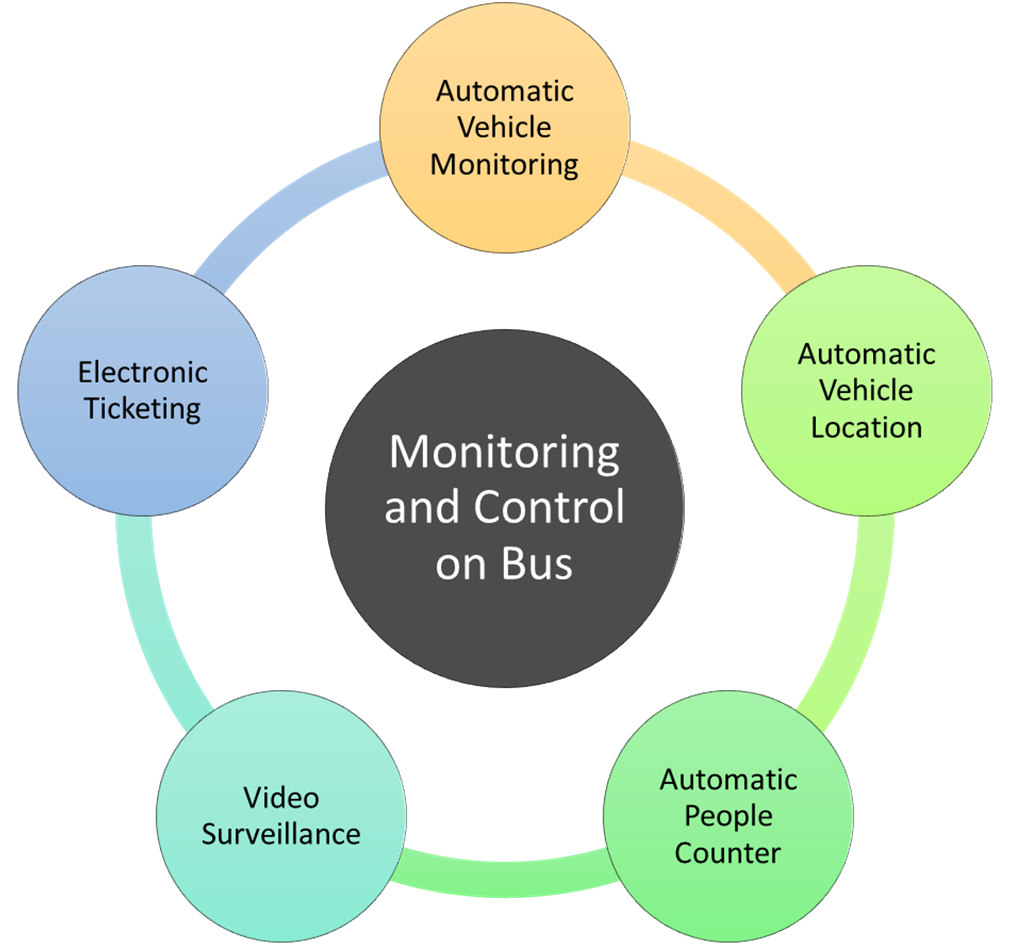
\includegraphics[width=0.4\textwidth]{Images/New Technologies/immagine intro Tech On.png}
    \caption{Technology Installed on Bus}
    \label{fig:onbus}
\end{figure}


The purpose of on – bus technology is mainly service monitoring and data gathering for demand analysis and offer adjustments, those type of system have become particularly relevant in the, very recent, Covid–19 period where it was particularly relevant analyze and report the mobility evolution to prospect near future scenarios and assess the effectiveness of adopted actions.


\paragraph{AVM and AVL}
Automated Vehicle Monitoring is a technology based on localization through GPS, monitoring and recording different topics related to moving vehicles, such as position, speed, diagnostic of mechanical components and so on. Automated Vehicle Location is more focused on the GPS position on the vehicle but if GPS signals are poor, AVL can use different technologies to determine actual location information, such as dead reckoning, which takes a previously determined position, and then incorporates estimations of speed, heading direction, and course over elapsed time. 

The buses, based on the GPS signal that the satellite sends, calculate their position a certain amount of seconds. This information, together with other data, is sent to the operator in the operation centre which operate in real-time the data and sends them to the costumer information management systems. Those data are also stored in order to make them available to the procuring entity for service reporting.

This type of technology allow the PTO to increase the security level and control in case of disruptive events, being able to handle and analyze big amount of data to assess a quick result or motivation.

Those technologies can be used to compute some interesting KPIs, tacking the status of the service, advances and delays, vehicle tracking, service adjustments in case of disruptive events. Also, from a graphical point of view the real-time situation can be displayed really well and it can be used widely in a dashboard.
\begin{figure}[H]
    \centering
    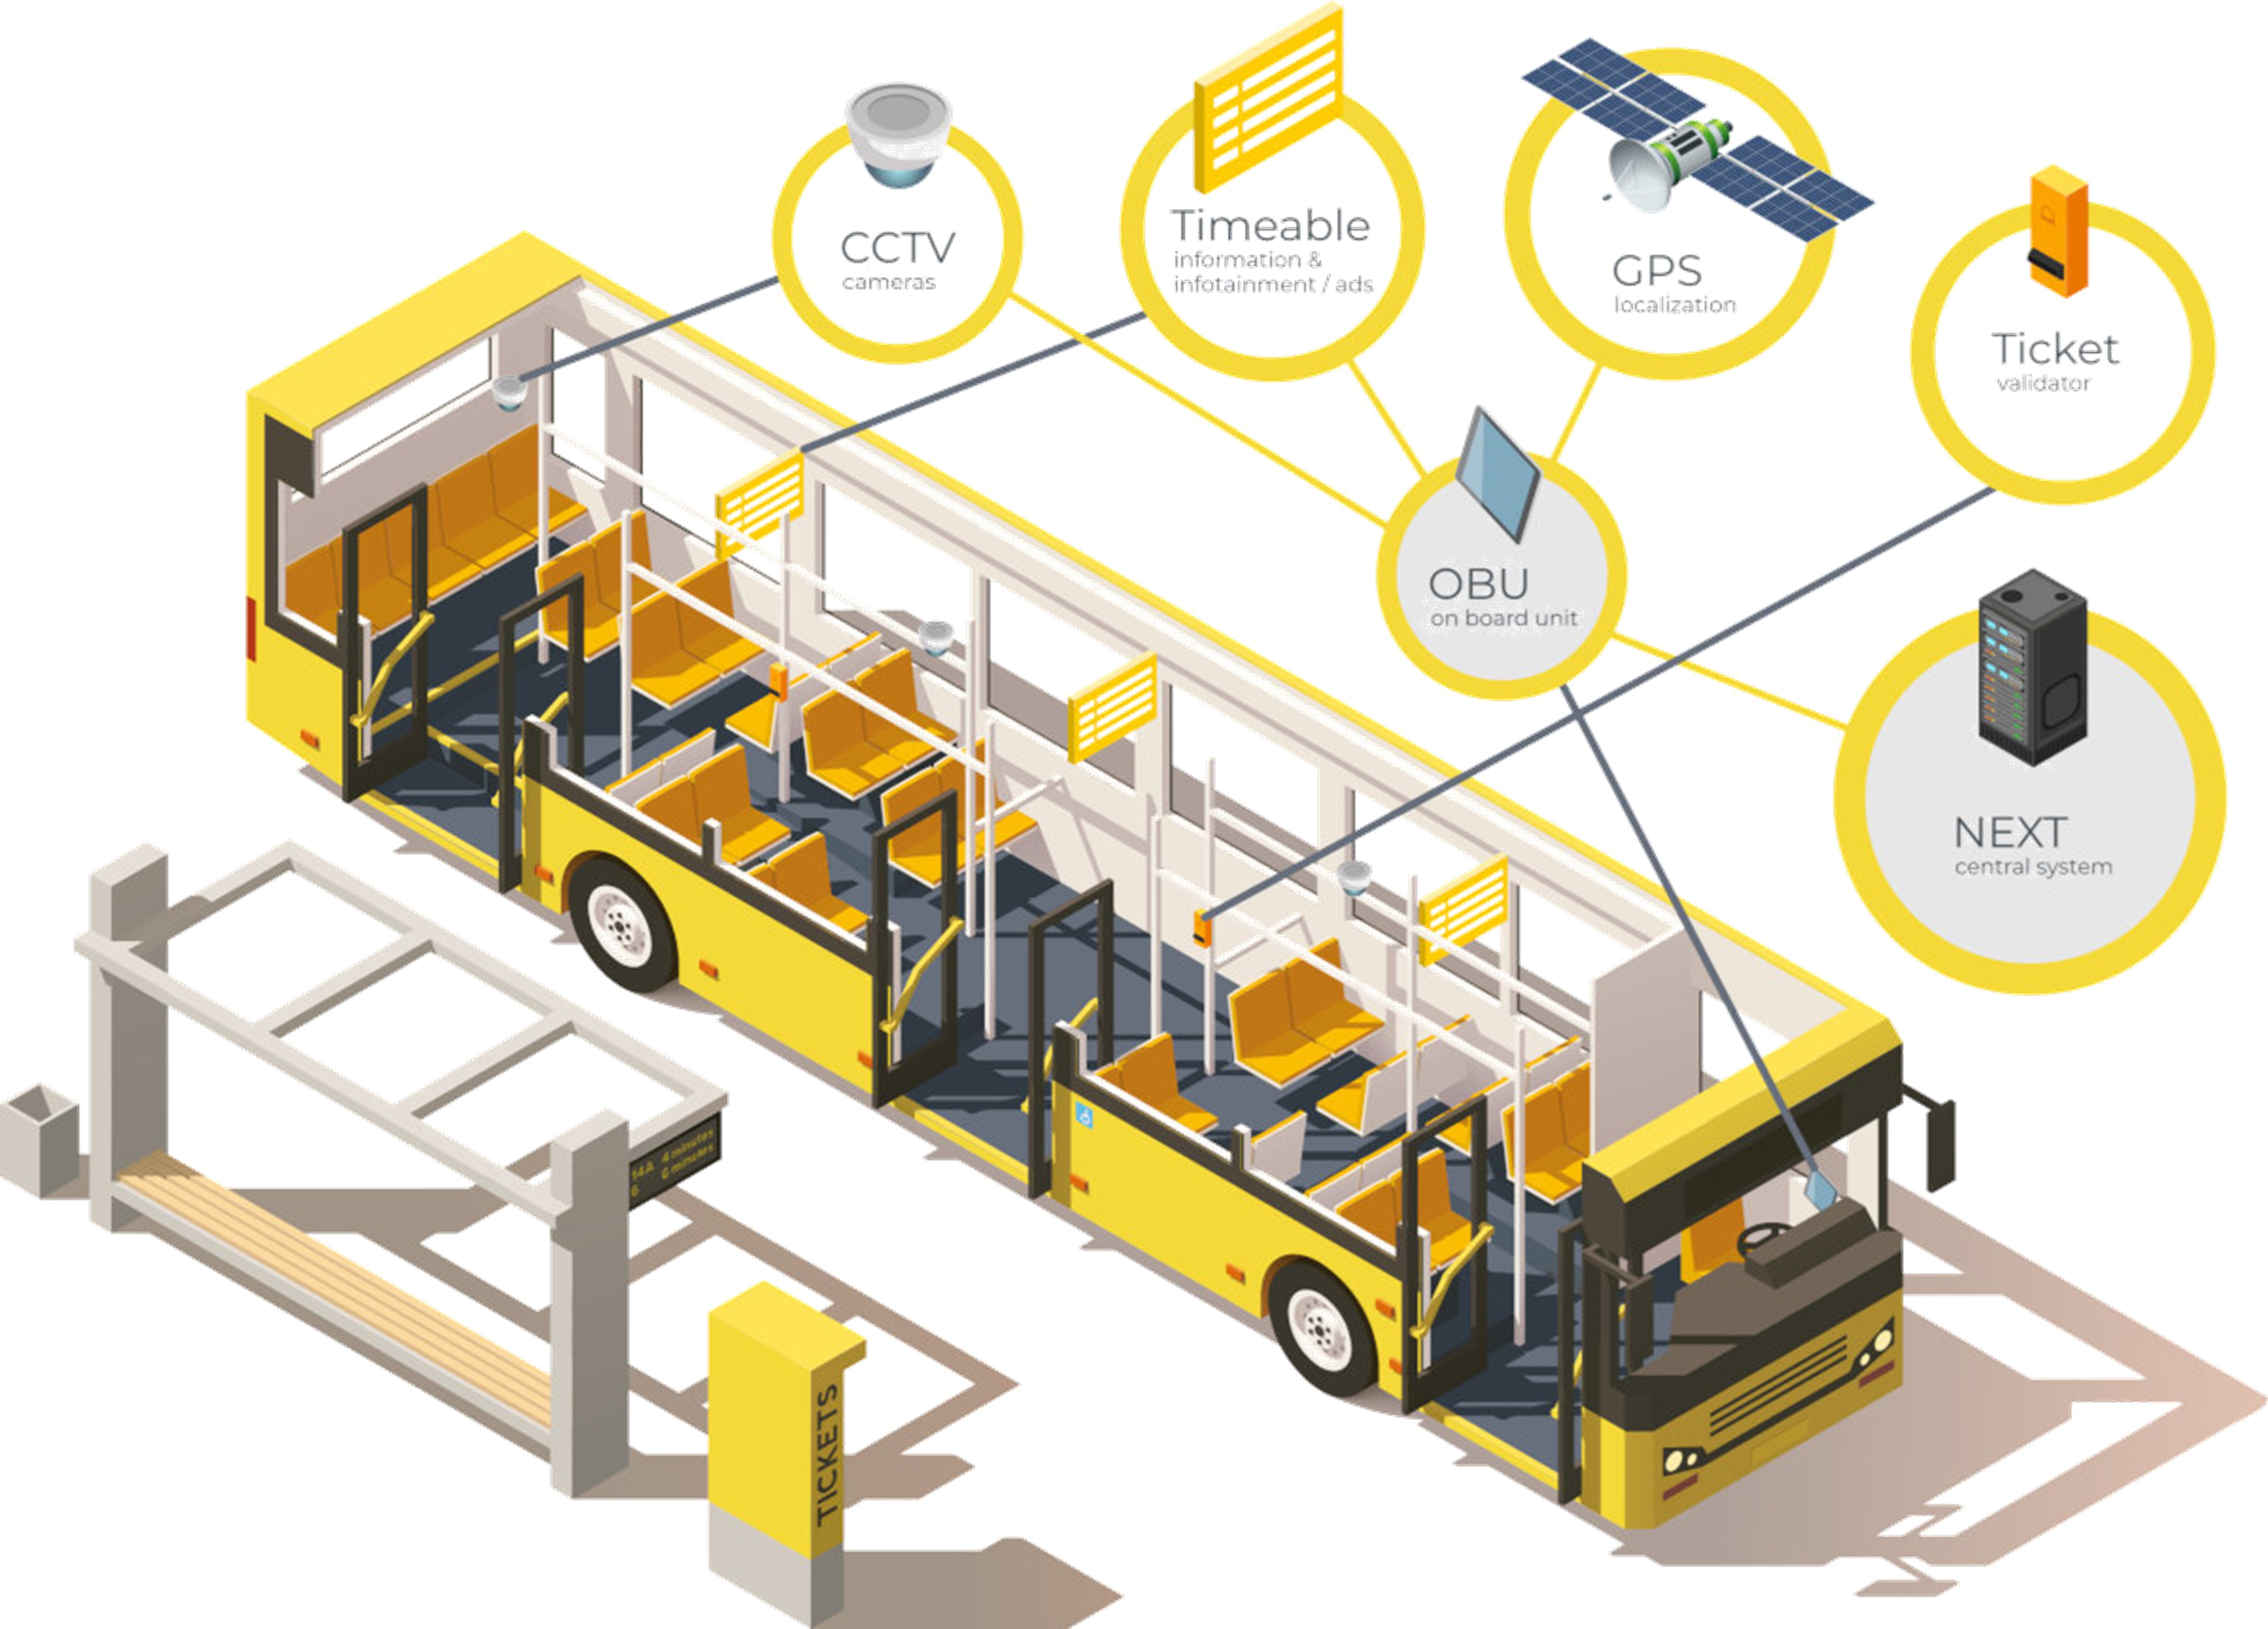
\includegraphics[width=0.7\textwidth]{Images/New Technologies/AVMeAVL.jpg}
    \caption{AVM and AVL\cite{avmavlimmage}}
    \label{fig:avmavl}
\end{figure}

\paragraph{Automatic People Counter}
People counters are electronic sensors that count people as they walk into an entrance. There are various methods for those systems to count people. Those can be classified into contact-type counters, sensors implemented system, and vision-based system using a camera. Contact-type counters are mechanical counters which need human contact such as turnstiles and mat-type foot switches that can obstruct the path. 

However, this type of counter only applicable for minimal people counting and it is not suitable for massive number of people, such as a high flow of people boarding or getting off the bus. Other technologies used in people counter are Pyroelectric Infrared (PIR) sensors, ultrasonic sound distance sensor and thermal sensor. PIR sensor counts people when they pass through the area of observation which is mounted with a pair of IR transceiver. Thermal sensors are only able to observe the crowd density without counting them accurately. 

\begin{figure}[h!]
    \centering
    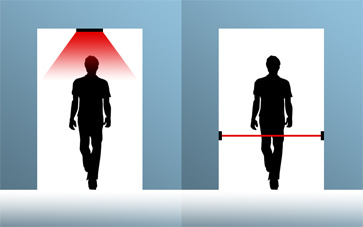
\includegraphics[width=0.5\textwidth]{Images/New Technologies/APC.jpg}
    \caption{Automatic People Counter\cite{apcimage}}
    \label{fig:APC}
\end{figure}

People counting technologies can be used for many purposes: assessing that is impossible to have them on all the lines of the consortium, it is possible to use a data analysis on routes that do not have APC to build a model to estimate the level of service onboard on all routes. The load factor information is very useful to consult on a real-time dashboard, creating a trend of the number of people on board; in this way it is also possible to study the performance of the stops, as well as the lines, creating a set of KPIs that can function both as real-time  indicators and for decision-making at a future planning level.

\paragraph{Video–surveillance }
Video-surveillance is a technology that is extremely helpful for public transport management; cameras can be installed in three main positions: outdoor cameras, to monitor the surrounding scene and in particular the blind spots, indoor cameras, to monitor bus passengers, and driver cameras, to monitor the driver behaviour. All those images can be provided to the driver with clear images referring to these areas, which can then be displayed on special monitors to be installed on the driver's dashboard. 

With the new telecommunication technologies, like 4G and 5G, it can be performed a sort of edge computing through the help of video analysis with AI systems; these methods can lead to fast and responsive actions or adjustment that the drivers, or the employees in remote, can do. Artificial Intelligence algorithms can detect some risk factors for what concern the ride’s safety, such as tiredness, distraction, or irregular behaviour of the driver.

\begin{figure}[h!]
    \centering
    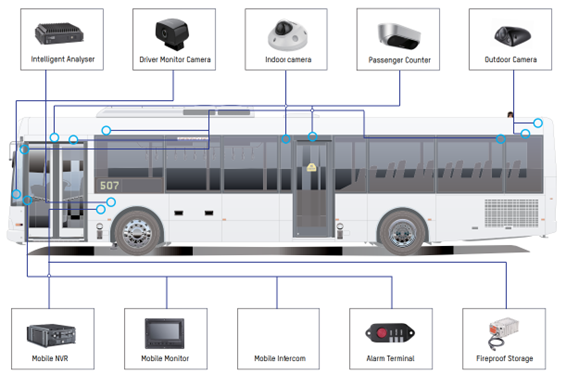
\includegraphics[width=0.6\textwidth]{Images/New Technologies/VIDEOSURV.PNG}
    \caption{Video–surveillance\cite{videosurvimage}}
    \label{fig:vs}
\end{figure}


\paragraph{Electronic ticketing systems}
The electronic ticketing system is not a proper technology installed just on buses, but the validation and control parts are managed largely on the bus. The system is composed by the validators and the On-Board Computer, which are installed directly on the buses, and by a central Control Center where all the data collection, management and distribution of incomes and emission or recharge of smart cards takes place.

\begin{figure}[h!]
    \centering
    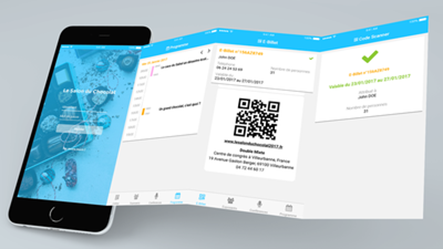
\includegraphics[width=0.45\textwidth]{Images/New Technologies/ELECTRONIC TICKET.png}
    \caption{Electronic ticketing systems\cite{eticketimage}}
    \label{fig:ets}
\end{figure}

One of the trending topics on the whole ticketing system is the type of support used: the support is the connection between costumers and PTO, which means that more information the support can bring to the PTO the better it is. In recent times there has been a rapid evolution of the support type, starting from basic paper, passing through magnetic, smart-cards and lastly mobile tickets. With Near-Field Communication (NFC) technology, the fares are redeemed without contact and completely remove the need to handle any physical cash or fares, and even limit the interaction needed with the driver. An additional motivation is that it is been found that physical money can carry the virus (in particular Covid-19) for up to three days, and by bypassing the need to purchase paper tickets and validate them, mobile ticketing can help reduce the transmission of the virus between riders and staff. An incredible by-product of integrating this technology is also the impact it has on the environment, as physical tickets no longer need to be created.

Keeping the user in mind, public transit technology is moving toward creating a more personalized ridership experience. A shift in this space is Account-Based Automatic Fare Collection. Through this system, all travel history, documents, and account information for riders is gathered in a customized dashboard.

With this technology, passengers can identify and participate with every available public service that is enabled for Account-based fare collection, making it far easier to use different modes of transportation, and save specific routes or journeys for use later. This also removes the hassle of having to manage multiple user accounts, payment methods, and receipt/billing information.

\subsection{Technologies installed off bus}
\label{subsec:techoffbus}
In addition to technologies directly installed on buses, there are some systems that play a center role in the world of public transport innovation, even not being directly on the public transport vehicle. Those type of technologies are aimed more at the network part of the service: we are talking about all the secondary, or subsidiary, technology that are vastly growing in the world, that together form the infamous Internet of Things. 

The general concept is that public transportation is affected by countless variables and not only by the ones directly connected to it, such as the costumers, the bus health, the drivers and so on, for example: the weather is clearly a source of data in correlation, but more importantly in causation, with the transportation system, if a day there is a particularly heavy rain, people tend to use more the private vehicle, using less the bus or in general the public transportation, this is due to the fact that often using PT means waiting outside under the rain. This situation have a great impact on the PTO systems, in fact bus tend to be less populated, so all the KPIs related to the number of costumers onboard are affected, as well as the travel time since, as said before, there are more private vehicles on the road than in a normal day; travel time therefore will be higher than usual and more delays, all of this affect the KPIs related to the commercial speed, travel time, delays per day and so on \dots

This big example is made to understand that the more data of different types are gathered daily, the more precise the analysis that a PTO can assess. In this new era of technology, especially now with the faster growing 5G, it is very important to take advantage of them, exploiting all of their potentialities.

The potential of digital applications and solutions for public transit is endless. Sensing devices and IoT technology are becoming more robust and low-cost, providing useful data for municipalities, fleet managers and even riders. For example, in Sweden a recent study used wireless sensors on city buses to monitor real-time air pollution. The sensors gave more accurate data on highly polluted urban areas, which led to better-informed city planning decisions and air quality improvement efforts. 

Telematics technology is also becoming a way to provide transportation fleet managers with real-time data to help identify and address things like temperature control, fuel levels, optimal driving routes, operating efficiencies and more. Predictive analytics allows for quick maintenance and better energy management, which is critical to addressing environmental impact.

Other important aspects on this topic are the actions that the PTA can take directly, for example, with the spread of smart cities, the necessary information and communication infrastructure lends itself well to intelligent traffic management systems. These systems allow centralised traffic control, enabling transit authorities to intelligently manage traffic lights, cameras, emergency routes and public transport routes.

Urban transit systems are also looking into how to incorporate rapid transit into existing systems. While this term most often refers to rapid transit trains or hyperloop systems, this can also refer to rapid transit buses, which have dedicated traffic lanes and priority at intersections; something that smart traffic management could help manage.


\subsection{New KPIs possibilities}
\label{subsec:newpossibilities}
As we have understood in the previous paragraphs, frequency in data–gathering is a key factor. Looking at the data provided to us is almost surprising that a company like Arriva, and all the consortium in general, has such a lack of detail in the available data. The dashboard built in the previous chapter has a potential, clearly limited by the frequency and the quality of what’s inside.

But why a higher frequency data – gathering is the base answer to most of the problems? Gathering more data more frequently means that it becomes much easier to understand trends, seasonalities, or particular micro – behavior that a monthly, or in some cases even yearly frequency cannot pick. In particular, algorithms like regression, classification, clustering, anomaly detection, and many others, work so much better with large quantities of data, and therefore understanding what they have to tell us is far easier.

Another strong motivation for why is essential to have data gathered more frequently is the possibility of expansion of the analysis that can be done: looking at a more detailed time span is useful to build a model on different types of time centered analysis, such as workdays vs. weekdays, peak hour vs. off-peak hours. The possibilities of Arriva, as now, are to compute KPIs based on the company trend of the month or year, which can hide an enormous quantity of information; having daily, hourly, or even more precise data, allows the analysts, and us, to build a dashboard with better KPIs.

\paragraph{Dynamic KPIs}
Other than more precise KPIs, gathering all those types of data can mean also being able to compute different \textit{types} of KPIs: we are used to looking at dashboards with basic cardinal numbers, which by definition are static and provide agglomerative information on the subject, such as a mean, a median, maximum or minimum and so on. 

Introducing the use of \textit{Dynamic KPIs} opens up a new dimension in the data – plane in which the analyst can look and assess more types of conclusions. The Dynamic KPI is a particular way to view a result where the user can look directly at the trend, in real-time of the data, but let’s make an example.

If we want to analyze the number of passengers onboard on a specific ride, until now the KPIs were all built as a mean number of the occupation onboard, representing the average number of passengers on that ride. But this information, which is still useful, don’t get us wrong, is not able to tell the users how the flow of passengers distributes among the stops of the ride. Using a dynamic KPIs that shows both the people loaded and unloaded at every stop, we can see in the data more information, such as a particular section in the run where there are very few people onboard, and if it is behavior repeated in time, this information is useful to assess some conclusion, such as remove some stops, add new ones and many more.

\begin{figure}[t]
    \centering
    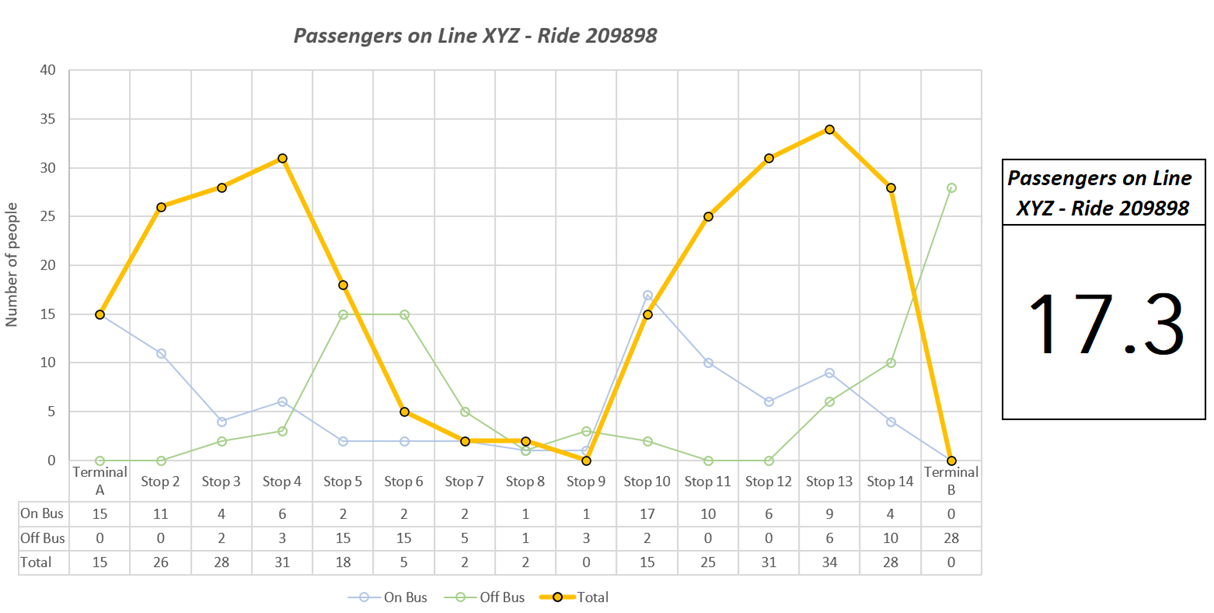
\includegraphics[width=1\textwidth]{Images/New Technologies/dynamic KPIs.png}
    \caption{Dynamic KPIs Example}
    \label{fig:dynKPI}
\end{figure}

As it is possible to see from the image  \ref{fig:dynKPI}, both are telling the same information, but in two different ways: the number on the right tells us just the mean number of passengers for that particular ride, although looking at the graph on the left we can detect much more information: the central stops of the ride (7, 8 and 9) are very little used, and also the number of passengers on board at that moment are almost zero. Here the PTO can make multiple decisions, such as dividing the line into two pieces to maximize the effectiveness of both of them. A deeper analysis can be done to understand why those stops are rarely used, maybe they can be re-positioned to meet higher demand, changing the line route by a little.




% Please add the following required packages to your document preamble:
% \usepackage{lscape}
%\newpage
\thispagestyle{empty}
%\begin{landscape}
\subsection{New Technologies KPIs examples}
\label{subsec:newKPIex}
Having know all the knowledge of new technologies that can be installed on and off the buses and all the new process that are involved to built more interesting KPIs, it is time to make some example, directly related to which data has Arriva now and what it could have in the future. In order to maintain the same scheme of pages in the traditional dashboard in \ref{ch:dashboard}, the KPIs are listed in the same structure:

\begin{table}[H]
\centering
\begin{tabular}{|l|l|l|l|}
\hline
\rowcolor{bluepoli!40}
\multicolumn{1}{|c|}{\textbf{KPI denomination}}                                       & \multicolumn{1}{c|}{\textbf{Technologies Used}} & \multicolumn{1}{c|}{\textbf{UoM}} & \multicolumn{1}{c|}{\textbf{Explanation}}                                                                                                                                                          \\ \hline
\begin{tabular}[c]{@{}l@{}}Daily single tickets   \\ sold over passenger \\ moved\end{tabular}  & Iot, E-Ticketing,   APC                & \begin{tabular}[c]{@{}l@{}} €\\ \ \# people \end{tabular}                                & \begin{tabular}[c]{@{}l@{}}Understand how\\ the amount \\ of single ticket sold affect \\ the overall passenger,\\  helping to size the service   \\ not only on historical \\ data and passes\end{tabular} \\ \hline
\begin{tabular}[c]{@{}l@{}}Distribution of   \\ ticket vs. pass per ride\end{tabular} & E-Ticketing, APC                     & \%                                            & \begin{tabular}[c]{@{}l@{}}Understand which   \\ type of costumer takes \\ certain rides allow to\\  assess decision for a ride\end{tabular}                                                       \\ \hline
\begin{tabular}[c]{@{}l@{}}Annual Fuel cost  \\  over km done\end{tabular}            & AVM, AVL                                        & €/km                                          & \begin{tabular}[c]{@{}l@{}}Helps understand the \\   driving behavior \\of the drivers \\ and the cost percentage \\ that affect \\the   balance sheets\end{tabular}                                   \\ \hline
\end{tabular}
\caption{List of new Economical and Financial KPIs}
\label{tab:economic}
\end{table}
%\end{landscape}
\newpage
% Please add the following required packages to your document preamble:
% \usepackage{lscape}
\newpage
\thispagestyle{empty}
\begin{landscape}
\begin{table}
\centering
\begin{tabular}{|l|l|l|l|}
\hline
\rowcolor{bluepoli!40}
\multicolumn{1}{|c|}{\textbf{KPI denomination}}                                                    & \multicolumn{1}{c|}{\textbf{\begin{tabular}[c]{@{}c@{}}Technologies \\ Used\end{tabular}}} & \multicolumn{1}{c|}{\textbf{\begin{tabular}[c]{@{}c@{}}Unit of\\  Measure\end{tabular}}} & \multicolumn{1}{c|}{\textbf{Explanation}}                                                                                                                                                        \\ \hline
\begin{tabular}[c]{@{}l@{}}Mean delay by time slot \\ (peak vs. off-peak) and ride\end{tabular}    & AVL, AVM                                                                                   & min                                                                                      & \begin{tabular}[c]{@{}l@{}}Understanding if a  \\delay is mainly caused \\ by the departing hour of the ride, \\ can help to modify   the schedule according to it\end{tabular}                    \\ \hline
\begin{tabular}[c]{@{}l@{}}Visualization on where \\ the ride generates the delay\end{tabular}     & AVL, AVM                                                                                   & map                                                                                      & \begin{tabular}[c]{@{}l@{}}Deepening the   knowledge of the delay \\ can mean even \\better improvements \\ going to make specific   changes \\ in some section of the lines\end{tabular}          \\ \hline
Lost costumers per   suppressed ride                                                               & APC, AVM                                                                                   & \#                                                                                       & \begin{tabular}[c]{@{}l@{}}Knowing how many   \\people are affected \\ by a suppressed ride\\ can help to assess \\ the importance of   that ride and an overall \\ level of discomfort\end{tabular} \\ \hline
Delay amount over mm   of rain                                                                     & AVM, IoT                                                                                   & min/mm                                                                                   & \begin{tabular}[c]{@{}l@{}}Knowing the relation  \\ between delays and \\ weather conditions\\ is important to correctly \\ dimension the   problem\end{tabular}                                     \\ \hline
\begin{tabular}[c]{@{}l@{}}Load Factor per run   \\ per time slot (peak vs. off-peak)\end{tabular} & APC, AVM                                                                                   & \%                                                                                       & \begin{tabular}[c]{@{}l@{}}Knowing the   percentage of load\\  for a particular run can help to allocate \\ better the resources\end{tabular}                                                    \\ \hline
Load Factor vs.   Weather Condition                                                                & APC, IoT                                                                                   & \%                                                                                       & \begin{tabular}[c]{@{}l@{}}Also in this case, knowing \\   the behavior in\\ different weather condition \\ can help to allocate better the resources\end{tabular}                                 \\ \hline
\end{tabular}
\caption{List of new Service Quality KPIs}
\label{tab:servicequality}
\end{table}
\end{landscape}
% Please add the following required packages to your document preamble:
% \usepackage[normalem]{ulem}
% \useunder{\uline}{\ul}{}
% \usepackage{lscape}
\newpage
\thispagestyle{empty}
\begin{landscape}
\begin{table}[]
\centering
\begin{tabular}{|l|l|l|l|}
\hline
\rowcolor{bluepoli!40}
\multicolumn{1}{|c|}{\textbf{KPI denomination}}                                                        & \multicolumn{1}{c|}{\textbf{Technologies Used}} & \multicolumn{1}{c|}{\textbf{Unit of Measure}} & \multicolumn{1}{c|}{\textbf{Explanation}}                                                                                                                                                                                                                             \\ \hline
\begin{tabular}[c]{@{}l@{}}Percentage of low environmental   \\ impact bus on the road\end{tabular}    & AVM                                             & \%                                            & \begin{tabular}[c]{@{}l@{}}Knowing how many green   bus \\ are circulating on the road can be \\ an interesting KPI to show at the PTA\end{tabular}                                                                                                                   \\ \hline
Percentage of km   made by hybrid/EV bus                                                               & AVM, AVL                                        & \%                                            & \begin{tabular}[c]{@{}l@{}}Same as before, knowing  how many kms \\ have been done in a healthy way is useful\end{tabular}                                                                                                                                            \\ \hline
Tons of $CO_2$ emitted   by bus or by line                                                             & AVM                                             & ton                                           & \begin{tabular}[c]{@{}l@{}}Understanding which   model of bus on which line\\  is the most emissive is useful to assess \\ how to renovate   the fleet\end{tabular}                                                                                                   \\ \hline
\begin{tabular}[c]{@{}l@{}}Tons of $CO_2$   \\ emitted in the city center vs. rural areas\end{tabular} & AVM, AVL                                        & ton                                           & \begin{tabular}[c]{@{}l@{}}Knowing the spatial   distribution of tonnage \\ emission can be useful to re-allocate different bus  \\  models on the lines\end{tabular}                                                                                                 \\ \hline
\begin{tabular}[c]{@{}l@{}}Mean bus consumption   \\ per run, per line, per bus type\end{tabular}      & AVL, AVM                                        & $L_{fuel}$/(run,   line, bus)                 & \begin{tabular}[c]{@{}l@{}}Awareness on bus   consumption by run is useful \\ to re-allocate and renovate the rolling stock\end{tabular}                                                                                                                              \\ \hline
Energy consumption curve   for EV bus                                                                  & AVM, AVL                                        & kWh/(time, km)                                & \begin{tabular}[c]{@{}l@{}}Having Electric Vehicle can be difficult to manage \\ in terms of recharging point and time allocation,  \\  understanding where the bus consume most \\ of its energy is handy to optimally   place \\ the recharging points\end{tabular} \\ \hline
\end{tabular}
\caption{List of new KPIs on Rolling Stock}
\label{tab:rollingstock}
\end{table}
\end{landscape}
% Please add the following required packages to your document preamble:
% \usepackage{lscape}
\newpage
\thispagestyle{empty}
% Please add the following required packages to your document preamble:
% \usepackage{lscape}
\begin{landscape}
\begin{table}[]
\centering
\begin{tabular}{|l|l|l|l|}
\hline
\rowcolor{bluepoli!40}
\multicolumn{1}{|c|}{\textbf{KPI denomination}}                                                       & \multicolumn{1}{c|}{\textbf{Technologies Used}} & \multicolumn{1}{c|}{\textbf{Unit of Measure}} & \multicolumn{1}{c|}{\textbf{Explanation}}                                                                                                                                                             \\ \hline
\begin{tabular}[c]{@{}l@{}}Commercial speed \\ deviation   from mean\end{tabular}                     & AVL, AVM, historical   data                     & $\pm$ km/h                                    & \begin{tabular}[c]{@{}l@{}}Comparing real-time   \\ commercial speed with the mean \\ of historical data help understand, \\ together   with delays information, \\ where is the problem\end{tabular} \\ \hline
Amount of km per day                                                                                  & AVM                                             & km                                            & Amount of kilometers   per day                                                                                                                                                                        \\ \hline
Planned vs. Effective   kms                                                                           & AVM                                             & \%                                            & \begin{tabular}[c]{@{}l@{}}Comparison between   \\ planned km on schedule \\ and km effectively done in a day\end{tabular}                                                                            \\ \hline
\begin{tabular}[c]{@{}l@{}}Mean time per stop   \\ (peak vs. off-peak)\end{tabular}                   & AVL                                             & sec                                           & \begin{tabular}[c]{@{}l@{}}Amount of time taken   at each stop to \\ loading and unloading the passengers\end{tabular}                                                                                \\ \hline
\begin{tabular}[c]{@{}l@{}}Stop time in   relation to number \\ of people moved per stop\end{tabular} & AVL, APC                                        & \# of people / sec                            & \begin{tabular}[c]{@{}l@{}}As the one above but    comparing it \\ to the number of people \\ that   actually moved\end{tabular}                                                                      \\ \hline
\begin{tabular}[c]{@{}l@{}}Commercial speed vs.\\ millimeters of rain/snow\end{tabular}               & AVL, IoT                                        & f(Km/h, mm)                                   & \begin{tabular}[c]{@{}l@{}}Comparison between mean  \\  commercial speed \\ of the ride and the amount \\ of rain fall in that period of   time\end{tabular}                                          \\ \hline
\begin{tabular}[c]{@{}l@{}}Commercial speed vs. \\ Fuel Consumption or $CO_2$ produced\end{tabular}   & AVL, AVM                                        & (km/h)/kWh, (km/h)/$tons_{CO\_2}$           & \begin{tabular}[c]{@{}l@{}}Helps understand the   driving behavior \\ of the drivers among with the points \\ where to optimize it\end{tabular}                                                       \\ \hline
\end{tabular}
\caption{List of new Operational KPIs}
\label{tab:operation_indication}
\end{table}
\end{landscape}

\subsection{Mock Up Dashboard}
The aim of this section is to built and visualize some mock-up dashboard pages, starting from the KPIs listed tables \ref{tab:economic}, \ref{tab:servicequality}, \ref{tab:rollingstock}, \ref{tab:operation_indication}.

We would like to point out that all pages are a mock-up also for what concerns the data present in he graphs, which may appear not close to the reality and made on purpose to talk about their benefits.

\newpage

\newpage
\begin{landscape}
\thispagestyle{empty}
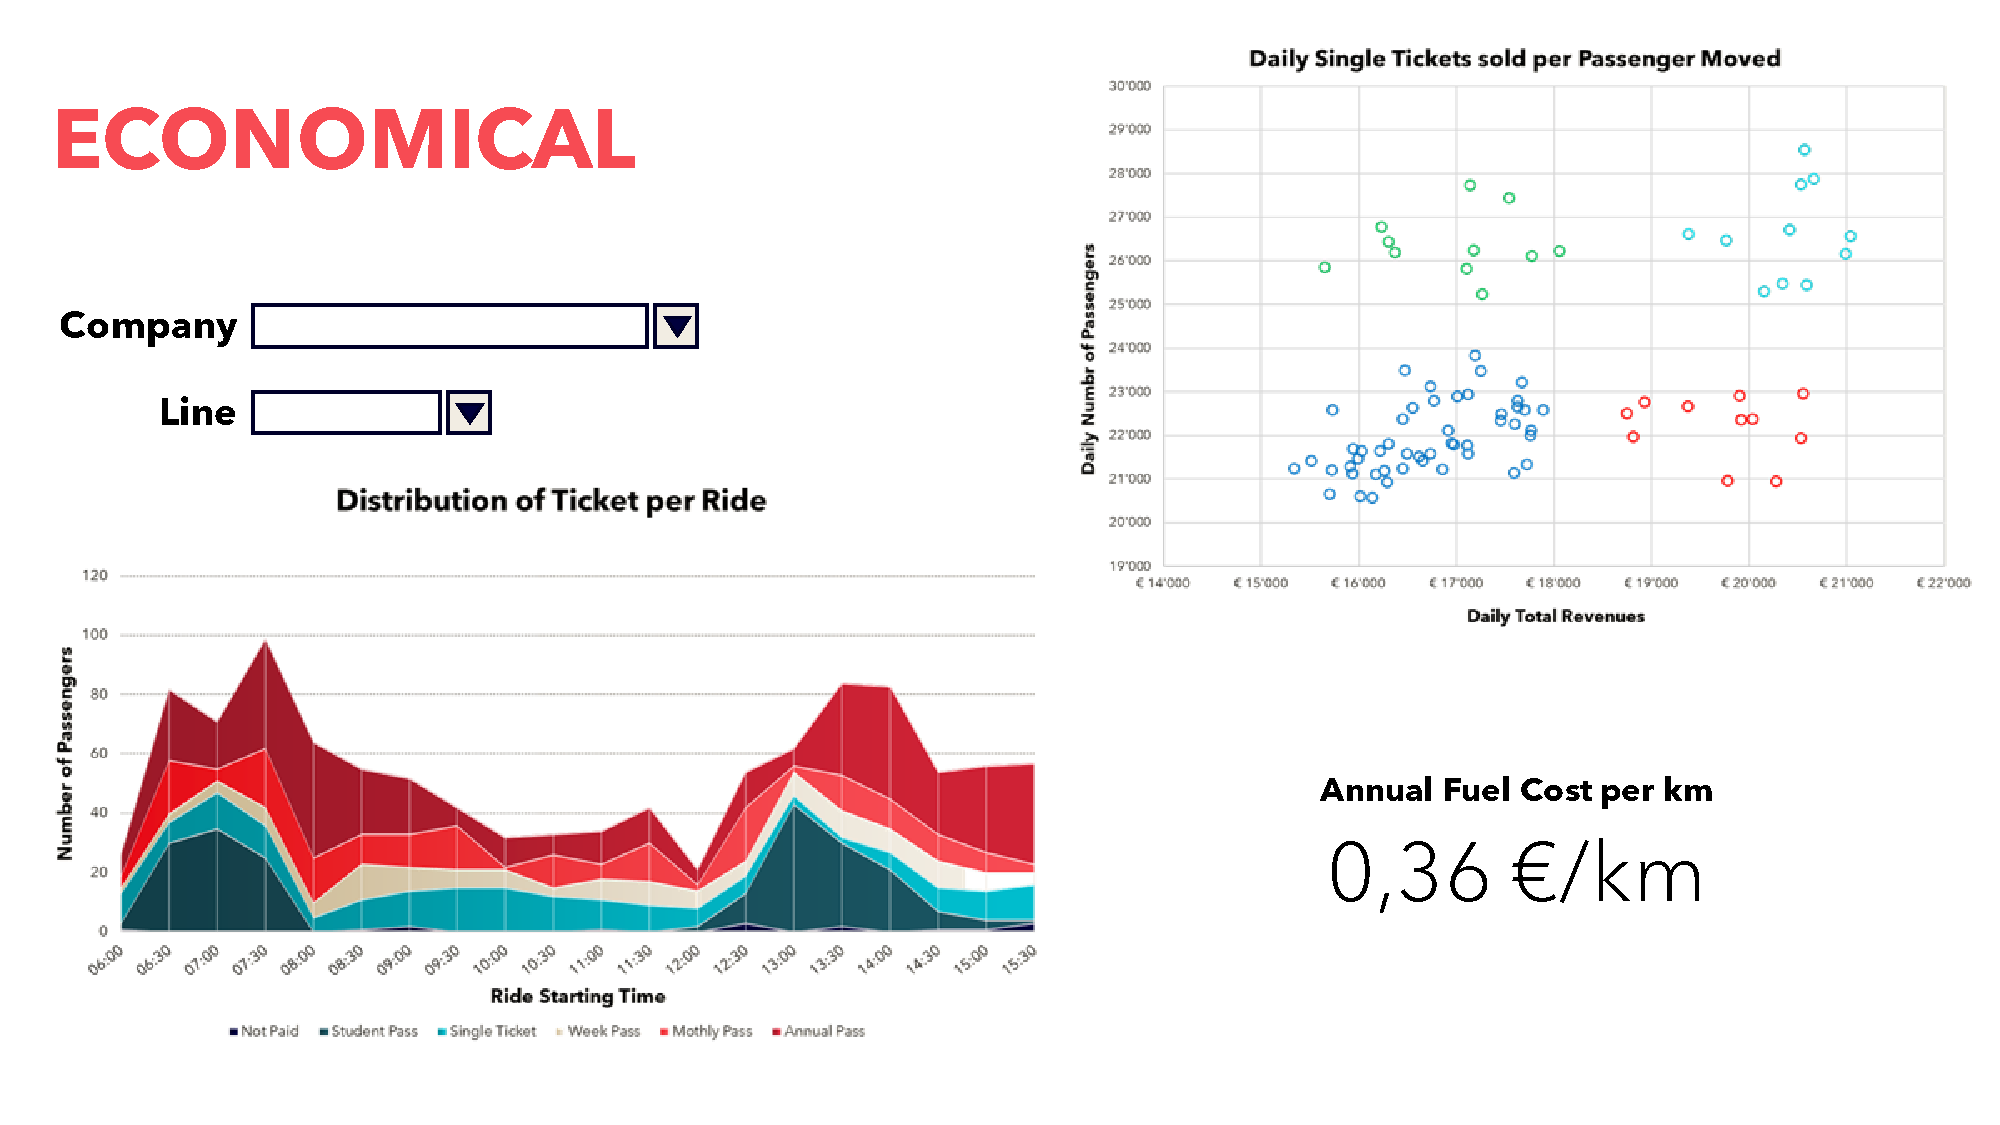
\includepdf[angle=90, pagecommand={\null\enlargethispage{3\baselineskip}\vfill\captionof{figure}{Economical page}\label{fig:ep}}]{mockup/economical.pdf}
\end{landscape}


\subsubsection{Economical page}
In this page we have created a visualization, in addition to the traditional one, able to tell a lot more information about the daily revenues of the company, for example, in the graph upright (\emph{Daily single tickets sold per passenger moved}) is possible to classify the dots (which each one represents a day) in four main areas:

\begin{itemize}
    \item \textcolor{blue}{\textbf{Blue Area}} is the normality, where average revenues are collected and the passengers moved are around a standard mean, depending, for example, from the day of the week of the time of the year.
    \item \textcolor{red}{\textbf{Red Area}} instead can represent the moment during the year where most people buy their monthly or yearly pass, which cause an abnormal amount of revenues, but still the passengers carried are quite constant.
    \item \textcolor{green}{\textbf{Green Area}} can be special day of the year, when maybe ticket office are closed (so less revenues from those), but a lot of people travel with public transport.
    \item \textcolor{cyan}{\textbf{Light Blue Area}} can represent some particular days when events happen, if Atalanta BC plays an important home game, a lot of supporters can choose to reach the stadium using public service, causing an substantial increase in the amount both in revenues and in passengers moved.
\end{itemize}

The graph in the lower-left part of the page shows the distribution of users of a particular line among its ride in the day. By visualizing how many people using different type of tickets have taken the bus, its possible to assess some actions regarding the advertising or the better sizing of the bus. So actions that can work on different levels: operational and marketing-wise.

\newpage
\begin{landscape}
\thispagestyle{empty}
\includepdf[angle=90, pagecommand={\null\enlargethispage{3\baselineskip}\vfill\captionof{figure}{Service Quality page}\label{fig:sqp}}]{mockup/service_quality.pdf}
\end{landscape}

\subsubsection{Service Quality page}
Understanding the quality of service is a key factor both for the operational and economical side of the company, but also for the costumer satisfaction. Assessing its behavior daily can be a big help in order to understand all the minor actions in which the company can work on.

This page mainly focus on the \emph{delay} and its variablily taking into account:
\begin{itemize}
    \item Time of the Day: Peak and Off Peak Hours
    \item Weather Conditions: millimeters of rain (or snow)
    \item Location of the delay accumulation
\end{itemize}

Those three information together can help to visualize how and where the rides \emph{accumulate the delay}: knowing if there is a relation between minutes lost and millimeters of rain can, for example, help to a better planning on a day to day basis. Instead, for example, knowing \emph{where is located} the delay accumulation is useful to assess some major changes on the line path or work together with the PTA to find a more powerful solution.

\newpage
\begin{landscape}
\thispagestyle{empty}
\includepdf[angle=90, pagecommand={\null\enlargethispage{3\baselineskip}\vfill\captionof{figure}{Rolling Stock and Operation page}\label{fig:sqp}}]{mockup/rolling_stock.pdf}
\end{landscape}

\subsubsection{Rolling Stock and Operation page}
This last page is more bus-centered, both looking at how the company is managing the fleet to be put on the road and assessing how well the fleet is performing looking at the Commercial Speed and the Energy Consumption curve.

The amount of green buses that a company have in their fleet is, and will be more and more, an important issue, we wanted to emphasize that by creating a visualization where is possible to know the percentage of Green Buses on road and with a visualization of the rolling stock composition.







\newpage
\section{Social Sustainability}
Social sustainability is a frequently disregarded part of sustainability, as supportable advancement discussions frequently centre around the natural or monetary parts of supportability. In fact, all three dimensions of sustainability must be addressed to attain the most sustainable outcome possible.

Social sustainability is a process for creating sustainable and successful places that promote well-being by understanding the needs of people in the places where they live and work. Social sustainability combines the design of the physical environment with the design of the social world: infrastructure to support social and cultural life, social services, systems for engaging citizens and spaces for people and places to evolve. 

A Public Transport company like Arriva is in constant contact with its customers, whose well-being is a key aspect of the company's success. it is therefore important to assess all the aspects of social sustainability, both on the customer side but also on the internal side of the company, concerning the employees.

Having said that, we will analyze three main aspects on this topic:

\begin{itemize}
    \item Workers’ Sustainability
    \item Quality of Service
    \item Cleanliness
\end{itemize}

\subsection{Workers’ Sustainability}
Employee sustainability is the current and future ability of workers to remain in the workforce and is determined by a healthy organizational culture that supports and values employees. A sustainable employee culture keeps employees engaged to the level needed to perform their jobs capably.

Organizations that are concerned with employee sustainability recognize the need to create environments where employees remain engaged, perform at a high level, and experience job satisfaction, job commitment, and cultural buy-in throughout the duration of their employment. 

As the workforce ages, more emphasis is being placed on the importance of sustainable employment, since workers of all age groups, including those just entering the workforce, are making employee sustainability a priority in their job search.

More and more job seekers are looking to join companies that are concerned not only with environmental sustainability but are dedicated to building a culture of employee sustainability within their organizations as well.

As introduced before in \ref{sec:Intro_Innvovative}, the Sustainable Development Goals are set reach many goals at humanity level, one of which is Social Sustainability; below are listed some of the SGDs that take into account specifically the workers’ sustainability.

\begin{figure}[h!]
    \centering
    \includegraphics[width=1\textwidth]{Images/Social_sustainability/SGD workers sustainability.PNG}
    \caption{SDGs related to Workers' Sustaibability}
    \label{fig:SDGworksus}
\end{figure}

\begin{description}
   \item[n°1 - No Poverty] According to the 1.3 SDG which aim at being able to defeat poverty, the salaries must be adjusted to the job position according to the national collective labour agreement. To monitor this aspect is useful to consider the following KPI:
   \begin{itemize}
       \item Average salary level in proportion to the national collective labour agreement
   \end{itemize}
   \item[n°4 - Quality Education ]The 4.4 SDG emphasises the importance of training education in workplace in order to have always better quality of service and to increase safety of workers and clients.
    \begin{itemize}
       \item Training hours per capita for traveling and non-traveling personnel
       \item \% Employees who received an evaluation during the year
   \end{itemize}
   \item[n°5 - Gender Equality ] In particular 5.5 SGD, prohibit any forms of discrimination and gender disparities in company employees (5.5 SDG). Some reference indicators to consider measuring the gender equity are the following:
   \begin{itemize}
       \item \% women in management area: more importance on the women full and effective participation and equal leadership opportunities at all levels of decision-making in political, economic and public life
       \item \% women with a permanent contract
       \item Ratio between training hour for woman and men
   \end{itemize}
   \item[n°8 - Decent Work and Economic Growth ] The 8 SDG remark the importance of an equal and fair salary for all workers, including young people and people with disabilities and the importance to reduce the percentage of unemployed young people who do not follow a course of study or who do not follow training courses. Going more in detail, the 8.2 SDG stresses the importance to achieve higher levels of economic productivity through diversification, technological updating and innovation, including through a focus on high value-added sectors and labour-intensive sectors. 
   \begin{itemize}
       \item \% employees with permanent contract
       \item \% employees under 35 
       \item \% turnover rate
       \item Frequency of injuries of workers
       \item Index of severity of injuries
       \item Number of hours of training on safety and health
       \item \% employees registered with trade unions
       \item Number of hours of trade union assemblies
       \item Complaints related to work practices
   \end{itemize}
   \item [n°9 - Industry, Innovation and Infrastructure ] The importance of accessing to information and communication technologies is remarked by the 9.6 SDG. In a transport company is essential to master this goal since it could provide a great amount of benefits in terms of real-time communication and feedback from the drivers on the road.
   \begin{itemize}
       \item \% Employees with company phone with application used by the company
   \end{itemize}
\end{description}

\subsection{Quality of Service}
For a long time, the performance evaluation of Public Transport (PT) has been carried out from the service managers’ perspective, based on the cost efficiency and cost effectiveness of PT services and operations. However, in the last few decades, Service Quality (SQ) has become a major area of attention for practitioners, managers and researchers, who have focused on the passengers' perspective.

The perception of Service Quality is the result of a comparison of consumer expectations with actual service performance perception or with ideal performance, depending on which type of approach we would look at. The existence of different methodologies could be justified by the complexity of the Service Quality concept, the number of attributes used to evaluate it, or the imprecision and subjectivity of the data used to analyse it, typically based on customer satisfaction surveys (CSS). 

We have considered two approaches at Service Quality in this report, one using the above cited SDGs that talk about this aspect and the other taking into account “Carta della Mobilità” of Arriva, produced every year, which is the document that regulates the relationship between PTO and the users.

\begin{figure}[h!]
    \centering
    \includegraphics[width=0.6\textwidth]{Images/Social_sustainability/SDG service quality.PNG}
    \caption{SDGs related to Quality of Service}
    \label{fig:SDGqualiserv}
\end{figure}

\begin{description}
   \item[n°3 - Good Health and Well-Being] The 3.6 SDG has the goal to halve the number of deaths and injuries from road traffic accidents worldwide by 2020. To monitor this aspect the following KPIs can be considered: 
   \begin{itemize}
       \item Number of injuries and deaths caused by road accidents
       \item Number of road accidents
   \end{itemize}
   \item[n°5 - Gender Equality]In SDG 5.1 the main focus is to end all type of discrimination, and for our purposes we have thought of some KPIs that can be useful to monitor for a PTO on this aspect: 
    \begin{itemize}
       \item \% female passengers: this information can be collected easily if the passenger register on the website or on the application of the company 
       \item Number of assaults and violence to women on buses
   \end{itemize}
   \item[n°16 - Peace, Justice and Strong Institution ]The has the goal by 2030, to reduce illicit financing and arms trafficking, enhance the recovery and return of stolen assets and fight all forms of organized crime, reduce corruption and all its forms (16.4), Develop effective, accountable and transparent institutions at all levels (16.6). 
   
   To monitor fare evasion, corruption and arms trafficking:
    \begin{itemize}
       \item Number of passengers checked
       \item Number of clients connected on social network
       \item Number of accesses to the site
       \item Courtesy of drivers, this information is already collected with the customer satisfaction survey
       \item Number of info point in the area 
       \item Number of point of sales of tickets in the area
   \end{itemize}
\end{description}

Then, as reported in the document \textit{Carta della Mobilità}, the quality of the service can be perceived through a series of fundamental factors that characterize the quality of each aspect of the trip (e.g. travel safety, regularity of the service, cleanliness and hygienic conditions of the vehicles, etc.) and, within each of these, by specific quality indicators (for example for travel safety: number of accidents, age of vehicles) which represent the performance levels of the service provided.

Each factor and quality indicator are associated with a value (which expresses the level of quality of the service actually provided) and a target set each year by the Company providing the service.
The data on customer satisfaction are collected, in accordance with the provisions of the service contracts, with surveys carried out every six months by an external market research company through response surveys. 

Going more in detail, the surveys analyse the following aspects with their respective KPIs:

\begin{itemize}
    \item {Safety of the trip}
\begin{itemize}
    \item Accidents of the vehicles
    \item Passive accidents
    \item Age of vehicles
    \item \textit{\textbf{Total perceived safety of the trip}}
\end{itemize}
    \item Personal and property safety
    \begin{itemize}
        \item	Complaints (theft and harassment)
        \item \textit{\textbf{Total perceived personal safety}}
    \end{itemize}
    \item Regularity and punctuality of the service
    \begin{itemize}
        \item Regularity of the service
        \item Frequency of rides
        \item Commercial speed
        \item Punctuality in rush hours
        \item Punctuality in non-rush hours
        \item \textit{\textbf{Total perceived regularity of the service}}
    \end{itemize}
    \item	Comfort and cleanliness of the buses
    \begin{itemize}
        \item Crowding in rush hours 
        \item Crowding in non-rush hours 
        \item Air conditioning
        \item Low-floor bus
        \item Additional services (mobile platform, wheelchair anchoring)
        \item \textit{\textbf{Total perceived comfort}}
        \item Ordinary cleaning
        \item Extraordinary cleaning
        \item Cleaning of bus stations
        \item \textit{\textbf{Total perceived cleanliness}}
    \end{itemize}
    \item Information and service to users
    \begin{itemize}
        \item Timeliness
        \item Internal visual devices
        \item Timetable at bus stops
        \item Point of sales of tickets
        \item Feedback to complaints
        \item \textit{\textbf{Total perceived information and services}}
    \end{itemize}
    \item Relational aspects
        \begin{itemize}
            \item  \textit{\textbf{Total perceived relational aspects}}
        \end{itemize}
    \item Attention to environment
        \begin{itemize}
            \item Electric or hybrid vehicles 
            \item Use of eco-fuels
            \item Vehicles Euro 3-4
            \item Vehicles Euro 4 and more
            \item \textit{\textbf{Total perceived attention to environment}}
        \end{itemize}
\end{itemize}

The KPIs are reported in the following graph, with a range value of [0,4]; as we can see, in 2019 there was an improvement in all indicators, except for the perceived security. For the year 2020 the data are not available because the surveys were not carried out due to the Covid pandemic.

\begin{figure}[h!]
    \centering
    \includegraphics[width=0.9\textwidth]{Images/Social_sustainability/graph.png}
    \caption{Summary KPIs related to "Carta della Mobilità" document}
    \label{fig:kpiscdm}
\end{figure}

\subsection{Cleanliness}
Since we are living in a very particular historic period where an excellent quality of sanitary conditions is essential, we wanted to deepen the aspect of Bus Cleanliness, already partially assessed in the chapter above.

Our interest was confirmed by the fact that cleaning requirements by the PTA has changed and become stricter. The importance of the cleaning is confirmed in the service contract, which establishes penalties in case of:
\begin{itemize}
    \item failure to comply the frequency and/ or cycles in relation to the individual types of intervention (both for ordinary and extraordinary cleaning of the fleet and infrastructure and network systems open to the public)
    \item Insufficient cleaning of the bus (both for ordinary and extraordinary cleaning of the fleet and infrastructure and network systems open to the public)
\end{itemize}

The main requirements for cleanliness in today's PTA are:

\begin{itemize}
    \item daily cleaning (ordinary cleaning): it consists of removing the filth produced by the passengers, cleaning of cockpit, floor and handrails (about 10-15 min per bus)
    \item monthly cleaning (extraordinary cleaning): it is a deeper cleaning; special products must be used to remove dirt (generally it takes at least 30-40 min per bus)
    \item half yearly cleaning: vehicles are subjected to an antibacterial sanitization and disinfestation cycle 
\end{itemize}

Nowadays, due to the pandemic situation, the consortium has introduced from March 2020 sanitation interventions with disinfection and sanitization in particular of the surfaces and passenger support points. Also, every fifteen days during the periodic cleaning interventions are performed cleaning by ionization

\subsection{Mock Up Dashboard}
As per the previous chapter \ref{sec:newtech}, the aim of this is to built and visualize some mock-up dashboard pages, starting from the KPIs listed above in the previous paragraphs.

Also for this section, all pages are a mock-up also for what concerns the data present in he graphs, which may appear not close to the reality and made on purpose to talk about their benefits.

\newpage

\newpage
\begin{landscape}
\thispagestyle{empty}
\includepdf[angle=90, pagecommand={\null\enlargethispage{3\baselineskip}\vfill\captionof{figure}{Workers' Sustainability page}\label{fig:work2}}]{mockup/workers.pdf}
\end{landscape}

\subsubsection{Workers' Sustainability}
The dashboard shows the main features of workers sustainability. All the data necessary to build this type of dashboard are already available within the company and do not risk additional technologies.In order to guarantee equal treatment between men and women also in the workplace, it is also necessary to know the proportion of men and women both in the managerial area and among the traveling staff.
another indicator to monitor inequalities is the type of contract offered to men and women (permanent contract, internship, part-time contract).
Safety is also essential in the workplace. to safeguard workers' lives, in addition to strict controls on safety provisions, it is also necessary to inform and train staff. For this reason, the dashboard shows the number of hours of training followed on average by each worker. For the various indicators a trend is reported from 2018 to 2021 in order to see the improvements, as in this case, or to be able to find the critical issues and solve them.

\newpage
\begin{landscape}
\thispagestyle{empty}
\includepdf[angle=90, pagecommand={\null\enlargethispage{3\baselineskip}\vfill\captionof{figure}{Quality of Service page}\label{fig:qs}}]{mockup/qualitysocial.pdf}
\end{landscape}

\subsubsection{Quality of Service}
The data regarding the quality of the service are collected through an annual questionnaire and are therefore already available. the dashboard in particular shows the parameter concerning the comfort and cleanliness at the edge of the vehicles. it is important to note how this parameter has changed over the years and also to break down this parameter to see what are the aspects on which it is possible to improve. furthermore, through the new technologies presented above, such as the people counter, a more objective value can be given to the parameter concerning the crowding of vehicles.

At the bottom of the dashboard some data are provided regarding the number of people registered on the company's social channels and the number of applications or accesses to the official website. these aspects of the service, considered in the past less important, are useful because they are closely related to both customer loyalty and fare evasion





\newpage
\section{Green Sustainability}
\label{sec:greensus}
The management of environmental aspects in a public transport company is aimed at their continuous improvement in terms of elimination, reduction or improvement of performance.

For uniform, transparent, goal-oriented and regulation-compliant management, we have to use of a set of procedures built from initial environmental analyses. The main environmental aspects that can be identified among all the material issues are:
\begin{itemize}
    \item Emissions into the atmosphere
    \item Energy Utilization
    \item Water Waste
    \item Waste Production
    \item Use of raw materials and natural resources
    \item Soil Contamination
    \item Dust, odors, vibrations, noise and visual impact problems
\end{itemize}

The significance of impacts can be assessed according to typical environmental analysis criteria, related to the severity, size and frequency of events, taking into account their controllability, applicable legal requirements and the expectations of stakeholders - local communities, employees and public administration. 
The Sustainable Development Goals \ref{ch:Innovative} considered under this aspect are mainly five:
\begin{itemize}
    \item \textbf{n°6 – Clean Water and Sanitation}, for what concerns water waste and overall consumption
    \item \textbf{n°7 – Affordable and Clean Energy}, in particular, considering all the types of energy consumption that a public transport service company have
     \item \textbf{n°11 – Sustainable Cities and Communities}, in particular the 11.6, concerning the emission environmental impact on cities
    \item \textbf{n°12 – Responsible Consumption and Production}, for what concerns raw materials consumption and waste management
    \item \textbf{n°13 – Climate Action}, to combat climate change taking into account all the aspects related to rolling stock, atmospheric and greenhouse emissions
\end{itemize}

\begin{figure}[!ht]
    \centering
    \includegraphics[width=1\textwidth]{Images/Green Sustainability/SDGs green.png}
    \caption{Green Sustainability SDGs}
    \label{fig:grsussdg}
\end{figure}

Regarding the five areas of interest in the SDGs \ref{fig:grsussdg}, it can be built a set of KPIs according to the goals previously stated.
We have decided to analyze three big groups of aspects related to the green sustainability:

\begin{itemize}
    \item \textbf{Energy Consumption} will focus on the amount of energy consumed and how it is distributed among all the activities that a PTO has to undertake. The aim is to reduce the consumption in the most efficient way.
    \item \textbf{Emissions} is one of the major topics related to Green Mobility and it is clearly essential to assess its problem and some way to keep track of it.
    \item \textbf{Waste} will be the last aspects taken into account, where we will focus on how to optimize both residual waste and water discharges.
\end{itemize}

\subsection{Energy Consumption}
\label{subsec:enecons}
Referring at the SDG number 7 \ref{par:onuobjectives}, by 2030 companies have to significantly increase the share of renewable in the global energy mix and double the global rate of energy efficiency improvement.
Energy consumption is mostly derived from bus fuels, which can be reduced through fleet renewal, maintenance activities and improved driving style. In addition to the consumption of buses, other sources of consumption have to be monitored, such as the electricity, natural gas and heating oil at the operational sites.
Looking at the overall activities that a company can perform, here in the table \ref{tab:sourceconsumption} are listed some of the main sources of consumption:

\begin{table}[!ht]
\centering
\begin{tabular}{l|l|}
\cline{2-2}
                                            & \cellcolor{bluepoli!40}Consumption   of:                                                                                 \\ \hline
\multicolumn{1}{|l|}{Running Buses}         & \begin{tabular}[c]{@{}l@{}}Fuel (diesel and natural gas)\\ Urea (Ad Blue)\\ Antifreeze\\ Lubricants\\ Tyres\end{tabular} \\ \hline
\multicolumn{1}{|l|}{Bus Maintenance}       & \begin{tabular}[c]{@{}l@{}}Spare parts\\ Electrical energy\end{tabular}                                                  \\ \hline
\multicolumn{1}{|l|}{Vehicle Cleaning}      & \begin{tabular}[c]{@{}l@{}}Water resources\\ Electrical energy\\ Detergent consumption\end{tabular}                      \\ \hline
\multicolumn{1}{|l|}{Refuelling}            & Electrical energy                                                                                                        \\ \hline
\multicolumn{1}{|l|}{Vehicle Storage}       & \begin{tabular}[c]{@{}l@{}}Soil\\ Electrical energy\end{tabular}                                                         \\ \hline
\multicolumn{1}{|l|}{Administration}        & \begin{tabular}[c]{@{}l@{}}Methane\\ Soil   \\ Electrical energy\\ Office supplies\end{tabular}                          \\ \hline
\multicolumn{1}{|l|}{\begin{tabular}[c]{@{}l@{}}Supply of goods, \\ materials and services\end{tabular}} & Fuel, Electrical energy, Office supplies                                                               \\ \hline
\end{tabular}
\caption{Main Sources of Consumption for a LPT company}
\label{tab:sourceconsumption}
\end{table}

With that in mind we can identify a set of indicators that can help monitor all of those aspects:
\begin{itemize}
    \item Gasoline and Methane consumption in GJ per km traveled by year
    \item Electrical Energy share usage with respect to previous years
    \item Green Energy used in each activity share
    \item Electricity Consumption share for electricity and heating of offices and sites compared to total energy consumption
    \item Green or Renewable fuel share over the totality of fuel used
    \item Energy Consumption share in relation to every km traveled with respect to the previous year
\end{itemize}

\subsection{Atmosphere and GHG Emissions}
\label{subsec:ghgemissions}
Between 1990 and 2018, emissions of all greenhouse gases in Italy decreased from 516 to 428 million tonnes of CO2 equivalent, a change achieved mainly by reducing carbon dioxide emissions, which contribute 81.4 \% of the total. Emissions in 2015 were 17.1\% lower than in 1990.

\begin{figure}[!ht]
    \centering
    \includegraphics[width=1\textwidth]{Images/Green Sustainability/GHG emission.png}
    \caption{Greenhouse gas emissions from transport in the EU, by transport mode and scenario \cite{GreenhouseScenario}}
    \label{fig:ghgemissions}
\end{figure}

The energy production and transport sectors are the most important, contributing half of the national climate gas emissions. Compared to 1990, however, GHG emissions from the transport sector show a slight increase (3.2\%), while emissions from energy production and industrial installations are clearly decreasing (-23.7\% and -38.9\% respectively).

In this scenario, sustainable mobility is destined to play an important role since the increase in Local Public Transport can make a significant contribution to reducing emissions: Arriva therefore has to contribute to the transition to more energy and emission-efficient transport.
There are some actions that the company can undertake in order to commit gradually to this cause, such as:
\begin{itemize}
    \item Identify the activities that produce direct and indirect emissions both at atmospheric level and at greenhouse level
    \item Monitor and analysis of the emissions produced
    \item Implement projects and actions aimed at reducing them as well as measuring their effectiveness
    \item Raise internal and external awareness of this issue through reporting and communication to the stakeholders.
\end{itemize}

Greenhouse gas emissions can be reported in accordance with the GHG protocol (Greenhouse Gas protocol) \cite{ghgprotocol} which provides for the distinction into three categories:
\begin{description}
   \item[Scope 1] Direct emissions from the combustion of fossil fuels (diesel and natural gas) for road transport - bus fleet and car fleet - for the production of thermal energy and emissions of refrigerant gases from air conditioning systems. 
   \item[Scope 2] Emissions resulting from the production of electricity taken from the grid and consumed for the operation of plants and for lighting; the company is indirectly responsible for the emissions generated by the energy supplier for the production of the energy required. 
   \item[Scope 3] Indirect emissions, other than those from electricity consumption, which are a consequence of the company's activities and which arise from sources not owned or controlled by other organizations. The boundary of Scope 3 is defined by the organization and generally includes what can be quantified and influenced by the company.
\end{description}

As a partial solution for direct atmosphere emissions from the rolling stock, vehicles can be equipped with the innovative SCR - Selective Catalytic Reduction - system, which uses urea-based liquid, to reduce exhaust emissions in terms of particulate matter and nitrogen oxides. The system is able to reduce harmful substances in the exhaust gas of diesel vehicles by up to 80 per cent.

Wanting to quantify all of that, here below are listed some example KPIs:
\begin{itemize}
    \item Emissions of greenhouse gases (CO2, CFCs, CH4, etc.) per passenger transported or per km travelled
    \item Generic emissions (PM, VOCs, NOx, CO, etc.) per passenger transported or per km travelled
    \item Air quality standards and management plans. 
    \item Rolling Stock share with Euro5, Euro6 or EEV motorization
    \item Total km travelled by low-impact buses share
\end{itemize}

\subsection{Water Discharges and Waste Management}
\label{subsec:water}
The production of waste mainly originates from maintenance activities and bus washing. Improve the quality of water discharges from washing vehicles that may contain pollutants, such as hydrocarbons, oils and various powders is a main component of the green approach of a company Along with adequate purification plants regular inspections of the plants should be carried out, directly by the company. In the event of an emergency situation, all activities that produce water to be purified destined for the plant concerned should be suspended until the plant is operational again.

Purifiers and absorbent material will produce sludge, extracted during inspections and maintenance, which have to be stored in the plants themselves or in labeled containers at each site. The frequency of interventions has to be established on the basis of the indications in the maintenance booklets and those provided by the installer, as well as the actual use of the systems.

Storm water runoff from forecourt areas should be conveyed to plants for treatment, as required by regulations. To avoid possible contamination of runoff water the PTO can take some precautionary measures, such as:
\begin{itemize}
    \item Workshop activities have to take place in covered areas without sumps
    \item Waste storage have to takes place in covered areas and containers
    \item Storage areas that could give rise to environmental impacts on water discharges must be included in a water discharge monitoring plan
    \item Sumps and collection tanks must be inspected periodically and cleaned at least once a year
 \end{itemize}

According to all the procedures listed above, we have selected a list of KPIs that could be useful to track down this particular topic inside the company:

\begin{itemize}
    \item Liters shares of reused water
    \item Liters of storm water saved per year
    \item Tons of waste generated per year
    \item Mean time to inspection on service hours
    \item Percentage of hazardous waste recovered
    \item Tons of waste produced per 1000km traveled
\end{itemize}

\subsection{Mock Up Dashboard}
As per the previous chapter \ref{sec:newtech}, the aim of this is to built and visualize some mock-up dashboard pages, starting from the KPIs listed above in the previous paragraphs.

Also for this section, all pages are a mock-up also for what concerns the data present in he graphs, which may appear not close to the reality and made on purpose to talk about their benefits.

\newpage

\newpage
\begin{landscape}
\thispagestyle{empty}
\includepdf[angle=90, pagecommand={\null\enlargethispage{3\baselineskip}\vfill\captionof{figure}{Green Sustainability page}\label{fig:work}}]{mockup/green.pdf}
\end{landscape}

\subsubsection{Green Sustainability}
This page mainly helps the observer to look at the development of green indicators by comparing values from year to year. A much more specific set-up could also be devised, to, for example, follow the trend of emissions, energy consumed, etc., on a daily or weekly basis during the year; in this case it would also be possible to activate preventive measures in case the values are too high compared to average trends or new limits imposed by regulation.
Having a clear view of how emissions and the quantity of environmentally friendly vehicles are being managed guarantees a strategic advantage at the planning level.

In addition, data on emissions or consumption can also be useful with a much higher frequency of collection, so as to be prepared in case the PTA requires immediate changes, such as a restriction on the circulation of certain types of vehicles for a few days to reduce smog in residential areas.
 

\addtocontents{toc}{\vspace{2em}}
\newpage
\section{Maintenance \& Fleet Management}
Maintenance is a key factor in a Public Transport Service company, in particular the aim is to optimize maintenance both for what concern the active maintenance time, but also  for what concerns the reliability of all the rolling stock components.

The traditional KPIs that can generally help to assess the impact of the maintenance in a PTO can be:

\begin{description}
    \item [Unscheduled or scheduled downtime] it helps maintenance managers to analyze how successfully they have implemented maintenance strategies:
        \begin{equation}
            D (\%)= \frac{hour\:of\: unscheduled\:or\:scheduled\:downtime}{total\:time\:period}\cdot 100
        \end{equation}
        And related to that, the downtime affects the cost as:
        \begin{equation}
        D_{cost} (\$/h)= unit\: per\: hour\: \cdot\: profit\: per\: hour
        \end{equation}
    \item [Mean Time Between Failures (MTBF)]
        \begin{equation}
            MTBF = \frac{operating\:time\:hours}{number\:of\:failures}
        \end{equation}
    \item [Mean Time To Repair (MTTR)]
        \begin{equation}
            MTTR = \frac{total\:maintenance\:time}{number\:of\:repairs}
        \end{equation}
    \item [Ratio of Budgeted vs Actual Maintenance Costs] It's possible to categorize the costs into unplanned and planned maintenance, in order to find areas for improvement:
        \begin{equation}
            budgeted\:vs\:actual\:maintenance\:costs = \frac{actual\:maintenance\:cost}{budget}
        \end{equation}    
\end{description}


\subsection{Electric Bus and Infrastructure}
\label{sec:elbusinfra}
Electric buses and generally electric vehicles need their own charging infrastructure depending on their battery’s specification which is highly expensive itself. Building infrastructure for electric buses requires high financing resources and subsidiaries from PTA except if PTO wins a long-term concession. By assuming that PTO undertakes a long-term concession, the most relevant and non-negligible KPIs are gathered.

Here below we mentioned some generic important KPIs, which affect the public, end-users, and PTO commonly, in case of cost, energy, and maintenance related to the bus and its infrastructure including charging in depot and opportunity charging.

\begin{description}
    \item [Total Cost of Infrastructure] which can be divided in the following costs:
        \begin{itemize}
            \item Electric Vehicle + Battery
            \item Opportunity Charging System
            \item Charging point + Charging pole + Installation cost + Smart Charging + ICT Compliance (for charging in depot)
            \item Energy Cost
            \item Electricity Network Losses
            \item Scheduled and unscheduled repair cost of bus, battery, charger and infrastructure
        \end{itemize}
    \item [Energy Consumption] The Energy demand (KWh) can be computed as the the sum of Energy demand for single charging by opportunity charging and the Energy demand for single charging by charging overnight in depot
    
    The Energy consumption of HVAC (KWh) is instead equal to the Energy consumption due to Heating, Ventilation and Air Conditioning system
    \item [Maintenance] The total maintenance time (hours) is equal to the duration of unscheduled and scheduled repair of bus, battery, charger and infrastructure
    
    Total MTBF is the number of failure per operational hours of bus, battery and infrastructure
\end{description}


\subsection{Hydrogen bus and Infrastructure}
As mentioned in \ref{sec:elbusinfra}, it is assumed that PTO wins a long-term concession in which the chance of building the infrastructure gets higher. The most relevant KPIs related to both infrastructure and fuel cell bus were collected.

\begin{figure}[h!]
    \centering
    \includegraphics[width=0.6\textwidth]{Images/manteinance/areas_hydrogen.png}
    \caption{Areas covered in hydrogen refueling infrastructure performance assessment }
    \label{fig:areashydrogen}
\end{figure}

In terms of the performance assessment, the hydrogen refueling infrastructure consists of four areas: 

\begin{itemize}
    \item On-site hydrogen production in the HPU (Hydrogen Production Unit)
    \item Hydrogen compression, storage, and dispensing in the HRU (Hydrogen Refueling Unit)
    \item External hydrogen delivery
    \item Aspects related to the operation of the entire HRS (Hydrogen Refueling Station). 
\end{itemize}

The indicators for assessing the performance of the hydrogen refueling infrastructure and its major elements can be found in the following set of tables: 
\begin{itemize}
    \item On-site hydrogen production in the HPU (Table \ref{tab:hpu})
    \item Hydrogen compression, storage, and dispensing in the HRU (Table \ref{tab:hru})
    \item Aspects related to the operation of the entire HRS (Table \ref{tab:hrs})
\end{itemize}

% Please add the following required packages to your document preamble:
% \usepackage{multirow}
% \usepackage{graphicx}
\begin{table}[p]
\centering
\resizebox{\textwidth}{!}{%
\begin{tabular}{|l|l|l|}
\hline
\rowcolor{bluepoli!40}
\multicolumn{1}{|c|}{\textbf{KPI Name}} &
  \multicolumn{1}{c|}{\textbf{period}} &
  \multicolumn{1}{c|}{\textbf{Unit of measure}} \\ \hline
Availability of the HPU &
  \multirow{3}{*}{Monthly, annually and overall} &
  \% \\ \cline{1-1} \cline{3-3} 
\begin{tabular}[c]{@{}l@{}}Amount of hydrogen produced \\ by the HPU and \\ by eachof its electrolysers/reformers\end{tabular}  &  & \%     \\ \cline{1-1} \cline{3-3} 
\begin{tabular}[c]{@{}l@{}}Specific water consumption \\ for hydrogen production\end{tabular} &
   &
  liters/Nm3 or liters/kg \\ \hline
HPU downtime &
  \multirow{2}{*}{Annually and overall} &
  hours \\ \cline{1-1} \cline{3-3} 
\begin{tabular}[c]{@{}l@{}}Specific energy consumption \\ of the HPU and of each \\ of its electrolysers/reformers\end{tabular} &  & kWh/kg \\ \hline
\end{tabular}%
}
\caption{Performance indicators of the HPU}
\label{tab:hpu}
\end{table}
% Please add the following required packages to your document preamble:
% \usepackage{multirow}
% \usepackage{graphicx}
\begin{table}[p]
\centering
\resizebox{\textwidth}{!}{%
\begin{tabular}{|l|c|l|}
\hline
\rowcolor{bluepoli!40}
\multicolumn{1}{|c|}{\textbf{KPI Name}} &
  \textbf{period} &
  \multicolumn{1}{c|}{\textbf{Unit of measure}} \\ \hline
Availabilityof the HRU        & \multirow{2}{*}{Monthly,annually and overall} & \%     \\ \cline{1-1} \cline{3-3} 
HPUdowntime                   &                                               & hours  \\ \hline
Mean timebetween failures     & \multicolumn{1}{l|}{Annuallyand overall}      & hours  \\ \hline
Reliabilityof the HRU         & \multirow{4}{*}{Monthly,annually and overall} & \%     \\ \cline{1-1} \cline{3-3} 
\begin{tabular}[c]{@{}l@{}}Amount ofhydrogen dispensed \\ to the project buses overall and per bus\end{tabular} &
   &
  kg \\ \cline{1-1} \cline{3-3} 
Specificpower consumption HRU &                                               & kWh/kg \\ \cline{1-1} \cline{3-3} 
Speed ofdispensing            &                                               & kg/min \\ \hline
\end{tabular}%
}
\caption{Performance indicators of the HRU}
\label{tab:hru}
\end{table}
% Please add the following required packages to your document preamble:
% \usepackage{multirow}
% \usepackage{graphicx}
\begin{table}
\centering
\resizebox{\textwidth}{!}{%
\begin{tabular}{|l|c|l|}
\hline
\rowcolor{bluepoli!40}
\multicolumn{1}{|c|}{\textbf{KPI Name}} &
  \textbf{period} &
  \multicolumn{1}{c|}{\textbf{Unit of measure}} \\ \hline
\begin{tabular}[c]{@{}l@{}}Specific energy\\  consumption along \\ the on-sitehydrogen supply chain\end{tabular} &
  \multicolumn{1}{l|}{Monthly, annually and overall} &
  kWh/kg \\ \hline
Cost of hydrogen dispensed &
  \multirow{3}{*}{Annually and overall} &
  €/kg hydrogen dispensed \\ \cline{1-1} \cline{3-3} 
\begin{tabular}[c]{@{}l@{}}Number of incidents \\ affecting fuel quality\end{tabular} &
   &
  \# \\ \cline{1-1} \cline{3-3} 
Specific nitrogen consumption &
   &
  kg/tone dispensed \\ \hline
\end{tabular}%
}
\caption{Performance indicators of the HRS}
\label{tab:hrs}
\end{table}
% Please add the following required packages to your document preamble:
% \usepackage{multirow}
% \usepackage{graphicx}
\begin{table}[h!]
\centering
\resizebox{\textwidth}{!}{%
\begin{tabular}{|l|l|l|}
\hline
\rowcolor{bluepoli!40}
\multicolumn{1}{|c|}{\textbf{KPI Name}} & \multicolumn{1}{c|}{\textbf{period}}           & \multicolumn{1}{c|}{\textbf{Unit of measure}} \\ \hline
Scheduled and unscheduled repair cost & Annually and overall & €     \\ \hline
Specific fuel consumption               & \multirow{3}{*}{Monthly, annually and overall} & kg H2/ 100 km                                 \\ \cline{1-1} \cline{3-3} 
Operating hours per fuel cell system  &                      & hours \\ \cline{1-1} \cline{3-3} 
Availability of bus                   &                      & \%    \\ \hline
\end{tabular}%
}
\caption{Performance indicators of FC bus operation and refueling}
\label{tab:fc}
\end{table}

\newpage
\subsection{New Technologies and Fleet Management}
Fleet management KPIs aim at measuring the efficiency of service in many terms. But the most common benchmarks are:
\begin{itemize}
    \item boosting efficiency
    \item enhancing productivity
    \item controlling costs
\end{itemize}

Setting the specific KPIs is one aspect and meeting them is another one. With the exponential growth of technology in this era, applications and software can help to better meet KPIs by collecting real-time data. Here below are listed some fields in which that application can help:

\begin{description}
    \item [Cost Control and Budget Adherence] Because so many costs are associated with fleets, it is difficult to track expenses manually by fleet managers. Fleet managers aim to control expenses and maximize profitability: 
        \begin{itemize}
            \item Real-time cost of ownership tracking and reporting
                \begin{enumerate}
                    \item Create custom reports
                    \item Watching real-time cost per unit of distance information
                    \item Optimize vehicle usage on individual asset trends: by tracking the cost of each vehicle in real-time, you can properly respond to changing market conditions and unpredictable wear and tear.
                    \item Controlling expenses such as fuel, depreciation, fees, maintenance, administrative costs, insurance, etc. 
                \end{enumerate}
        \end{itemize}
    
    Based on the fleet reports it is possible to:
    \begin{itemize}
    \item View operational costs in real-time
        \begin{itemize}
            \item Vehicle operating costs (fuel and service)
             \item Total fleet operating cost by month
             \item Cost per mile (km or hour) trends
        \end{itemize}
    \item Track how your vehicle and equipment are being used
        \begin{itemize}
            \item Average mileage per day (utilization) by vehicle or group
            \item Vehicle assignment history across operators and vehicles
            \item History of status changes (in-shop, out-of-service, etc.)
            \item Audit trail of changes to all asset records (service, parts, issues, etc.)
        \end{itemize}
    \item 	Gain insights into how your assets are being maintained
        \begin{itemize}
            \item Service line items and cost summaries
            \item Scheduled vs. unscheduled maintenance
            \item Downtime reporting
            \item Most common service activities across your fleet
        \end{itemize}
    \item 	fuel consumption trends and efficiency
        \begin{itemize}
            \item Consumption trends by vehicle or group
            \item Fuel-ups by location
        \end{itemize}
    \item Ensure your fleet is safe and compliant
        \begin{itemize}
            \item All inspections completed and by whom
            \item View all reported defects, identify trends 
        \end{itemize}
    \end{itemize}
    \item [Maintenance Management and Downtime Prevention] Prioritizing maintenance productivity reduces downtime and maximizes efficiency. We should track issues by vehicle. Comprehensively tracking vehicle health allows you to spot recurring issues and trends across your vehicles:
    \begin{itemize}
    \item Capture issues as soon as they arise
        \begin{itemize}
            \item Mobile defect reporting
            \item Automated issue reporting
        \end{itemize}
    \item	Take action immediately
        \begin{itemize}
            \item	Coordinate with external shops electronically
            \item	Link vehicle issues to in-house Work Orders
        \end{itemize}
    \item	Collaborate in real-time
        \begin{itemize}
            \item	Mobile notifications
            \item	Interact with team members
        \end{itemize}
    \item	Track resolution and operate smarter
        \begin{itemize}
            \item	Maintain complete audit trail
        \item	Gain insight into your fleet maintenance
        \end{itemize}
    \end{itemize}
    
    To avoid recurring issues, adhering to a preventive maintenance schedule helps identify and repair issues before they compound and cause downtime:
    \begin{itemize}
    \item	Set service schedules and reminders across your fleet
        \begin{itemize}
            \item	Meter and time intervals
            \item Mobile Reminders 
        \end{itemize}
    \item	Save time, increase PM compliance, and reduce breakdowns with Service Programs
        \begin{itemize}
            \item	Keep PM schedules aligned throughout your fleet
            \item	Base Service Programs on OEM guidelines
        \end{itemize}
    \item	Predict when maintenance is due based on usage
    \end{itemize}
    \item [Optimal Vehicle Replacement Targets] Determining the best time to replace a vehicle is complex. Leveraging applications and software to monitor vehicle health and expenses can help identify optimal replacement windows. With these Analysis Tools, fleet managers can take a strategic approach to replacement and estimate replacement windows based on a variety of factors.
    \item [Fuel Costs] Fuel is one of the largest ongoing costs for fleets which can be managed but tracking fuel consumption is time-consuming if you are trying to keep up with paper receipts and manual data entry. Having drivers input fuel entries into fleet management applications, save time and allows you to view fuel costs in real-time:
    \begin{itemize}
    \item	Measure and reduce fuel costs
    \begin{itemize}
        \item 	Know your fuel economy inside and out
        \item	Understand the cost per mile for every asset
        \item	Reduce fuel theft
    \end{itemize}
    \item	Input fuel data with ease
    \begin{itemize}
         \item	Integrate your fuel card
        \item	Import your fuel data
    \end{itemize}
    \item	Simplify fuel reporting
        \begin{itemize}
            \item	View actionable trends
            \item	Share fuel insight
        \end{itemize}
    \end{itemize}
    \item [Compliance and Inspections] To maintain fleet compliance, commercial fleets must complete daily Driver Vehicle Inspection Reports (DVIR). While paper inspection forms are unorganized and inefficient, drivers can now complete with a mobile fleet management app. Drivers can upload inspection results in real-time to inform managers of vehicle issues and keep a complete record of eDVIRs to prove compliance.
\end{description}





\chapter{Conclusion}

%Appunti da audio di andre

%- la prima parte è standard per tutti, quindi nelle conclusioni focalizziamoci sulla seconda

%- quelle robe qui le abbiamo ideate noi, ma dato che sono innovative non abbiamo un riscontro per capire se sono giuste o sbagliate, il nostro risultato si basa su decisioni che abbiamo preso (tipo che argomenti trattare) 

%- gli arfomenti sono innovativi ADESSO, ma tra 10 anni si spera che queste tecnolgie saranno la nuova normalita e son cose che andranno sempre aggiornate (di contratto in contratto ecco), se noi lo facciamo oggi e tra pochi anni c'è una orba rivoluzionaria di cui serve analizzare roba, questa dashboard ormai è obsoleta

%- considerare come si evolve il target di persone che utilizzano i mezzi: ora i mezzi ci sono ma tanti non li prendono, in un futuro quando si spera che diventi lo standard, il servizio cambiarà a seconda del target di persone che lo usano
%\newpage
%\subsection{conclusione fatta bene}

Initially, the aim of the project was to design a dashboard with KPIs describing the company's performance, making best use of the data they provided. However, we wanted to broaden the work, \emph{going beyond what Arriva has}, by starting to build hypotheses on \textit{what the company could have} and should take into account in the near future. The aim was mainly to provide the company with basic tools from which to develop a broader and more detailed work in this regard. Since we are familiar with the trends in this sector and, more generally, with what mobility aims to be in the future, we wanted to focus on two main topics: \textbf{new technologies} and \textbf{sustainability}, broken down into green and social.
In our opinion, these are the most important topics on which a public transport company such as Arriva must be sure to be well prepared, so that it can best manage the competition, which is becoming more and more intense among competitors nationally and internationally.

One of the biggest doubts we always asked ourselves during the creation of the Innovative part was whether we were actually doing a good job, in fact in the Traditional Dashboard the reconfirmation of our good work was given to us by the fact that the pages we composed were - \textit{de facto} - created following the requirements, penalties and rewards listed in the Service Contract between Arriva and the city of Bergamo. In the innovative part, on the other hand, our result was based on assumptions, hypotheses or particular literature research on what could be the best topics to cover and which KPIs to use.

Lastly, we would like to emphasize that although the topics covered are somewhat innovative, \textit{it is not certain that they will be so in 5 or 10 years' time}. Our job has been to initiate a new philosophy of thinking within the company, which then has the task of continuing to update and not set back and relax on what it has, knowing that technology advances as do the goals for a sustainable world. Moreover, the world of public transport, and of mobility in general, is undergoing exponential development that will lead to the discovery of new horizons: in the future, it is likely that the target users to which PTOs are currently aiming will change radically, forcing them to use new methods and new principles to best meet the new needs and behaviour of users.





%-------------------------------------------------------------------------
%	BIBLIOGRAPHY
%-------------------------------------------------------------------------

\addtocontents{toc}{\vspace{2em}} % Add a gap in the Contents, for aesthetics
\bibliography{references} % The references information are stored in the file named "Thesis_bibliography.bib"
\nocite{*}

%-------------------------------------------------------------------------
%	APPENDICES
%-------------------------------------------------------------------------

%\cleardoublepage
%\addtocontents{toc}{\vspace{2em}} % Add a gap in the Contents, for aesthetics
%\appendix
%\chapter{Appendix A}

% LIST OF FIGURES
\listoffigures

% LIST OF TABLES
\listoftables

% LIST OF SYMBOLS
% Write out the List of Symbols in this page


% ACKNOWLEDGEMENTS
%\chapter*{Acknowledgements}
%Here you might want to acknowledge someone.

%\cleardoublepage

\end{document}
